% Created by tikzDevice version 0.12.4 on 2023-11-10 13:23:32
% !TEX encoding = UTF-8 Unicode
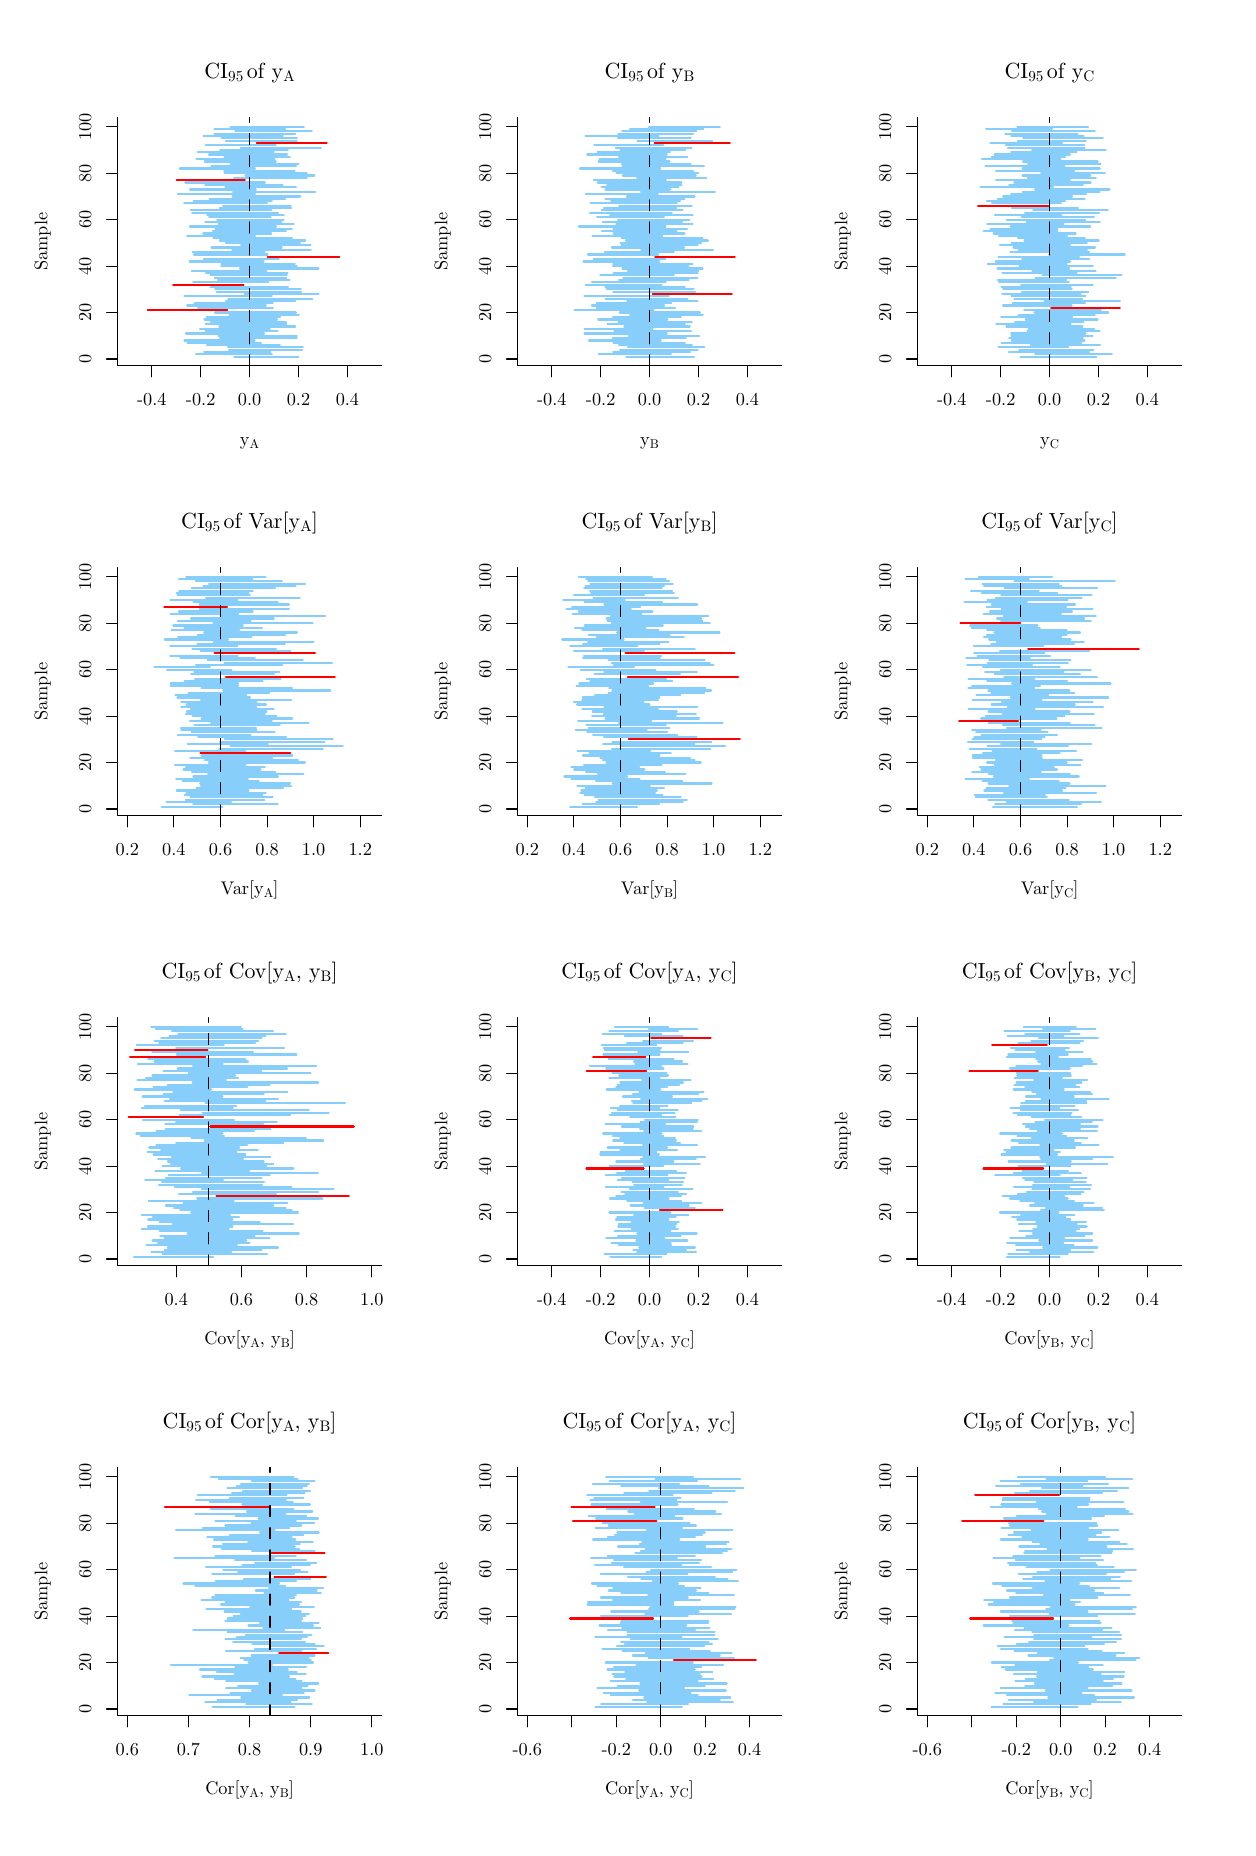
\begin{tikzpicture}[x=1pt,y=1pt]
\definecolor{fillColor}{RGB}{255,255,255}
\path[use as bounding box,fill=fillColor,fill opacity=0.00] (0,0) rectangle (433.62,650.43);
\begin{scope}
\path[clip] ( 32.47,528.21) rectangle (127.91,617.96);
\definecolor{drawColor}{RGB}{0,0,0}

\path[draw=drawColor,line width= 0.4pt,line join=round,line cap=round] (168.56,522.31) circle (  1.48);
\end{scope}
\begin{scope}
\path[clip] (  0.00,  0.00) rectangle (433.62,650.43);
\definecolor{drawColor}{RGB}{0,0,0}

\path[draw=drawColor,line width= 0.4pt,line join=round,line cap=round] ( 44.84,528.21) -- (115.54,528.21);

\path[draw=drawColor,line width= 0.4pt,line join=round,line cap=round] ( 44.84,528.21) -- ( 44.84,524.25);

\path[draw=drawColor,line width= 0.4pt,line join=round,line cap=round] ( 62.52,528.21) -- ( 62.52,524.25);

\path[draw=drawColor,line width= 0.4pt,line join=round,line cap=round] ( 80.19,528.21) -- ( 80.19,524.25);

\path[draw=drawColor,line width= 0.4pt,line join=round,line cap=round] ( 97.86,528.21) -- ( 97.86,524.25);

\path[draw=drawColor,line width= 0.4pt,line join=round,line cap=round] (115.54,528.21) -- (115.54,524.25);

\node[text=drawColor,anchor=base,inner sep=0pt, outer sep=0pt, scale=  0.66] at ( 44.84,513.96) {-0.4};

\node[text=drawColor,anchor=base,inner sep=0pt, outer sep=0pt, scale=  0.66] at ( 62.52,513.96) {-0.2};

\node[text=drawColor,anchor=base,inner sep=0pt, outer sep=0pt, scale=  0.66] at ( 80.19,513.96) {0.0};

\node[text=drawColor,anchor=base,inner sep=0pt, outer sep=0pt, scale=  0.66] at ( 97.86,513.96) {0.2};

\node[text=drawColor,anchor=base,inner sep=0pt, outer sep=0pt, scale=  0.66] at (115.54,513.96) {0.4};

\path[draw=drawColor,line width= 0.4pt,line join=round,line cap=round] ( 32.47,530.70) -- ( 32.47,614.63);

\path[draw=drawColor,line width= 0.4pt,line join=round,line cap=round] ( 32.47,530.70) -- ( 28.51,530.70);

\path[draw=drawColor,line width= 0.4pt,line join=round,line cap=round] ( 32.47,547.49) -- ( 28.51,547.49);

\path[draw=drawColor,line width= 0.4pt,line join=round,line cap=round] ( 32.47,564.27) -- ( 28.51,564.27);

\path[draw=drawColor,line width= 0.4pt,line join=round,line cap=round] ( 32.47,581.06) -- ( 28.51,581.06);

\path[draw=drawColor,line width= 0.4pt,line join=round,line cap=round] ( 32.47,597.85) -- ( 28.51,597.85);

\path[draw=drawColor,line width= 0.4pt,line join=round,line cap=round] ( 32.47,614.63) -- ( 28.51,614.63);

\node[text=drawColor,rotate= 90.00,anchor=base,inner sep=0pt, outer sep=0pt, scale=  0.66] at ( 22.97,530.70) {0};

\node[text=drawColor,rotate= 90.00,anchor=base,inner sep=0pt, outer sep=0pt, scale=  0.66] at ( 22.97,547.49) {20};

\node[text=drawColor,rotate= 90.00,anchor=base,inner sep=0pt, outer sep=0pt, scale=  0.66] at ( 22.97,564.27) {40};

\node[text=drawColor,rotate= 90.00,anchor=base,inner sep=0pt, outer sep=0pt, scale=  0.66] at ( 22.97,581.06) {60};

\node[text=drawColor,rotate= 90.00,anchor=base,inner sep=0pt, outer sep=0pt, scale=  0.66] at ( 22.97,597.85) {80};

\node[text=drawColor,rotate= 90.00,anchor=base,inner sep=0pt, outer sep=0pt, scale=  0.66] at ( 22.97,614.63) {100};

\path[draw=drawColor,line width= 0.4pt,line join=round,line cap=round] ( 32.47,617.96) --
	( 32.47,528.21) --
	(127.91,528.21);
\end{scope}
\begin{scope}
\path[clip] (  0.00,487.82) rectangle (144.54,650.43);
\definecolor{drawColor}{RGB}{0,0,0}

\node[text=drawColor,anchor=base west,inner sep=0pt, outer sep=0pt, scale=  0.79] at ( 63.86,632.21) {CI};

\node[text=drawColor,anchor=base west,inner sep=0pt, outer sep=0pt, scale=  0.55] at ( 72.44,631.02) {95};

\node[text=drawColor,anchor=base west,inner sep=0pt, outer sep=0pt, scale=  0.79] at ( 77.98,632.21) {\hspace{1.5pt}of y};

\node[text=drawColor,anchor=base west,inner sep=0pt, outer sep=0pt, scale=  0.55] at ( 92.36,631.02) {A};

\node[text=drawColor,anchor=base west,inner sep=0pt, outer sep=0pt, scale=  0.66] at ( 76.72,499.40) {y};

\node[text=drawColor,anchor=base west,inner sep=0pt, outer sep=0pt, scale=  0.46] at ( 80.20,498.41) {A};

\node[text=drawColor,rotate= 90.00,anchor=base,inner sep=0pt, outer sep=0pt, scale=  0.66] at (  7.13,573.09) {Sample};
\end{scope}
\begin{scope}
\path[clip] ( 32.47,528.21) rectangle (127.91,617.96);
\definecolor{drawColor}{RGB}{135,206,250}

\path[draw=drawColor,line width= 0.8pt,line join=round,line cap=round] ( 74.59,531.54) --
	( 97.83,531.54);

\path[draw=drawColor,line width= 0.8pt,line join=round,line cap=round] ( 60.78,532.38) --
	( 88.20,532.38);

\path[draw=drawColor,line width= 0.8pt,line join=round,line cap=round] ( 63.80,533.22) --
	( 87.75,533.22);

\path[draw=drawColor,line width= 0.8pt,line join=round,line cap=round] ( 72.70,534.06) --
	( 99.17,534.06);

\path[draw=drawColor,line width= 0.8pt,line join=round,line cap=round] ( 72.33,534.90) --
	( 99.40,534.90);

\path[draw=drawColor,line width= 0.8pt,line join=round,line cap=round] ( 64.79,535.74) --
	( 91.14,535.74);

\path[draw=drawColor,line width= 0.8pt,line join=round,line cap=round] ( 57.75,536.57) --
	( 84.32,536.57);

\path[draw=drawColor,line width= 0.8pt,line join=round,line cap=round] ( 56.64,537.41) --
	( 81.95,537.41);

\path[draw=drawColor,line width= 0.8pt,line join=round,line cap=round] ( 69.47,538.25) --
	( 97.27,538.25);

\path[draw=drawColor,line width= 0.8pt,line join=round,line cap=round] ( 68.91,539.09) --
	( 97.24,539.09);

\path[draw=drawColor,line width= 0.8pt,line join=round,line cap=round] ( 57.18,539.93) --
	( 85.44,539.93);

\path[draw=drawColor,line width= 0.8pt,line join=round,line cap=round] ( 64.22,540.77) --
	( 90.29,540.77);

\path[draw=drawColor,line width= 0.8pt,line join=round,line cap=round] ( 62.24,541.61) --
	( 87.51,541.61);

\path[draw=drawColor,line width= 0.8pt,line join=round,line cap=round] ( 69.28,542.45) --
	( 96.71,542.45);

\path[draw=drawColor,line width= 0.8pt,line join=round,line cap=round] ( 64.34,543.29) --
	( 93.49,543.29);

\path[draw=drawColor,line width= 0.8pt,line join=round,line cap=round] ( 66.10,544.13) --
	( 93.36,544.13);

\path[draw=drawColor,line width= 0.8pt,line join=round,line cap=round] ( 63.92,544.97) --
	( 90.12,544.97);

\path[draw=drawColor,line width= 0.8pt,line join=round,line cap=round] ( 64.72,545.81) --
	( 91.22,545.81);

\path[draw=drawColor,line width= 0.8pt,line join=round,line cap=round] ( 72.93,546.65) --
	( 98.01,546.65);

\path[draw=drawColor,line width= 0.8pt,line join=round,line cap=round] ( 67.67,547.49) --
	( 96.92,547.49);
\definecolor{drawColor}{RGB}{255,0,0}

\path[draw=drawColor,line width= 0.8pt,line join=round,line cap=round] ( 43.33,548.33) --
	( 72.12,548.33);
\definecolor{drawColor}{RGB}{135,206,250}

\path[draw=drawColor,line width= 0.8pt,line join=round,line cap=round] ( 61.53,549.16) --
	( 88.58,549.16);

\path[draw=drawColor,line width= 0.8pt,line join=round,line cap=round] ( 57.63,550.00) --
	( 86.04,550.00);

\path[draw=drawColor,line width= 0.8pt,line join=round,line cap=round] ( 60.27,550.84) --
	( 88.56,550.84);

\path[draw=drawColor,line width= 0.8pt,line join=round,line cap=round] ( 71.60,551.68) --
	( 96.68,551.68);

\path[draw=drawColor,line width= 0.8pt,line join=round,line cap=round] ( 72.43,552.52) --
	(102.83,552.52);

\path[draw=drawColor,line width= 0.8pt,line join=round,line cap=round] ( 56.60,553.36) --
	( 88.24,553.36);

\path[draw=drawColor,line width= 0.8pt,line join=round,line cap=round] ( 78.41,554.20) --
	(105.13,554.20);

\path[draw=drawColor,line width= 0.8pt,line join=round,line cap=round] ( 68.28,555.04) --
	( 98.78,555.04);

\path[draw=drawColor,line width= 0.8pt,line join=round,line cap=round] ( 67.72,555.88) --
	( 98.74,555.88);

\path[draw=drawColor,line width= 0.8pt,line join=round,line cap=round] ( 66.05,556.72) --
	( 94.06,556.72);
\definecolor{drawColor}{RGB}{255,0,0}

\path[draw=drawColor,line width= 0.8pt,line join=round,line cap=round] ( 52.54,557.56) --
	( 78.01,557.56);
\definecolor{drawColor}{RGB}{135,206,250}

\path[draw=drawColor,line width= 0.8pt,line join=round,line cap=round] ( 59.81,558.40) --
	( 87.00,558.40);

\path[draw=drawColor,line width= 0.8pt,line join=round,line cap=round] ( 68.72,559.24) --
	( 94.62,559.24);

\path[draw=drawColor,line width= 0.8pt,line join=round,line cap=round] ( 67.57,560.08) --
	( 93.44,560.08);

\path[draw=drawColor,line width= 0.8pt,line join=round,line cap=round] ( 66.06,560.92) --
	( 93.63,560.92);

\path[draw=drawColor,line width= 0.8pt,line join=round,line cap=round] ( 64.44,561.75) --
	( 93.94,561.75);

\path[draw=drawColor,line width= 0.8pt,line join=round,line cap=round] ( 59.23,562.59) --
	( 86.24,562.59);

\path[draw=drawColor,line width= 0.8pt,line join=round,line cap=round] ( 76.68,563.43) --
	(105.09,563.43);

\path[draw=drawColor,line width= 0.8pt,line join=round,line cap=round] ( 69.93,564.27) --
	( 97.26,564.27);

\path[draw=drawColor,line width= 0.8pt,line join=round,line cap=round] ( 69.99,565.11) --
	( 96.49,565.11);

\path[draw=drawColor,line width= 0.8pt,line join=round,line cap=round] ( 58.55,565.95) --
	( 85.18,565.95);

\path[draw=drawColor,line width= 0.8pt,line join=round,line cap=round] ( 63.63,566.79) --
	( 90.77,566.79);
\definecolor{drawColor}{RGB}{255,0,0}

\path[draw=drawColor,line width= 0.8pt,line join=round,line cap=round] ( 86.74,567.63) --
	(112.63,567.63);
\definecolor{drawColor}{RGB}{135,206,250}

\path[draw=drawColor,line width= 0.8pt,line join=round,line cap=round] ( 60.11,568.47) --
	( 86.70,568.47);

\path[draw=drawColor,line width= 0.8pt,line join=round,line cap=round] ( 59.65,569.31) --
	( 85.57,569.31);

\path[draw=drawColor,line width= 0.8pt,line join=round,line cap=round] ( 73.94,570.15) --
	(102.28,570.15);

\path[draw=drawColor,line width= 0.8pt,line join=round,line cap=round] ( 66.41,570.99) --
	( 91.83,570.99);

\path[draw=drawColor,line width= 0.8pt,line join=round,line cap=round] ( 77.10,571.83) --
	(102.25,571.83);

\path[draw=drawColor,line width= 0.8pt,line join=round,line cap=round] ( 71.62,572.67) --
	( 98.45,572.67);

\path[draw=drawColor,line width= 0.8pt,line join=round,line cap=round] ( 69.42,573.51) --
	(100.29,573.51);

\path[draw=drawColor,line width= 0.8pt,line join=round,line cap=round] ( 67.11,574.35) --
	( 95.52,574.35);

\path[draw=drawColor,line width= 0.8pt,line join=round,line cap=round] ( 57.63,575.18) --
	( 82.15,575.18);

\path[draw=drawColor,line width= 0.8pt,line join=round,line cap=round] ( 63.47,576.02) --
	( 87.98,576.02);

\path[draw=drawColor,line width= 0.8pt,line join=round,line cap=round] ( 66.94,576.86) --
	( 93.28,576.86);

\path[draw=drawColor,line width= 0.8pt,line join=round,line cap=round] ( 67.83,577.70) --
	( 95.45,577.70);

\path[draw=drawColor,line width= 0.8pt,line join=round,line cap=round] ( 58.60,578.54) --
	( 89.75,578.54);

\path[draw=drawColor,line width= 0.8pt,line join=round,line cap=round] ( 68.96,579.38) --
	( 96.13,579.38);

\path[draw=drawColor,line width= 0.8pt,line join=round,line cap=round] ( 64.11,580.22) --
	( 91.66,580.22);

\path[draw=drawColor,line width= 0.8pt,line join=round,line cap=round] ( 68.51,581.06) --
	( 92.50,581.06);

\path[draw=drawColor,line width= 0.8pt,line join=round,line cap=round] ( 65.55,581.90) --
	( 87.75,581.90);

\path[draw=drawColor,line width= 0.8pt,line join=round,line cap=round] ( 64.84,582.74) --
	( 92.57,582.74);

\path[draw=drawColor,line width= 0.8pt,line join=round,line cap=round] ( 59.46,583.58) --
	( 90.44,583.58);

\path[draw=drawColor,line width= 0.8pt,line join=round,line cap=round] ( 58.93,584.42) --
	( 88.05,584.42);

\path[draw=drawColor,line width= 0.8pt,line join=round,line cap=round] ( 69.38,585.26) --
	( 95.17,585.26);

\path[draw=drawColor,line width= 0.8pt,line join=round,line cap=round] ( 70.60,586.10) --
	( 95.06,586.10);

\path[draw=drawColor,line width= 0.8pt,line join=round,line cap=round] ( 56.56,586.94) --
	( 86.47,586.94);

\path[draw=drawColor,line width= 0.8pt,line join=round,line cap=round] ( 59.96,587.77) --
	( 88.26,587.77);

\path[draw=drawColor,line width= 0.8pt,line join=round,line cap=round] ( 65.75,588.61) --
	( 93.06,588.61);

\path[draw=drawColor,line width= 0.8pt,line join=round,line cap=round] ( 74.01,589.45) --
	( 98.46,589.45);

\path[draw=drawColor,line width= 0.8pt,line join=round,line cap=round] ( 54.24,590.29) --
	( 82.15,590.29);

\path[draw=drawColor,line width= 0.8pt,line join=round,line cap=round] ( 74.17,591.13) --
	(103.98,591.13);

\path[draw=drawColor,line width= 0.8pt,line join=round,line cap=round] ( 58.71,591.97) --
	( 82.43,591.97);

\path[draw=drawColor,line width= 0.8pt,line join=round,line cap=round] ( 71.42,592.81) --
	( 96.95,592.81);

\path[draw=drawColor,line width= 0.8pt,line join=round,line cap=round] ( 64.18,593.65) --
	( 92.13,593.65);

\path[draw=drawColor,line width= 0.8pt,line join=round,line cap=round] ( 56.95,594.49) --
	( 85.68,594.49);
\definecolor{drawColor}{RGB}{255,0,0}

\path[draw=drawColor,line width= 0.8pt,line join=round,line cap=round] ( 53.86,595.33) --
	( 78.47,595.33);
\definecolor{drawColor}{RGB}{135,206,250}

\path[draw=drawColor,line width= 0.8pt,line join=round,line cap=round] ( 74.57,596.17) --
	(100.88,596.17);

\path[draw=drawColor,line width= 0.8pt,line join=round,line cap=round] ( 78.71,597.01) --
	(103.58,597.01);

\path[draw=drawColor,line width= 0.8pt,line join=round,line cap=round] ( 71.10,597.85) --
	(100.86,597.85);

\path[draw=drawColor,line width= 0.8pt,line join=round,line cap=round] ( 71.01,598.69) --
	( 96.48,598.69);

\path[draw=drawColor,line width= 0.8pt,line join=round,line cap=round] ( 54.99,599.53) --
	( 82.14,599.53);

\path[draw=drawColor,line width= 0.8pt,line join=round,line cap=round] ( 66.42,600.37) --
	( 96.98,600.37);

\path[draw=drawColor,line width= 0.8pt,line join=round,line cap=round] ( 73.32,601.20) --
	( 97.84,601.20);

\path[draw=drawColor,line width= 0.8pt,line join=round,line cap=round] ( 64.00,602.04) --
	( 89.62,602.04);

\path[draw=drawColor,line width= 0.8pt,line join=round,line cap=round] ( 61.02,602.88) --
	( 89.22,602.88);

\path[draw=drawColor,line width= 0.8pt,line join=round,line cap=round] ( 71.08,603.72) --
	( 94.71,603.72);

\path[draw=drawColor,line width= 0.8pt,line join=round,line cap=round] ( 65.53,604.56) --
	( 93.72,604.56);

\path[draw=drawColor,line width= 0.8pt,line join=round,line cap=round] ( 61.46,605.40) --
	( 88.89,605.40);

\path[draw=drawColor,line width= 0.8pt,line join=round,line cap=round] ( 69.56,606.24) --
	( 94.03,606.24);

\path[draw=drawColor,line width= 0.8pt,line join=round,line cap=round] ( 76.97,607.08) --
	(105.90,607.08);

\path[draw=drawColor,line width= 0.8pt,line join=round,line cap=round] ( 64.29,607.92) --
	( 89.70,607.92);
\definecolor{drawColor}{RGB}{255,0,0}

\path[draw=drawColor,line width= 0.8pt,line join=round,line cap=round] ( 82.74,608.76) --
	(108.05,608.76);
\definecolor{drawColor}{RGB}{135,206,250}

\path[draw=drawColor,line width= 0.8pt,line join=round,line cap=round] ( 71.60,609.60) --
	( 97.24,609.60);

\path[draw=drawColor,line width= 0.8pt,line join=round,line cap=round] ( 70.05,610.44) --
	( 97.28,610.44);

\path[draw=drawColor,line width= 0.8pt,line join=round,line cap=round] ( 63.53,611.28) --
	( 92.18,611.28);

\path[draw=drawColor,line width= 0.8pt,line join=round,line cap=round] ( 67.40,612.12) --
	( 96.67,612.12);

\path[draw=drawColor,line width= 0.8pt,line join=round,line cap=round] ( 74.96,612.96) --
	(102.67,612.96);

\path[draw=drawColor,line width= 0.8pt,line join=round,line cap=round] ( 67.51,613.79) --
	( 93.11,613.79);

\path[draw=drawColor,line width= 0.8pt,line join=round,line cap=round] ( 73.23,614.63) --
	( 99.79,614.63);
\definecolor{drawColor}{RGB}{0,0,0}

\path[draw=drawColor,line width= 0.4pt,dash pattern=on 4pt off 4pt ,line join=round,line cap=round] ( 80.19,528.21) -- ( 80.19,617.96);
\end{scope}
\begin{scope}
\path[clip] (177.01,528.21) rectangle (272.45,617.96);
\definecolor{drawColor}{RGB}{0,0,0}

\path[draw=drawColor,line width= 0.4pt,line join=round,line cap=round] (313.10,522.31) circle (  1.48);
\end{scope}
\begin{scope}
\path[clip] (  0.00,  0.00) rectangle (433.62,650.43);
\definecolor{drawColor}{RGB}{0,0,0}

\path[draw=drawColor,line width= 0.4pt,line join=round,line cap=round] (189.38,528.21) -- (260.08,528.21);

\path[draw=drawColor,line width= 0.4pt,line join=round,line cap=round] (189.38,528.21) -- (189.38,524.25);

\path[draw=drawColor,line width= 0.4pt,line join=round,line cap=round] (207.06,528.21) -- (207.06,524.25);

\path[draw=drawColor,line width= 0.4pt,line join=round,line cap=round] (224.73,528.21) -- (224.73,524.25);

\path[draw=drawColor,line width= 0.4pt,line join=round,line cap=round] (242.40,528.21) -- (242.40,524.25);

\path[draw=drawColor,line width= 0.4pt,line join=round,line cap=round] (260.08,528.21) -- (260.08,524.25);

\node[text=drawColor,anchor=base,inner sep=0pt, outer sep=0pt, scale=  0.66] at (189.38,513.96) {-0.4};

\node[text=drawColor,anchor=base,inner sep=0pt, outer sep=0pt, scale=  0.66] at (207.06,513.96) {-0.2};

\node[text=drawColor,anchor=base,inner sep=0pt, outer sep=0pt, scale=  0.66] at (224.73,513.96) {0.0};

\node[text=drawColor,anchor=base,inner sep=0pt, outer sep=0pt, scale=  0.66] at (242.40,513.96) {0.2};

\node[text=drawColor,anchor=base,inner sep=0pt, outer sep=0pt, scale=  0.66] at (260.08,513.96) {0.4};

\path[draw=drawColor,line width= 0.4pt,line join=round,line cap=round] (177.01,530.70) -- (177.01,614.63);

\path[draw=drawColor,line width= 0.4pt,line join=round,line cap=round] (177.01,530.70) -- (173.05,530.70);

\path[draw=drawColor,line width= 0.4pt,line join=round,line cap=round] (177.01,547.49) -- (173.05,547.49);

\path[draw=drawColor,line width= 0.4pt,line join=round,line cap=round] (177.01,564.27) -- (173.05,564.27);

\path[draw=drawColor,line width= 0.4pt,line join=round,line cap=round] (177.01,581.06) -- (173.05,581.06);

\path[draw=drawColor,line width= 0.4pt,line join=round,line cap=round] (177.01,597.85) -- (173.05,597.85);

\path[draw=drawColor,line width= 0.4pt,line join=round,line cap=round] (177.01,614.63) -- (173.05,614.63);

\node[text=drawColor,rotate= 90.00,anchor=base,inner sep=0pt, outer sep=0pt, scale=  0.66] at (167.51,530.70) {0};

\node[text=drawColor,rotate= 90.00,anchor=base,inner sep=0pt, outer sep=0pt, scale=  0.66] at (167.51,547.49) {20};

\node[text=drawColor,rotate= 90.00,anchor=base,inner sep=0pt, outer sep=0pt, scale=  0.66] at (167.51,564.27) {40};

\node[text=drawColor,rotate= 90.00,anchor=base,inner sep=0pt, outer sep=0pt, scale=  0.66] at (167.51,581.06) {60};

\node[text=drawColor,rotate= 90.00,anchor=base,inner sep=0pt, outer sep=0pt, scale=  0.66] at (167.51,597.85) {80};

\node[text=drawColor,rotate= 90.00,anchor=base,inner sep=0pt, outer sep=0pt, scale=  0.66] at (167.51,614.63) {100};

\path[draw=drawColor,line width= 0.4pt,line join=round,line cap=round] (177.01,617.96) --
	(177.01,528.21) --
	(272.45,528.21);
\end{scope}
\begin{scope}
\path[clip] (144.54,487.82) rectangle (289.08,650.43);
\definecolor{drawColor}{RGB}{0,0,0}

\node[text=drawColor,anchor=base west,inner sep=0pt, outer sep=0pt, scale=  0.79] at (208.51,632.21) {CI};

\node[text=drawColor,anchor=base west,inner sep=0pt, outer sep=0pt, scale=  0.55] at (217.09,631.02) {95};

\node[text=drawColor,anchor=base west,inner sep=0pt, outer sep=0pt, scale=  0.79] at (222.63,632.21) {\hspace{1.5pt}of y};

\node[text=drawColor,anchor=base west,inner sep=0pt, outer sep=0pt, scale=  0.55] at (237.02,631.02) {B};

\node[text=drawColor,anchor=base west,inner sep=0pt, outer sep=0pt, scale=  0.66] at (221.35,499.40) {y};

\node[text=drawColor,anchor=base west,inner sep=0pt, outer sep=0pt, scale=  0.46] at (224.84,498.41) {B};

\node[text=drawColor,rotate= 90.00,anchor=base,inner sep=0pt, outer sep=0pt, scale=  0.66] at (151.67,573.09) {Sample};
\end{scope}
\begin{scope}
\path[clip] (177.01,528.21) rectangle (272.45,617.96);
\definecolor{drawColor}{RGB}{135,206,250}

\path[draw=drawColor,line width= 0.8pt,line join=round,line cap=round] (216.37,531.54) --
	(240.80,531.54);

\path[draw=drawColor,line width= 0.8pt,line join=round,line cap=round] (206.35,532.38) --
	(232.45,532.38);

\path[draw=drawColor,line width= 0.8pt,line join=round,line cap=round] (211.60,533.22) --
	(239.38,533.22);

\path[draw=drawColor,line width= 0.8pt,line join=round,line cap=round] (214.06,534.06) --
	(242.12,534.06);

\path[draw=drawColor,line width= 0.8pt,line join=round,line cap=round] (216.88,534.90) --
	(244.51,534.90);

\path[draw=drawColor,line width= 0.8pt,line join=round,line cap=round] (213.66,535.74) --
	(240.02,535.74);

\path[draw=drawColor,line width= 0.8pt,line join=round,line cap=round] (211.65,536.57) --
	(237.44,536.57);

\path[draw=drawColor,line width= 0.8pt,line join=round,line cap=round] (202.82,537.41) --
	(228.76,537.41);

\path[draw=drawColor,line width= 0.8pt,line join=round,line cap=round] (211.35,538.25) --
	(237.80,538.25);

\path[draw=drawColor,line width= 0.8pt,line join=round,line cap=round] (217.19,539.09) --
	(242.60,539.09);

\path[draw=drawColor,line width= 0.8pt,line join=round,line cap=round] (201.24,539.93) --
	(230.93,539.93);

\path[draw=drawColor,line width= 0.8pt,line join=round,line cap=round] (211.97,540.77) --
	(239.70,540.77);

\path[draw=drawColor,line width= 0.8pt,line join=round,line cap=round] (201.21,541.61) --
	(225.83,541.61);

\path[draw=drawColor,line width= 0.8pt,line join=round,line cap=round] (215.61,542.45) --
	(239.26,542.45);

\path[draw=drawColor,line width= 0.8pt,line join=round,line cap=round] (209.50,543.29) --
	(237.44,543.29);

\path[draw=drawColor,line width= 0.8pt,line join=round,line cap=round] (213.48,544.13) --
	(240.00,544.13);

\path[draw=drawColor,line width= 0.8pt,line join=round,line cap=round] (206.15,544.97) --
	(231.14,544.97);

\path[draw=drawColor,line width= 0.8pt,line join=round,line cap=round] (211.44,545.81) --
	(236.04,545.81);

\path[draw=drawColor,line width= 0.8pt,line join=round,line cap=round] (217.66,546.65) --
	(243.93,546.65);

\path[draw=drawColor,line width= 0.8pt,line join=round,line cap=round] (213.91,547.49) --
	(242.90,547.49);

\path[draw=drawColor,line width= 0.8pt,line join=round,line cap=round] (197.58,548.33) --
	(226.14,548.33);

\path[draw=drawColor,line width= 0.8pt,line join=round,line cap=round] (205.63,549.16) --
	(233.90,549.16);

\path[draw=drawColor,line width= 0.8pt,line join=round,line cap=round] (203.86,550.00) --
	(229.99,550.00);

\path[draw=drawColor,line width= 0.8pt,line join=round,line cap=round] (205.62,550.84) --
	(232.57,550.84);

\path[draw=drawColor,line width= 0.8pt,line join=round,line cap=round] (216.64,551.68) --
	(242.08,551.68);

\path[draw=drawColor,line width= 0.8pt,line join=round,line cap=round] (208.88,552.52) --
	(238.49,552.52);

\path[draw=drawColor,line width= 0.8pt,line join=round,line cap=round] (201.16,553.36) --
	(231.71,553.36);
\definecolor{drawColor}{RGB}{255,0,0}

\path[draw=drawColor,line width= 0.8pt,line join=round,line cap=round] (225.85,554.20) --
	(254.42,554.20);
\definecolor{drawColor}{RGB}{135,206,250}

\path[draw=drawColor,line width= 0.8pt,line join=round,line cap=round] (211.59,555.04) --
	(241.27,555.04);

\path[draw=drawColor,line width= 0.8pt,line join=round,line cap=round] (209.21,555.88) --
	(240.66,555.88);

\path[draw=drawColor,line width= 0.8pt,line join=round,line cap=round] (208.76,556.72) --
	(237.47,556.72);

\path[draw=drawColor,line width= 0.8pt,line join=round,line cap=round] (201.63,557.56) --
	(229.02,557.56);

\path[draw=drawColor,line width= 0.8pt,line join=round,line cap=round] (203.88,558.40) --
	(230.55,558.40);

\path[draw=drawColor,line width= 0.8pt,line join=round,line cap=round] (213.66,559.24) --
	(238.84,559.24);

\path[draw=drawColor,line width= 0.8pt,line join=round,line cap=round] (215.18,560.08) --
	(242.02,560.08);

\path[draw=drawColor,line width= 0.8pt,line join=round,line cap=round] (206.91,560.92) --
	(233.50,560.92);

\path[draw=drawColor,line width= 0.8pt,line join=round,line cap=round] (211.72,561.75) --
	(242.11,561.75);

\path[draw=drawColor,line width= 0.8pt,line join=round,line cap=round] (216.78,562.59) --
	(242.31,562.59);

\path[draw=drawColor,line width= 0.8pt,line join=round,line cap=round] (214.95,563.43) --
	(243.83,563.43);

\path[draw=drawColor,line width= 0.8pt,line join=round,line cap=round] (211.48,564.27) --
	(238.77,564.27);

\path[draw=drawColor,line width= 0.8pt,line join=round,line cap=round] (211.60,565.11) --
	(240.26,565.11);

\path[draw=drawColor,line width= 0.8pt,line join=round,line cap=round] (200.85,565.95) --
	(228.20,565.95);

\path[draw=drawColor,line width= 0.8pt,line join=round,line cap=round] (204.50,566.79) --
	(230.53,566.79);
\definecolor{drawColor}{RGB}{255,0,0}

\path[draw=drawColor,line width= 0.8pt,line join=round,line cap=round] (226.74,567.63) --
	(255.49,567.63);
\definecolor{drawColor}{RGB}{135,206,250}

\path[draw=drawColor,line width= 0.8pt,line join=round,line cap=round] (202.46,568.47) --
	(227.84,568.47);

\path[draw=drawColor,line width= 0.8pt,line join=round,line cap=round] (208.54,569.31) --
	(233.47,569.31);

\path[draw=drawColor,line width= 0.8pt,line join=round,line cap=round] (221.66,570.15) --
	(247.69,570.15);

\path[draw=drawColor,line width= 0.8pt,line join=round,line cap=round] (211.09,570.99) --
	(237.20,570.99);

\path[draw=drawColor,line width= 0.8pt,line join=round,line cap=round] (214.54,571.83) --
	(242.15,571.83);

\path[draw=drawColor,line width= 0.8pt,line join=round,line cap=round] (214.19,572.67) --
	(243.41,572.67);

\path[draw=drawColor,line width= 0.8pt,line join=round,line cap=round] (216.16,573.51) --
	(245.81,573.51);

\path[draw=drawColor,line width= 0.8pt,line join=round,line cap=round] (214.60,574.35) --
	(243.88,574.35);

\path[draw=drawColor,line width= 0.8pt,line join=round,line cap=round] (204.04,575.18) --
	(229.33,575.18);

\path[draw=drawColor,line width= 0.8pt,line join=round,line cap=round] (211.67,576.02) --
	(237.33,576.02);

\path[draw=drawColor,line width= 0.8pt,line join=round,line cap=round] (207.46,576.86) --
	(234.51,576.86);

\path[draw=drawColor,line width= 0.8pt,line join=round,line cap=round] (211.65,577.70) --
	(238.26,577.70);

\path[draw=drawColor,line width= 0.8pt,line join=round,line cap=round] (199.17,578.54) --
	(230.51,578.54);

\path[draw=drawColor,line width= 0.8pt,line join=round,line cap=round] (212.66,579.38) --
	(240.24,579.38);

\path[draw=drawColor,line width= 0.8pt,line join=round,line cap=round] (207.79,580.22) --
	(236.52,580.22);

\path[draw=drawColor,line width= 0.8pt,line join=round,line cap=round] (213.27,581.06) --
	(239.11,581.06);

\path[draw=drawColor,line width= 0.8pt,line join=round,line cap=round] (205.74,581.90) --
	(229.94,581.90);

\path[draw=drawColor,line width= 0.8pt,line join=round,line cap=round] (210.49,582.74) --
	(240.30,582.74);

\path[draw=drawColor,line width= 0.8pt,line join=round,line cap=round] (203.16,583.58) --
	(232.72,583.58);

\path[draw=drawColor,line width= 0.8pt,line join=round,line cap=round] (207.38,584.42) --
	(236.61,584.42);

\path[draw=drawColor,line width= 0.8pt,line join=round,line cap=round] (208.20,585.26) --
	(234.35,585.26);

\path[draw=drawColor,line width= 0.8pt,line join=round,line cap=round] (213.75,586.10) --
	(240.00,586.10);

\path[draw=drawColor,line width= 0.8pt,line join=round,line cap=round] (203.41,586.94) --
	(234.52,586.94);

\path[draw=drawColor,line width= 0.8pt,line join=round,line cap=round] (210.80,587.77) --
	(235.77,587.77);

\path[draw=drawColor,line width= 0.8pt,line join=round,line cap=round] (208.80,588.61) --
	(237.38,588.61);

\path[draw=drawColor,line width= 0.8pt,line join=round,line cap=round] (216.53,589.45) --
	(240.99,589.45);

\path[draw=drawColor,line width= 0.8pt,line join=round,line cap=round] (201.59,590.29) --
	(227.73,590.29);

\path[draw=drawColor,line width= 0.8pt,line join=round,line cap=round] (221.55,591.13) --
	(248.30,591.13);

\path[draw=drawColor,line width= 0.8pt,line join=round,line cap=round] (208.77,591.97) --
	(232.12,591.97);

\path[draw=drawColor,line width= 0.8pt,line join=round,line cap=round] (207.38,592.81) --
	(235.22,592.81);

\path[draw=drawColor,line width= 0.8pt,line join=round,line cap=round] (209.40,593.65) --
	(236.25,593.65);

\path[draw=drawColor,line width= 0.8pt,line join=round,line cap=round] (206.01,594.49) --
	(236.20,594.49);

\path[draw=drawColor,line width= 0.8pt,line join=round,line cap=round] (204.54,595.33) --
	(230.58,595.33);

\path[draw=drawColor,line width= 0.8pt,line join=round,line cap=round] (220.17,596.17) --
	(245.25,596.17);

\path[draw=drawColor,line width= 0.8pt,line join=round,line cap=round] (215.06,597.01) --
	(241.43,597.01);

\path[draw=drawColor,line width= 0.8pt,line join=round,line cap=round] (212.72,597.85) --
	(242.29,597.85);

\path[draw=drawColor,line width= 0.8pt,line join=round,line cap=round] (211.46,598.69) --
	(240.56,598.69);

\path[draw=drawColor,line width= 0.8pt,line join=round,line cap=round] (199.56,599.53) --
	(228.58,599.53);

\path[draw=drawColor,line width= 0.8pt,line join=round,line cap=round] (214.95,600.37) --
	(244.42,600.37);

\path[draw=drawColor,line width= 0.8pt,line join=round,line cap=round] (214.76,601.20) --
	(239.53,601.20);

\path[draw=drawColor,line width= 0.8pt,line join=round,line cap=round] (206.32,602.04) --
	(231.92,602.04);

\path[draw=drawColor,line width= 0.8pt,line join=round,line cap=round] (206.59,602.88) --
	(230.53,602.88);

\path[draw=drawColor,line width= 0.8pt,line join=round,line cap=round] (213.66,603.72) --
	(238.34,603.72);

\path[draw=drawColor,line width= 0.8pt,line join=round,line cap=round] (202.18,604.56) --
	(230.93,604.56);

\path[draw=drawColor,line width= 0.8pt,line join=round,line cap=round] (205.85,605.40) --
	(232.16,605.40);

\path[draw=drawColor,line width= 0.8pt,line join=round,line cap=round] (214.17,606.24) --
	(237.64,606.24);

\path[draw=drawColor,line width= 0.8pt,line join=round,line cap=round] (212.48,607.08) --
	(239.91,607.08);

\path[draw=drawColor,line width= 0.8pt,line join=round,line cap=round] (204.78,607.92) --
	(229.74,607.92);
\definecolor{drawColor}{RGB}{255,0,0}

\path[draw=drawColor,line width= 0.8pt,line join=round,line cap=round] (226.57,608.76) --
	(253.72,608.76);
\definecolor{drawColor}{RGB}{135,206,250}

\path[draw=drawColor,line width= 0.8pt,line join=round,line cap=round] (220.35,609.60) --
	(247.38,609.60);

\path[draw=drawColor,line width= 0.8pt,line join=round,line cap=round] (213.24,610.44) --
	(239.53,610.44);

\path[draw=drawColor,line width= 0.8pt,line join=round,line cap=round] (201.55,611.28) --
	(228.01,611.28);

\path[draw=drawColor,line width= 0.8pt,line join=round,line cap=round] (213.40,612.12) --
	(240.48,612.12);

\path[draw=drawColor,line width= 0.8pt,line join=round,line cap=round] (214.82,612.96) --
	(241.62,612.96);

\path[draw=drawColor,line width= 0.8pt,line join=round,line cap=round] (217.59,613.79) --
	(244.14,613.79);

\path[draw=drawColor,line width= 0.8pt,line join=round,line cap=round] (224.51,614.63) --
	(250.08,614.63);
\definecolor{drawColor}{RGB}{0,0,0}

\path[draw=drawColor,line width= 0.4pt,dash pattern=on 4pt off 4pt ,line join=round,line cap=round] (224.73,528.21) -- (224.73,617.96);
\end{scope}
\begin{scope}
\path[clip] (321.55,528.21) rectangle (416.99,617.96);
\definecolor{drawColor}{RGB}{0,0,0}

\path[draw=drawColor,line width= 0.4pt,line join=round,line cap=round] (457.64,522.31) circle (  1.48);
\end{scope}
\begin{scope}
\path[clip] (  0.00,  0.00) rectangle (433.62,650.43);
\definecolor{drawColor}{RGB}{0,0,0}

\path[draw=drawColor,line width= 0.4pt,line join=round,line cap=round] (333.92,528.21) -- (404.62,528.21);

\path[draw=drawColor,line width= 0.4pt,line join=round,line cap=round] (333.92,528.21) -- (333.92,524.25);

\path[draw=drawColor,line width= 0.4pt,line join=round,line cap=round] (351.60,528.21) -- (351.60,524.25);

\path[draw=drawColor,line width= 0.4pt,line join=round,line cap=round] (369.27,528.21) -- (369.27,524.25);

\path[draw=drawColor,line width= 0.4pt,line join=round,line cap=round] (386.94,528.21) -- (386.94,524.25);

\path[draw=drawColor,line width= 0.4pt,line join=round,line cap=round] (404.62,528.21) -- (404.62,524.25);

\node[text=drawColor,anchor=base,inner sep=0pt, outer sep=0pt, scale=  0.66] at (333.92,513.96) {-0.4};

\node[text=drawColor,anchor=base,inner sep=0pt, outer sep=0pt, scale=  0.66] at (351.60,513.96) {-0.2};

\node[text=drawColor,anchor=base,inner sep=0pt, outer sep=0pt, scale=  0.66] at (369.27,513.96) {0.0};

\node[text=drawColor,anchor=base,inner sep=0pt, outer sep=0pt, scale=  0.66] at (386.94,513.96) {0.2};

\node[text=drawColor,anchor=base,inner sep=0pt, outer sep=0pt, scale=  0.66] at (404.62,513.96) {0.4};

\path[draw=drawColor,line width= 0.4pt,line join=round,line cap=round] (321.55,530.70) -- (321.55,614.63);

\path[draw=drawColor,line width= 0.4pt,line join=round,line cap=round] (321.55,530.70) -- (317.59,530.70);

\path[draw=drawColor,line width= 0.4pt,line join=round,line cap=round] (321.55,547.49) -- (317.59,547.49);

\path[draw=drawColor,line width= 0.4pt,line join=round,line cap=round] (321.55,564.27) -- (317.59,564.27);

\path[draw=drawColor,line width= 0.4pt,line join=round,line cap=round] (321.55,581.06) -- (317.59,581.06);

\path[draw=drawColor,line width= 0.4pt,line join=round,line cap=round] (321.55,597.85) -- (317.59,597.85);

\path[draw=drawColor,line width= 0.4pt,line join=round,line cap=round] (321.55,614.63) -- (317.59,614.63);

\node[text=drawColor,rotate= 90.00,anchor=base,inner sep=0pt, outer sep=0pt, scale=  0.66] at (312.05,530.70) {0};

\node[text=drawColor,rotate= 90.00,anchor=base,inner sep=0pt, outer sep=0pt, scale=  0.66] at (312.05,547.49) {20};

\node[text=drawColor,rotate= 90.00,anchor=base,inner sep=0pt, outer sep=0pt, scale=  0.66] at (312.05,564.27) {40};

\node[text=drawColor,rotate= 90.00,anchor=base,inner sep=0pt, outer sep=0pt, scale=  0.66] at (312.05,581.06) {60};

\node[text=drawColor,rotate= 90.00,anchor=base,inner sep=0pt, outer sep=0pt, scale=  0.66] at (312.05,597.85) {80};

\node[text=drawColor,rotate= 90.00,anchor=base,inner sep=0pt, outer sep=0pt, scale=  0.66] at (312.05,614.63) {100};

\path[draw=drawColor,line width= 0.4pt,line join=round,line cap=round] (321.55,617.96) --
	(321.55,528.21) --
	(416.99,528.21);
\end{scope}
\begin{scope}
\path[clip] (289.08,487.82) rectangle (433.62,650.43);
\definecolor{drawColor}{RGB}{0,0,0}

\node[text=drawColor,anchor=base west,inner sep=0pt, outer sep=0pt, scale=  0.79] at (353.02,632.21) {CI};

\node[text=drawColor,anchor=base west,inner sep=0pt, outer sep=0pt, scale=  0.55] at (361.59,631.02) {95};

\node[text=drawColor,anchor=base west,inner sep=0pt, outer sep=0pt, scale=  0.79] at (367.14,632.21) {\hspace{1.5pt}of y};

\node[text=drawColor,anchor=base west,inner sep=0pt, outer sep=0pt, scale=  0.55] at (381.52,631.02) {C};

\node[text=drawColor,anchor=base west,inner sep=0pt, outer sep=0pt, scale=  0.66] at (365.86,499.40) {y};

\node[text=drawColor,anchor=base west,inner sep=0pt, outer sep=0pt, scale=  0.46] at (369.34,498.41) {C};

\node[text=drawColor,rotate= 90.00,anchor=base,inner sep=0pt, outer sep=0pt, scale=  0.66] at (296.21,573.09) {Sample};
\end{scope}
\begin{scope}
\path[clip] (321.55,528.21) rectangle (416.99,617.96);
\definecolor{drawColor}{RGB}{135,206,250}

\path[draw=drawColor,line width= 0.8pt,line join=round,line cap=round] (358.74,531.54) --
	(386.11,531.54);

\path[draw=drawColor,line width= 0.8pt,line join=round,line cap=round] (364.06,532.38) --
	(391.72,532.38);

\path[draw=drawColor,line width= 0.8pt,line join=round,line cap=round] (354.57,533.22) --
	(383.56,533.22);

\path[draw=drawColor,line width= 0.8pt,line join=round,line cap=round] (358.29,534.06) --
	(385.08,534.06);

\path[draw=drawColor,line width= 0.8pt,line join=round,line cap=round] (350.83,534.90) --
	(376.02,534.90);

\path[draw=drawColor,line width= 0.8pt,line join=round,line cap=round] (362.45,535.74) --
	(387.50,535.74);

\path[draw=drawColor,line width= 0.8pt,line join=round,line cap=round] (351.96,536.57) --
	(380.64,536.57);

\path[draw=drawColor,line width= 0.8pt,line join=round,line cap=round] (355.55,537.41) --
	(381.86,537.41);

\path[draw=drawColor,line width= 0.8pt,line join=round,line cap=round] (354.67,538.25) --
	(381.23,538.25);

\path[draw=drawColor,line width= 0.8pt,line join=round,line cap=round] (355.50,539.09) --
	(384.79,539.09);

\path[draw=drawColor,line width= 0.8pt,line join=round,line cap=round] (355.39,539.93) --
	(382.23,539.93);

\path[draw=drawColor,line width= 0.8pt,line join=round,line cap=round] (361.25,540.77) --
	(387.33,540.77);

\path[draw=drawColor,line width= 0.8pt,line join=round,line cap=round] (361.61,541.61) --
	(385.40,541.61);

\path[draw=drawColor,line width= 0.8pt,line join=round,line cap=round] (353.66,542.45) --
	(381.15,542.45);

\path[draw=drawColor,line width= 0.8pt,line join=round,line cap=round] (350.01,543.29) --
	(376.88,543.29);

\path[draw=drawColor,line width= 0.8pt,line join=round,line cap=round] (356.77,544.13) --
	(381.49,544.13);

\path[draw=drawColor,line width= 0.8pt,line join=round,line cap=round] (360.64,544.97) --
	(386.58,544.97);

\path[draw=drawColor,line width= 0.8pt,line join=round,line cap=round] (351.75,545.81) --
	(377.45,545.81);

\path[draw=drawColor,line width= 0.8pt,line join=round,line cap=round] (358.02,546.65) --
	(385.62,546.65);

\path[draw=drawColor,line width= 0.8pt,line join=round,line cap=round] (363.81,547.49) --
	(390.45,547.49);

\path[draw=drawColor,line width= 0.8pt,line join=round,line cap=round] (360.08,548.33) --
	(387.81,548.33);
\definecolor{drawColor}{RGB}{255,0,0}

\path[draw=drawColor,line width= 0.8pt,line join=round,line cap=round] (369.86,549.16) --
	(394.67,549.16);
\definecolor{drawColor}{RGB}{135,206,250}

\path[draw=drawColor,line width= 0.8pt,line join=round,line cap=round] (352.45,550.00) --
	(377.22,550.00);

\path[draw=drawColor,line width= 0.8pt,line join=round,line cap=round] (355.93,550.84) --
	(382.07,550.84);

\path[draw=drawColor,line width= 0.8pt,line join=round,line cap=round] (367.38,551.68) --
	(394.69,551.68);

\path[draw=drawColor,line width= 0.8pt,line join=round,line cap=round] (356.57,552.52) --
	(380.97,552.52);

\path[draw=drawColor,line width= 0.8pt,line join=round,line cap=round] (355.49,553.36) --
	(382.22,553.36);

\path[draw=drawColor,line width= 0.8pt,line join=round,line cap=round] (352.12,554.20) --
	(380.47,554.20);

\path[draw=drawColor,line width= 0.8pt,line join=round,line cap=round] (359.15,555.04) --
	(383.29,555.04);

\path[draw=drawColor,line width= 0.8pt,line join=round,line cap=round] (352.50,555.88) --
	(377.27,555.88);

\path[draw=drawColor,line width= 0.8pt,line join=round,line cap=round] (351.89,556.72) --
	(376.90,556.72);

\path[draw=drawColor,line width= 0.8pt,line join=round,line cap=round] (358.96,557.56) --
	(384.91,557.56);

\path[draw=drawColor,line width= 0.8pt,line join=round,line cap=round] (350.92,558.40) --
	(376.16,558.40);

\path[draw=drawColor,line width= 0.8pt,line join=round,line cap=round] (350.55,559.24) --
	(375.27,559.24);

\path[draw=drawColor,line width= 0.8pt,line join=round,line cap=round] (364.18,560.08) --
	(393.22,560.08);

\path[draw=drawColor,line width= 0.8pt,line join=round,line cap=round] (366.66,560.92) --
	(395.23,560.92);

\path[draw=drawColor,line width= 0.8pt,line join=round,line cap=round] (352.21,561.75) --
	(379.07,561.75);

\path[draw=drawColor,line width= 0.8pt,line join=round,line cap=round] (363.02,562.59) --
	(385.92,562.59);

\path[draw=drawColor,line width= 0.8pt,line join=round,line cap=round] (350.44,563.43) --
	(376.34,563.43);

\path[draw=drawColor,line width= 0.8pt,line join=round,line cap=round] (358.38,564.27) --
	(384.87,564.27);

\path[draw=drawColor,line width= 0.8pt,line join=round,line cap=round] (346.91,565.11) --
	(375.43,565.11);

\path[draw=drawColor,line width= 0.8pt,line join=round,line cap=round] (349.78,565.95) --
	(376.63,565.95);

\path[draw=drawColor,line width= 0.8pt,line join=round,line cap=round] (359.39,566.79) --
	(383.64,566.79);

\path[draw=drawColor,line width= 0.8pt,line join=round,line cap=round] (350.76,567.63) --
	(379.89,567.63);

\path[draw=drawColor,line width= 0.8pt,line join=round,line cap=round] (369.19,568.47) --
	(396.40,568.47);

\path[draw=drawColor,line width= 0.8pt,line join=round,line cap=round] (355.12,569.31) --
	(383.56,569.31);

\path[draw=drawColor,line width= 0.8pt,line join=round,line cap=round] (358.02,570.15) --
	(382.80,570.15);

\path[draw=drawColor,line width= 0.8pt,line join=round,line cap=round] (356.20,570.99) --
	(385.67,570.99);

\path[draw=drawColor,line width= 0.8pt,line join=round,line cap=round] (351.34,571.83) --
	(376.62,571.83);

\path[draw=drawColor,line width= 0.8pt,line join=round,line cap=round] (355.54,572.67) --
	(382.73,572.67);

\path[draw=drawColor,line width= 0.8pt,line join=round,line cap=round] (360.19,573.51) --
	(387.02,573.51);

\path[draw=drawColor,line width= 0.8pt,line join=round,line cap=round] (357.78,574.35) --
	(382.00,574.35);

\path[draw=drawColor,line width= 0.8pt,line join=round,line cap=round] (350.96,575.18) --
	(375.63,575.18);

\path[draw=drawColor,line width= 0.8pt,line join=round,line cap=round] (349.05,576.02) --
	(378.67,576.02);

\path[draw=drawColor,line width= 0.8pt,line join=round,line cap=round] (345.40,576.86) --
	(372.07,576.86);

\path[draw=drawColor,line width= 0.8pt,line join=round,line cap=round] (347.90,577.70) --
	(372.12,577.70);

\path[draw=drawColor,line width= 0.8pt,line join=round,line cap=round] (355.20,578.54) --
	(383.93,578.54);

\path[draw=drawColor,line width= 0.8pt,line join=round,line cap=round] (346.70,579.38) --
	(374.29,579.38);

\path[draw=drawColor,line width= 0.8pt,line join=round,line cap=round] (360.99,580.22) --
	(387.41,580.22);

\path[draw=drawColor,line width= 0.8pt,line join=round,line cap=round] (353.82,581.06) --
	(382.14,581.06);

\path[draw=drawColor,line width= 0.8pt,line join=round,line cap=round] (359.18,581.90) --
	(385.30,581.90);

\path[draw=drawColor,line width= 0.8pt,line join=round,line cap=round] (349.51,582.74) --
	(373.55,582.74);

\path[draw=drawColor,line width= 0.8pt,line join=round,line cap=round] (360.39,583.58) --
	(387.11,583.58);

\path[draw=drawColor,line width= 0.8pt,line join=round,line cap=round] (363.34,584.42) --
	(390.27,584.42);

\path[draw=drawColor,line width= 0.8pt,line join=round,line cap=round] (355.68,585.26) --
	(379.56,585.26);
\definecolor{drawColor}{RGB}{255,0,0}

\path[draw=drawColor,line width= 0.8pt,line join=round,line cap=round] (343.41,586.10) --
	(368.84,586.10);
\definecolor{drawColor}{RGB}{135,206,250}

\path[draw=drawColor,line width= 0.8pt,line join=round,line cap=round] (348.47,586.94) --
	(373.45,586.94);

\path[draw=drawColor,line width= 0.8pt,line join=round,line cap=round] (346.63,587.77) --
	(374.84,587.77);

\path[draw=drawColor,line width= 0.8pt,line join=round,line cap=round] (350.51,588.61) --
	(381.90,588.61);

\path[draw=drawColor,line width= 0.8pt,line join=round,line cap=round] (352.49,589.45) --
	(377.40,589.45);

\path[draw=drawColor,line width= 0.8pt,line join=round,line cap=round] (355.33,590.29) --
	(382.49,590.29);

\path[draw=drawColor,line width= 0.8pt,line join=round,line cap=round] (359.52,591.13) --
	(387.36,591.13);

\path[draw=drawColor,line width= 0.8pt,line join=round,line cap=round] (363.97,591.97) --
	(390.90,591.97);

\path[draw=drawColor,line width= 0.8pt,line join=round,line cap=round] (344.30,592.81) --
	(370.55,592.81);

\path[draw=drawColor,line width= 0.8pt,line join=round,line cap=round] (354.67,593.65) --
	(381.32,593.65);

\path[draw=drawColor,line width= 0.8pt,line join=round,line cap=round] (356.52,594.49) --
	(384.09,594.49);

\path[draw=drawColor,line width= 0.8pt,line join=round,line cap=round] (349.93,595.33) --
	(376.58,595.33);

\path[draw=drawColor,line width= 0.8pt,line join=round,line cap=round] (361.33,596.17) --
	(385.98,596.17);

\path[draw=drawColor,line width= 0.8pt,line join=round,line cap=round] (359.48,597.01) --
	(383.94,597.01);

\path[draw=drawColor,line width= 0.8pt,line join=round,line cap=round] (366.18,597.85) --
	(389.27,597.85);

\path[draw=drawColor,line width= 0.8pt,line join=round,line cap=round] (349.89,598.69) --
	(378.21,598.69);

\path[draw=drawColor,line width= 0.8pt,line join=round,line cap=round] (359.50,599.53) --
	(387.37,599.53);

\path[draw=drawColor,line width= 0.8pt,line join=round,line cap=round] (346.06,600.37) --
	(374.72,600.37);

\path[draw=drawColor,line width= 0.8pt,line join=round,line cap=round] (361.46,601.20) --
	(387.69,601.20);

\path[draw=drawColor,line width= 0.8pt,line join=round,line cap=round] (359.63,602.04) --
	(386.65,602.04);

\path[draw=drawColor,line width= 0.8pt,line join=round,line cap=round] (344.78,602.88) --
	(373.22,602.88);

\path[draw=drawColor,line width= 0.8pt,line join=round,line cap=round] (348.28,603.72) --
	(374.89,603.72);

\path[draw=drawColor,line width= 0.8pt,line join=round,line cap=round] (349.39,604.56) --
	(376.61,604.56);

\path[draw=drawColor,line width= 0.8pt,line join=round,line cap=round] (355.35,605.40) --
	(378.99,605.40);

\path[draw=drawColor,line width= 0.8pt,line join=round,line cap=round] (362.89,606.24) --
	(389.59,606.24);

\path[draw=drawColor,line width= 0.8pt,line join=round,line cap=round] (354.18,607.08) --
	(381.89,607.08);

\path[draw=drawColor,line width= 0.8pt,line join=round,line cap=round] (353.44,607.92) --
	(381.82,607.92);

\path[draw=drawColor,line width= 0.8pt,line join=round,line cap=round] (347.85,608.76) --
	(373.82,608.76);

\path[draw=drawColor,line width= 0.8pt,line join=round,line cap=round] (357.75,609.60) --
	(382.30,609.60);

\path[draw=drawColor,line width= 0.8pt,line join=round,line cap=round] (359.73,610.44) --
	(388.48,610.44);

\path[draw=drawColor,line width= 0.8pt,line join=round,line cap=round] (355.40,611.28) --
	(381.66,611.28);

\path[draw=drawColor,line width= 0.8pt,line join=round,line cap=round] (353.32,612.12) --
	(379.39,612.12);

\path[draw=drawColor,line width= 0.8pt,line join=round,line cap=round] (355.69,612.96) --
	(385.59,612.96);

\path[draw=drawColor,line width= 0.8pt,line join=round,line cap=round] (346.36,613.79) --
	(370.14,613.79);

\path[draw=drawColor,line width= 0.8pt,line join=round,line cap=round] (357.62,614.63) --
	(383.20,614.63);
\definecolor{drawColor}{RGB}{0,0,0}

\path[draw=drawColor,line width= 0.4pt,dash pattern=on 4pt off 4pt ,line join=round,line cap=round] (369.27,528.21) -- (369.27,617.96);
\end{scope}
\begin{scope}
\path[clip] ( 32.47,365.61) rectangle (127.91,455.35);
\definecolor{drawColor}{RGB}{0,0,0}

\path[draw=drawColor,line width= 0.4pt,line join=round,line cap=round] (103.33,359.70) circle (  1.48);
\end{scope}
\begin{scope}
\path[clip] (  0.00,  0.00) rectangle (433.62,650.43);
\definecolor{drawColor}{RGB}{0,0,0}

\path[draw=drawColor,line width= 0.4pt,line join=round,line cap=round] ( 36.01,365.61) -- (120.17,365.61);

\path[draw=drawColor,line width= 0.4pt,line join=round,line cap=round] ( 36.01,365.61) -- ( 36.01,361.65);

\path[draw=drawColor,line width= 0.4pt,line join=round,line cap=round] ( 52.84,365.61) -- ( 52.84,361.65);

\path[draw=drawColor,line width= 0.4pt,line join=round,line cap=round] ( 69.67,365.61) -- ( 69.67,361.65);

\path[draw=drawColor,line width= 0.4pt,line join=round,line cap=round] ( 86.50,365.61) -- ( 86.50,361.65);

\path[draw=drawColor,line width= 0.4pt,line join=round,line cap=round] (103.33,365.61) -- (103.33,361.65);

\path[draw=drawColor,line width= 0.4pt,line join=round,line cap=round] (120.17,365.61) -- (120.17,361.65);

\node[text=drawColor,anchor=base,inner sep=0pt, outer sep=0pt, scale=  0.66] at ( 36.01,351.35) {0.2};

\node[text=drawColor,anchor=base,inner sep=0pt, outer sep=0pt, scale=  0.66] at ( 52.84,351.35) {0.4};

\node[text=drawColor,anchor=base,inner sep=0pt, outer sep=0pt, scale=  0.66] at ( 69.67,351.35) {0.6};

\node[text=drawColor,anchor=base,inner sep=0pt, outer sep=0pt, scale=  0.66] at ( 86.50,351.35) {0.8};

\node[text=drawColor,anchor=base,inner sep=0pt, outer sep=0pt, scale=  0.66] at (103.33,351.35) {1.0};

\node[text=drawColor,anchor=base,inner sep=0pt, outer sep=0pt, scale=  0.66] at (120.17,351.35) {1.2};

\path[draw=drawColor,line width= 0.4pt,line join=round,line cap=round] ( 32.47,368.09) -- ( 32.47,452.03);

\path[draw=drawColor,line width= 0.4pt,line join=round,line cap=round] ( 32.47,368.09) -- ( 28.51,368.09);

\path[draw=drawColor,line width= 0.4pt,line join=round,line cap=round] ( 32.47,384.88) -- ( 28.51,384.88);

\path[draw=drawColor,line width= 0.4pt,line join=round,line cap=round] ( 32.47,401.67) -- ( 28.51,401.67);

\path[draw=drawColor,line width= 0.4pt,line join=round,line cap=round] ( 32.47,418.45) -- ( 28.51,418.45);

\path[draw=drawColor,line width= 0.4pt,line join=round,line cap=round] ( 32.47,435.24) -- ( 28.51,435.24);

\path[draw=drawColor,line width= 0.4pt,line join=round,line cap=round] ( 32.47,452.03) -- ( 28.51,452.03);

\node[text=drawColor,rotate= 90.00,anchor=base,inner sep=0pt, outer sep=0pt, scale=  0.66] at ( 22.97,368.09) {0};

\node[text=drawColor,rotate= 90.00,anchor=base,inner sep=0pt, outer sep=0pt, scale=  0.66] at ( 22.97,384.88) {20};

\node[text=drawColor,rotate= 90.00,anchor=base,inner sep=0pt, outer sep=0pt, scale=  0.66] at ( 22.97,401.67) {40};

\node[text=drawColor,rotate= 90.00,anchor=base,inner sep=0pt, outer sep=0pt, scale=  0.66] at ( 22.97,418.45) {60};

\node[text=drawColor,rotate= 90.00,anchor=base,inner sep=0pt, outer sep=0pt, scale=  0.66] at ( 22.97,435.24) {80};

\node[text=drawColor,rotate= 90.00,anchor=base,inner sep=0pt, outer sep=0pt, scale=  0.66] at ( 22.97,452.03) {100};

\path[draw=drawColor,line width= 0.4pt,line join=round,line cap=round] ( 32.47,455.35) --
	( 32.47,365.61) --
	(127.91,365.61);
\end{scope}
\begin{scope}
\path[clip] (  0.00,325.21) rectangle (144.54,487.82);
\definecolor{drawColor}{RGB}{0,0,0}

\node[text=drawColor,anchor=base west,inner sep=0pt, outer sep=0pt, scale=  0.79] at ( 55.49,469.61) {CI};

\node[text=drawColor,anchor=base west,inner sep=0pt, outer sep=0pt, scale=  0.55] at ( 64.07,468.41) {95};

\node[text=drawColor,anchor=base west,inner sep=0pt, outer sep=0pt, scale=  0.79] at ( 69.61,469.61) {\hspace{1.5pt}of Var[y};

\node[text=drawColor,anchor=base west,inner sep=0pt, outer sep=0pt, scale=  0.55] at ( 98.53,468.41) {A};

\node[text=drawColor,anchor=base west,inner sep=0pt, outer sep=0pt, scale=  0.79] at (102.69,469.61) {]};

\node[text=drawColor,anchor=base west,inner sep=0pt, outer sep=0pt, scale=  0.66] at ( 69.74,337.16) {Var[y};

\node[text=drawColor,anchor=base west,inner sep=0pt, outer sep=0pt, scale=  0.46] at ( 85.34,336.17) {A};

\node[text=drawColor,anchor=base west,inner sep=0pt, outer sep=0pt, scale=  0.66] at ( 88.80,337.16) {]};

\node[text=drawColor,rotate= 90.00,anchor=base,inner sep=0pt, outer sep=0pt, scale=  0.66] at (  7.13,410.48) {Sample};
\end{scope}
\begin{scope}
\path[clip] ( 32.47,365.61) rectangle (127.91,455.35);
\definecolor{drawColor}{RGB}{135,206,250}

\path[draw=drawColor,line width= 0.8pt,line join=round,line cap=round] ( 70.33,368.93) --
	( 48.40,368.93);

\path[draw=drawColor,line width= 0.8pt,line join=round,line cap=round] ( 90.34,369.77) --
	( 59.83,369.77);

\path[draw=drawColor,line width= 0.8pt,line join=round,line cap=round] ( 73.47,370.61) --
	( 50.19,370.61);

\path[draw=drawColor,line width= 0.8pt,line join=round,line cap=round] ( 85.53,371.45) --
	( 57.08,371.45);

\path[draw=drawColor,line width= 0.8pt,line join=round,line cap=round] ( 88.51,372.29) --
	( 58.78,372.29);

\path[draw=drawColor,line width= 0.8pt,line join=round,line cap=round] ( 84.86,373.13) --
	( 56.70,373.13);

\path[draw=drawColor,line width= 0.8pt,line join=round,line cap=round] ( 85.96,373.97) --
	( 57.33,373.97);

\path[draw=drawColor,line width= 0.8pt,line join=round,line cap=round] ( 79.82,374.81) --
	( 53.82,374.81);

\path[draw=drawColor,line width= 0.8pt,line join=round,line cap=round] ( 92.34,375.65) --
	( 60.97,375.65);

\path[draw=drawColor,line width= 0.8pt,line join=round,line cap=round] ( 95.15,376.48) --
	( 62.58,376.48);

\path[draw=drawColor,line width= 0.8pt,line join=round,line cap=round] ( 94.75,377.32) --
	( 62.34,377.32);

\path[draw=drawColor,line width= 0.8pt,line join=round,line cap=round] ( 83.51,378.16) --
	( 55.93,378.16);

\path[draw=drawColor,line width= 0.8pt,line join=round,line cap=round] ( 79.58,379.00) --
	( 53.68,379.00);

\path[draw=drawColor,line width= 0.8pt,line join=round,line cap=round] ( 90.42,379.84) --
	( 59.87,379.84);

\path[draw=drawColor,line width= 0.8pt,line join=round,line cap=round] ( 99.64,380.68) --
	( 65.14,380.68);

\path[draw=drawColor,line width= 0.8pt,line join=round,line cap=round] ( 89.49,381.52) --
	( 59.34,381.52);

\path[draw=drawColor,line width= 0.8pt,line join=round,line cap=round] ( 84.13,382.36) --
	( 56.28,382.36);

\path[draw=drawColor,line width= 0.8pt,line join=round,line cap=round] ( 85.65,383.20) --
	( 57.15,383.20);

\path[draw=drawColor,line width= 0.8pt,line join=round,line cap=round] ( 78.73,384.04) --
	( 53.20,384.04);

\path[draw=drawColor,line width= 0.8pt,line join=round,line cap=round] (100.17,384.88) --
	( 65.44,384.88);

\path[draw=drawColor,line width= 0.8pt,line join=round,line cap=round] ( 97.66,385.72) --
	( 64.01,385.72);

\path[draw=drawColor,line width= 0.8pt,line join=round,line cap=round] ( 88.41,386.56) --
	( 58.73,386.56);

\path[draw=drawColor,line width= 0.8pt,line join=round,line cap=round] ( 95.59,387.40) --
	( 62.83,387.40);
\definecolor{drawColor}{RGB}{255,0,0}

\path[draw=drawColor,line width= 0.8pt,line join=round,line cap=round] ( 94.89,388.24) --
	( 62.43,388.24);
\definecolor{drawColor}{RGB}{135,206,250}

\path[draw=drawColor,line width= 0.8pt,line join=round,line cap=round] ( 78.69,389.08) --
	( 53.18,389.08);

\path[draw=drawColor,line width= 0.8pt,line join=round,line cap=round] (106.64,389.91) --
	( 69.14,389.91);

\path[draw=drawColor,line width= 0.8pt,line join=round,line cap=round] (113.91,390.75) --
	( 73.29,390.75);

\path[draw=drawColor,line width= 0.8pt,line join=round,line cap=round] ( 86.76,391.59) --
	( 57.78,391.59);

\path[draw=drawColor,line width= 0.8pt,line join=round,line cap=round] (107.23,392.43) --
	( 69.47,392.43);

\path[draw=drawColor,line width= 0.8pt,line join=round,line cap=round] (110.28,393.27) --
	( 71.22,393.27);

\path[draw=drawColor,line width= 0.8pt,line join=round,line cap=round] ( 93.41,394.11) --
	( 61.58,394.11);

\path[draw=drawColor,line width= 0.8pt,line join=round,line cap=round] ( 80.57,394.95) --
	( 54.25,394.95);

\path[draw=drawColor,line width= 0.8pt,line join=round,line cap=round] ( 89.19,395.79) --
	( 59.17,395.79);

\path[draw=drawColor,line width= 0.8pt,line join=round,line cap=round] ( 82.68,396.63) --
	( 55.45,396.63);

\path[draw=drawColor,line width= 0.8pt,line join=round,line cap=round] ( 82.53,397.47) --
	( 55.36,397.47);

\path[draw=drawColor,line width= 0.8pt,line join=round,line cap=round] ( 91.12,398.31) --
	( 60.27,398.31);

\path[draw=drawColor,line width= 0.8pt,line join=round,line cap=round] (101.54,399.15) --
	( 66.23,399.15);

\path[draw=drawColor,line width= 0.8pt,line join=round,line cap=round] ( 88.22,399.99) --
	( 58.62,399.99);

\path[draw=drawColor,line width= 0.8pt,line join=round,line cap=round] ( 95.58,400.83) --
	( 62.82,400.83);

\path[draw=drawColor,line width= 0.8pt,line join=round,line cap=round] ( 89.89,401.67) --
	( 59.57,401.67);

\path[draw=drawColor,line width= 0.8pt,line join=round,line cap=round] ( 85.65,402.50) --
	( 57.15,402.50);

\path[draw=drawColor,line width= 0.8pt,line join=round,line cap=round] ( 86.31,403.34) --
	( 57.52,403.34);

\path[draw=drawColor,line width= 0.8pt,line join=round,line cap=round] ( 88.90,404.18) --
	( 59.00,404.18);

\path[draw=drawColor,line width= 0.8pt,line join=round,line cap=round] ( 82.66,405.02) --
	( 55.44,405.02);

\path[draw=drawColor,line width= 0.8pt,line join=round,line cap=round] ( 86.08,405.86) --
	( 57.39,405.86);

\path[draw=drawColor,line width= 0.8pt,line join=round,line cap=round] ( 82.76,406.70) --
	( 55.50,406.70);

\path[draw=drawColor,line width= 0.8pt,line join=round,line cap=round] ( 95.19,407.54) --
	( 62.60,407.54);

\path[draw=drawColor,line width= 0.8pt,line join=round,line cap=round] ( 80.33,408.38) --
	( 54.11,408.38);

\path[draw=drawColor,line width= 0.8pt,line join=round,line cap=round] ( 79.05,409.22) --
	( 53.38,409.22);

\path[draw=drawColor,line width= 0.8pt,line join=round,line cap=round] ( 87.33,410.06) --
	( 58.11,410.06);

\path[draw=drawColor,line width= 0.8pt,line join=round,line cap=round] (109.35,410.90) --
	( 70.69,410.90);

\path[draw=drawColor,line width= 0.8pt,line join=round,line cap=round] ( 95.56,411.74) --
	( 62.81,411.74);

\path[draw=drawColor,line width= 0.8pt,line join=round,line cap=round] ( 76.05,412.58) --
	( 51.67,412.58);

\path[draw=drawColor,line width= 0.8pt,line join=round,line cap=round] ( 76.05,413.42) --
	( 51.67,413.42);

\path[draw=drawColor,line width= 0.8pt,line join=round,line cap=round] ( 84.85,414.26) --
	( 56.69,414.26);

\path[draw=drawColor,line width= 0.8pt,line join=round,line cap=round] ( 91.36,415.10) --
	( 60.41,415.10);
\definecolor{drawColor}{RGB}{255,0,0}

\path[draw=drawColor,line width= 0.8pt,line join=round,line cap=round] (110.98,415.93) --
	( 71.62,415.93);
\definecolor{drawColor}{RGB}{135,206,250}

\path[draw=drawColor,line width= 0.8pt,line join=round,line cap=round] ( 89.06,416.77) --
	( 59.10,416.77);

\path[draw=drawColor,line width= 0.8pt,line join=round,line cap=round] ( 91.01,417.61) --
	( 60.21,417.61);

\path[draw=drawColor,line width= 0.8pt,line join=round,line cap=round] ( 73.67,418.45) --
	( 50.30,418.45);

\path[draw=drawColor,line width= 0.8pt,line join=round,line cap=round] ( 65.83,419.29) --
	( 45.83,419.29);

\path[draw=drawColor,line width= 0.8pt,line join=round,line cap=round] ( 92.00,420.13) --
	( 60.78,420.13);

\path[draw=drawColor,line width= 0.8pt,line join=round,line cap=round] (110.03,420.97) --
	( 71.07,420.97);

\path[draw=drawColor,line width= 0.8pt,line join=round,line cap=round] ( 99.43,421.81) --
	( 65.02,421.81);

\path[draw=drawColor,line width= 0.8pt,line join=round,line cap=round] ( 82.10,422.65) --
	( 55.12,422.65);

\path[draw=drawColor,line width= 0.8pt,line join=round,line cap=round] ( 75.82,423.49) --
	( 51.53,423.49);
\definecolor{drawColor}{RGB}{255,0,0}

\path[draw=drawColor,line width= 0.8pt,line join=round,line cap=round] (103.81,424.33) --
	( 67.52,424.33);
\definecolor{drawColor}{RGB}{135,206,250}

\path[draw=drawColor,line width= 0.8pt,line join=round,line cap=round] ( 95.01,425.17) --
	( 62.50,425.17);

\path[draw=drawColor,line width= 0.8pt,line join=round,line cap=round] ( 89.76,426.01) --
	( 59.50,426.01);

\path[draw=drawColor,line width= 0.8pt,line join=round,line cap=round] ( 75.76,426.85) --
	( 51.50,426.85);

\path[draw=drawColor,line width= 0.8pt,line join=round,line cap=round] ( 92.91,427.69) --
	( 61.29,427.69);

\path[draw=drawColor,line width= 0.8pt,line join=round,line cap=round] (103.30,428.52) --
	( 67.23,428.52);

\path[draw=drawColor,line width= 0.8pt,line join=round,line cap=round] ( 72.42,429.36) --
	( 49.59,429.36);

\path[draw=drawColor,line width= 0.8pt,line join=round,line cap=round] ( 80.86,430.20) --
	( 54.41,430.20);

\path[draw=drawColor,line width= 0.8pt,line join=round,line cap=round] ( 93.10,431.04) --
	( 61.40,431.04);

\path[draw=drawColor,line width= 0.8pt,line join=round,line cap=round] ( 97.28,431.88) --
	( 63.79,431.88);

\path[draw=drawColor,line width= 0.8pt,line join=round,line cap=round] ( 76.50,432.72) --
	( 51.92,432.72);

\path[draw=drawColor,line width= 0.8pt,line join=round,line cap=round] ( 84.71,433.56) --
	( 56.61,433.56);

\path[draw=drawColor,line width= 0.8pt,line join=round,line cap=round] ( 77.73,434.40) --
	( 52.63,434.40);

\path[draw=drawColor,line width= 0.8pt,line join=round,line cap=round] (102.99,435.24) --
	( 67.05,435.24);

\path[draw=drawColor,line width= 0.8pt,line join=round,line cap=round] ( 80.57,436.08) --
	( 54.24,436.08);

\path[draw=drawColor,line width= 0.8pt,line join=round,line cap=round] ( 88.94,436.92) --
	( 59.03,436.92);

\path[draw=drawColor,line width= 0.8pt,line join=round,line cap=round] (107.57,437.76) --
	( 69.67,437.76);

\path[draw=drawColor,line width= 0.8pt,line join=round,line cap=round] ( 76.11,438.60) --
	( 51.70,438.60);

\path[draw=drawColor,line width= 0.8pt,line join=round,line cap=round] ( 81.27,439.44) --
	( 54.64,439.44);

\path[draw=drawColor,line width= 0.8pt,line join=round,line cap=round] ( 94.42,440.28) --
	( 62.16,440.28);
\definecolor{drawColor}{RGB}{255,0,0}

\path[draw=drawColor,line width= 0.8pt,line join=round,line cap=round] ( 72.03,441.12) --
	( 49.37,441.12);
\definecolor{drawColor}{RGB}{135,206,250}

\path[draw=drawColor,line width= 0.8pt,line join=round,line cap=round] ( 94.39,441.95) --
	( 62.14,441.95);

\path[draw=drawColor,line width= 0.8pt,line join=round,line cap=round] ( 90.42,442.79) --
	( 59.87,442.79);

\path[draw=drawColor,line width= 0.8pt,line join=round,line cap=round] ( 75.85,443.63) --
	( 51.55,443.63);

\path[draw=drawColor,line width= 0.8pt,line join=round,line cap=round] ( 98.36,444.47) --
	( 64.41,444.47);

\path[draw=drawColor,line width= 0.8pt,line join=round,line cap=round] ( 80.31,445.31) --
	( 54.10,445.31);

\path[draw=drawColor,line width= 0.8pt,line join=round,line cap=round] ( 79.81,446.15) --
	( 53.81,446.15);

\path[draw=drawColor,line width= 0.8pt,line join=round,line cap=round] ( 81.39,446.99) --
	( 54.72,446.99);

\path[draw=drawColor,line width= 0.8pt,line join=round,line cap=round] ( 89.37,447.83) --
	( 59.27,447.83);

\path[draw=drawColor,line width= 0.8pt,line join=round,line cap=round] ( 96.84,448.67) --
	( 63.54,448.67);

\path[draw=drawColor,line width= 0.8pt,line join=round,line cap=round] (100.27,449.51) --
	( 65.50,449.51);

\path[draw=drawColor,line width= 0.8pt,line join=round,line cap=round] ( 91.85,450.35) --
	( 60.69,450.35);

\path[draw=drawColor,line width= 0.8pt,line join=round,line cap=round] ( 81.23,451.19) --
	( 54.63,451.19);

\path[draw=drawColor,line width= 0.8pt,line join=round,line cap=round] ( 85.95,452.03) --
	( 57.32,452.03);
\definecolor{drawColor}{RGB}{0,0,0}

\path[draw=drawColor,line width= 0.4pt,dash pattern=on 4pt off 4pt ,line join=round,line cap=round] ( 69.67,365.61) -- ( 69.67,455.35);
\end{scope}
\begin{scope}
\path[clip] (177.01,365.61) rectangle (272.45,455.35);
\definecolor{drawColor}{RGB}{0,0,0}

\path[draw=drawColor,line width= 0.4pt,line join=round,line cap=round] (247.87,359.70) circle (  1.48);
\end{scope}
\begin{scope}
\path[clip] (  0.00,  0.00) rectangle (433.62,650.43);
\definecolor{drawColor}{RGB}{0,0,0}

\path[draw=drawColor,line width= 0.4pt,line join=round,line cap=round] (180.55,365.61) -- (264.71,365.61);

\path[draw=drawColor,line width= 0.4pt,line join=round,line cap=round] (180.55,365.61) -- (180.55,361.65);

\path[draw=drawColor,line width= 0.4pt,line join=round,line cap=round] (197.38,365.61) -- (197.38,361.65);

\path[draw=drawColor,line width= 0.4pt,line join=round,line cap=round] (214.21,365.61) -- (214.21,361.65);

\path[draw=drawColor,line width= 0.4pt,line join=round,line cap=round] (231.04,365.61) -- (231.04,361.65);

\path[draw=drawColor,line width= 0.4pt,line join=round,line cap=round] (247.87,365.61) -- (247.87,361.65);

\path[draw=drawColor,line width= 0.4pt,line join=round,line cap=round] (264.71,365.61) -- (264.71,361.65);

\node[text=drawColor,anchor=base,inner sep=0pt, outer sep=0pt, scale=  0.66] at (180.55,351.35) {0.2};

\node[text=drawColor,anchor=base,inner sep=0pt, outer sep=0pt, scale=  0.66] at (197.38,351.35) {0.4};

\node[text=drawColor,anchor=base,inner sep=0pt, outer sep=0pt, scale=  0.66] at (214.21,351.35) {0.6};

\node[text=drawColor,anchor=base,inner sep=0pt, outer sep=0pt, scale=  0.66] at (231.04,351.35) {0.8};

\node[text=drawColor,anchor=base,inner sep=0pt, outer sep=0pt, scale=  0.66] at (247.87,351.35) {1.0};

\node[text=drawColor,anchor=base,inner sep=0pt, outer sep=0pt, scale=  0.66] at (264.71,351.35) {1.2};

\path[draw=drawColor,line width= 0.4pt,line join=round,line cap=round] (177.01,368.09) -- (177.01,452.03);

\path[draw=drawColor,line width= 0.4pt,line join=round,line cap=round] (177.01,368.09) -- (173.05,368.09);

\path[draw=drawColor,line width= 0.4pt,line join=round,line cap=round] (177.01,384.88) -- (173.05,384.88);

\path[draw=drawColor,line width= 0.4pt,line join=round,line cap=round] (177.01,401.67) -- (173.05,401.67);

\path[draw=drawColor,line width= 0.4pt,line join=round,line cap=round] (177.01,418.45) -- (173.05,418.45);

\path[draw=drawColor,line width= 0.4pt,line join=round,line cap=round] (177.01,435.24) -- (173.05,435.24);

\path[draw=drawColor,line width= 0.4pt,line join=round,line cap=round] (177.01,452.03) -- (173.05,452.03);

\node[text=drawColor,rotate= 90.00,anchor=base,inner sep=0pt, outer sep=0pt, scale=  0.66] at (167.51,368.09) {0};

\node[text=drawColor,rotate= 90.00,anchor=base,inner sep=0pt, outer sep=0pt, scale=  0.66] at (167.51,384.88) {20};

\node[text=drawColor,rotate= 90.00,anchor=base,inner sep=0pt, outer sep=0pt, scale=  0.66] at (167.51,401.67) {40};

\node[text=drawColor,rotate= 90.00,anchor=base,inner sep=0pt, outer sep=0pt, scale=  0.66] at (167.51,418.45) {60};

\node[text=drawColor,rotate= 90.00,anchor=base,inner sep=0pt, outer sep=0pt, scale=  0.66] at (167.51,435.24) {80};

\node[text=drawColor,rotate= 90.00,anchor=base,inner sep=0pt, outer sep=0pt, scale=  0.66] at (167.51,452.03) {100};

\path[draw=drawColor,line width= 0.4pt,line join=round,line cap=round] (177.01,455.35) --
	(177.01,365.61) --
	(272.45,365.61);
\end{scope}
\begin{scope}
\path[clip] (144.54,325.21) rectangle (289.08,487.82);
\definecolor{drawColor}{RGB}{0,0,0}

\node[text=drawColor,anchor=base west,inner sep=0pt, outer sep=0pt, scale=  0.79] at (200.15,469.61) {CI};

\node[text=drawColor,anchor=base west,inner sep=0pt, outer sep=0pt, scale=  0.55] at (208.72,468.41) {95};

\node[text=drawColor,anchor=base west,inner sep=0pt, outer sep=0pt, scale=  0.79] at (214.27,469.61) {\hspace{1.5pt}of Var[y};

\node[text=drawColor,anchor=base west,inner sep=0pt, outer sep=0pt, scale=  0.55] at (243.19,468.41) {B};

\node[text=drawColor,anchor=base west,inner sep=0pt, outer sep=0pt, scale=  0.79] at (247.12,469.61) {]};

\node[text=drawColor,anchor=base west,inner sep=0pt, outer sep=0pt, scale=  0.66] at (214.38,337.16) {Var[y};

\node[text=drawColor,anchor=base west,inner sep=0pt, outer sep=0pt, scale=  0.46] at (229.98,336.17) {B};

\node[text=drawColor,anchor=base west,inner sep=0pt, outer sep=0pt, scale=  0.66] at (233.25,337.16) {]};

\node[text=drawColor,rotate= 90.00,anchor=base,inner sep=0pt, outer sep=0pt, scale=  0.66] at (151.67,410.48) {Sample};
\end{scope}
\begin{scope}
\path[clip] (177.01,365.61) rectangle (272.45,455.35);
\definecolor{drawColor}{RGB}{135,206,250}

\path[draw=drawColor,line width= 0.8pt,line join=round,line cap=round] (220.22,368.93) --
	(195.99,368.93);

\path[draw=drawColor,line width= 0.8pt,line join=round,line cap=round] (228.17,369.77) --
	(200.54,369.77);

\path[draw=drawColor,line width= 0.8pt,line join=round,line cap=round] (236.72,370.61) --
	(205.42,370.61);

\path[draw=drawColor,line width= 0.8pt,line join=round,line cap=round] (238.22,371.45) --
	(206.28,371.45);

\path[draw=drawColor,line width= 0.8pt,line join=round,line cap=round] (235.97,372.29) --
	(204.99,372.29);

\path[draw=drawColor,line width= 0.8pt,line join=round,line cap=round] (229.45,373.13) --
	(201.27,373.13);

\path[draw=drawColor,line width= 0.8pt,line join=round,line cap=round] (226.68,373.97) --
	(199.68,373.97);

\path[draw=drawColor,line width= 0.8pt,line join=round,line cap=round] (227.37,374.81) --
	(200.08,374.81);

\path[draw=drawColor,line width= 0.8pt,line join=round,line cap=round] (229.92,375.65) --
	(201.53,375.65);

\path[draw=drawColor,line width= 0.8pt,line join=round,line cap=round] (224.81,376.48) --
	(198.62,376.48);

\path[draw=drawColor,line width= 0.8pt,line join=round,line cap=round] (247.14,377.32) --
	(211.37,377.32);

\path[draw=drawColor,line width= 0.8pt,line join=round,line cap=round] (236.54,378.16) --
	(205.31,378.16);

\path[draw=drawColor,line width= 0.8pt,line join=round,line cap=round] (221.08,379.00) --
	(196.49,379.00);

\path[draw=drawColor,line width= 0.8pt,line join=round,line cap=round] (216.65,379.84) --
	(193.95,379.84);

\path[draw=drawColor,line width= 0.8pt,line join=round,line cap=round] (237.64,380.68) --
	(205.95,380.68);

\path[draw=drawColor,line width= 0.8pt,line join=round,line cap=round] (230.28,381.52) --
	(201.74,381.52);

\path[draw=drawColor,line width= 0.8pt,line join=round,line cap=round] (222.84,382.36) --
	(197.49,382.36);

\path[draw=drawColor,line width= 0.8pt,line join=round,line cap=round] (221.01,383.20) --
	(196.45,383.20);

\path[draw=drawColor,line width= 0.8pt,line join=round,line cap=round] (229.03,384.04) --
	(201.03,384.04);

\path[draw=drawColor,line width= 0.8pt,line join=round,line cap=round] (243.23,384.88) --
	(209.14,384.88);

\path[draw=drawColor,line width= 0.8pt,line join=round,line cap=round] (240.96,385.72) --
	(207.84,385.72);

\path[draw=drawColor,line width= 0.8pt,line join=round,line cap=round] (239.35,386.56) --
	(206.92,386.56);

\path[draw=drawColor,line width= 0.8pt,line join=round,line cap=round] (228.33,387.40) --
	(200.63,387.40);

\path[draw=drawColor,line width= 0.8pt,line join=round,line cap=round] (232.43,388.24) --
	(202.97,388.24);

\path[draw=drawColor,line width= 0.8pt,line join=round,line cap=round] (224.99,389.08) --
	(198.72,389.08);

\path[draw=drawColor,line width= 0.8pt,line join=round,line cap=round] (246.66,389.91) --
	(211.10,389.91);

\path[draw=drawColor,line width= 0.8pt,line join=round,line cap=round] (252.04,390.75) --
	(214.17,390.75);

\path[draw=drawColor,line width= 0.8pt,line join=round,line cap=round] (240.95,391.59) --
	(207.84,391.59);

\path[draw=drawColor,line width= 0.8pt,line join=round,line cap=round] (247.05,392.43) --
	(211.32,392.43);
\definecolor{drawColor}{RGB}{255,0,0}

\path[draw=drawColor,line width= 0.8pt,line join=round,line cap=round] (257.34,393.27) --
	(217.20,393.27);
\definecolor{drawColor}{RGB}{135,206,250}

\path[draw=drawColor,line width= 0.8pt,line join=round,line cap=round] (241.70,394.11) --
	(208.26,394.11);

\path[draw=drawColor,line width= 0.8pt,line join=round,line cap=round] (234.76,394.95) --
	(204.30,394.95);

\path[draw=drawColor,line width= 0.8pt,line join=round,line cap=round] (231.02,395.79) --
	(202.16,395.79);

\path[draw=drawColor,line width= 0.8pt,line join=round,line cap=round] (223.73,396.63) --
	(198.00,396.63);

\path[draw=drawColor,line width= 0.8pt,line join=round,line cap=round] (231.91,397.47) --
	(202.67,397.47);

\path[draw=drawColor,line width= 0.8pt,line join=round,line cap=round] (230.60,398.31) --
	(201.92,398.31);

\path[draw=drawColor,line width= 0.8pt,line join=round,line cap=round] (251.13,399.15) --
	(213.65,399.15);

\path[draw=drawColor,line width= 0.8pt,line join=round,line cap=round] (225.38,399.99) --
	(198.94,399.99);

\path[draw=drawColor,line width= 0.8pt,line join=round,line cap=round] (242.65,400.83) --
	(208.81,400.83);

\path[draw=drawColor,line width= 0.8pt,line join=round,line cap=round] (234.18,401.67) --
	(203.97,401.67);

\path[draw=drawColor,line width= 0.8pt,line join=round,line cap=round] (241.47,402.50) --
	(208.13,402.50);

\path[draw=drawColor,line width= 0.8pt,line join=round,line cap=round] (234.51,403.34) --
	(204.15,403.34);

\path[draw=drawColor,line width= 0.8pt,line join=round,line cap=round] (227.83,404.18) --
	(200.34,404.18);

\path[draw=drawColor,line width= 0.8pt,line join=round,line cap=round] (241.96,405.02) --
	(208.41,405.02);

\path[draw=drawColor,line width= 0.8pt,line join=round,line cap=round] (224.67,405.86) --
	(198.54,405.86);

\path[draw=drawColor,line width= 0.8pt,line join=round,line cap=round] (222.55,406.70) --
	(197.33,406.70);

\path[draw=drawColor,line width= 0.8pt,line join=round,line cap=round] (227.82,407.54) --
	(200.34,407.54);

\path[draw=drawColor,line width= 0.8pt,line join=round,line cap=round] (228.22,408.38) --
	(200.56,408.38);

\path[draw=drawColor,line width= 0.8pt,line join=round,line cap=round] (235.86,409.22) --
	(204.93,409.22);

\path[draw=drawColor,line width= 0.8pt,line join=round,line cap=round] (244.52,410.06) --
	(209.87,410.06);

\path[draw=drawColor,line width= 0.8pt,line join=round,line cap=round] (246.93,410.90) --
	(211.25,410.90);

\path[draw=drawColor,line width= 0.8pt,line join=round,line cap=round] (244.89,411.74) --
	(210.09,411.74);

\path[draw=drawColor,line width= 0.8pt,line join=round,line cap=round] (224.25,412.58) --
	(198.30,412.58);

\path[draw=drawColor,line width= 0.8pt,line join=round,line cap=round] (226.03,413.42) --
	(199.31,413.42);

\path[draw=drawColor,line width= 0.8pt,line join=round,line cap=round] (232.97,414.26) --
	(203.27,414.26);

\path[draw=drawColor,line width= 0.8pt,line join=round,line cap=round] (230.73,415.10) --
	(202.00,415.10);
\definecolor{drawColor}{RGB}{255,0,0}

\path[draw=drawColor,line width= 0.8pt,line join=round,line cap=round] (256.74,415.93) --
	(216.85,415.93);
\definecolor{drawColor}{RGB}{135,206,250}

\path[draw=drawColor,line width= 0.8pt,line join=round,line cap=round] (235.72,416.77) --
	(204.85,416.77);

\path[draw=drawColor,line width= 0.8pt,line join=round,line cap=round] (241.83,417.61) --
	(208.34,417.61);

\path[draw=drawColor,line width= 0.8pt,line join=round,line cap=round] (226.88,418.45) --
	(199.80,418.45);

\path[draw=drawColor,line width= 0.8pt,line join=round,line cap=round] (219.10,419.29) --
	(195.36,419.29);

\path[draw=drawColor,line width= 0.8pt,line join=round,line cap=round] (247.86,420.13) --
	(211.78,420.13);

\path[draw=drawColor,line width= 0.8pt,line join=round,line cap=round] (246.45,420.97) --
	(210.98,420.97);

\path[draw=drawColor,line width= 0.8pt,line join=round,line cap=round] (244.56,421.81) --
	(209.90,421.81);

\path[draw=drawColor,line width= 0.8pt,line join=round,line cap=round] (228.45,422.65) --
	(200.69,422.65);

\path[draw=drawColor,line width= 0.8pt,line join=round,line cap=round] (228.93,423.49) --
	(200.97,423.49);
\definecolor{drawColor}{RGB}{255,0,0}

\path[draw=drawColor,line width= 0.8pt,line join=round,line cap=round] (255.34,424.33) --
	(216.05,424.33);
\definecolor{drawColor}{RGB}{135,206,250}

\path[draw=drawColor,line width= 0.8pt,line join=round,line cap=round] (222.74,425.17) --
	(197.43,425.17);

\path[draw=drawColor,line width= 0.8pt,line join=round,line cap=round] (241.04,426.01) --
	(207.88,426.01);

\path[draw=drawColor,line width= 0.8pt,line join=round,line cap=round] (220.34,426.85) --
	(196.06,426.85);

\path[draw=drawColor,line width= 0.8pt,line join=round,line cap=round] (228.37,427.69) --
	(200.65,427.69);

\path[draw=drawColor,line width= 0.8pt,line join=round,line cap=round] (231.47,428.52) --
	(202.42,428.52);

\path[draw=drawColor,line width= 0.8pt,line join=round,line cap=round] (215.33,429.36) --
	(193.20,429.36);

\path[draw=drawColor,line width= 0.8pt,line join=round,line cap=round] (237.11,430.20) --
	(205.64,430.20);

\path[draw=drawColor,line width= 0.8pt,line join=round,line cap=round] (231.92,431.04) --
	(202.68,431.04);

\path[draw=drawColor,line width= 0.8pt,line join=round,line cap=round] (250.00,431.88) --
	(213.01,431.88);

\path[draw=drawColor,line width= 0.8pt,line join=round,line cap=round] (227.93,432.72) --
	(200.40,432.72);

\path[draw=drawColor,line width= 0.8pt,line join=round,line cap=round] (223.26,433.56) --
	(197.73,433.56);

\path[draw=drawColor,line width= 0.8pt,line join=round,line cap=round] (229.51,434.40) --
	(201.30,434.40);

\path[draw=drawColor,line width= 0.8pt,line join=round,line cap=round] (246.50,435.24) --
	(211.01,435.24);

\path[draw=drawColor,line width= 0.8pt,line join=round,line cap=round] (243.87,436.08) --
	(209.50,436.08);

\path[draw=drawColor,line width= 0.8pt,line join=round,line cap=round] (243.44,436.92) --
	(209.26,436.92);

\path[draw=drawColor,line width= 0.8pt,line join=round,line cap=round] (245.93,437.76) --
	(210.68,437.76);

\path[draw=drawColor,line width= 0.8pt,line join=round,line cap=round] (221.81,438.60) --
	(196.90,438.60);

\path[draw=drawColor,line width= 0.8pt,line join=round,line cap=round] (225.74,439.44) --
	(199.15,439.44);

\path[draw=drawColor,line width= 0.8pt,line join=round,line cap=round] (217.98,440.28) --
	(194.71,440.28);

\path[draw=drawColor,line width= 0.8pt,line join=round,line cap=round] (221.39,441.12) --
	(196.66,441.12);

\path[draw=drawColor,line width= 0.8pt,line join=round,line cap=round] (241.92,441.95) --
	(208.39,441.95);

\path[draw=drawColor,line width= 0.8pt,line join=round,line cap=round] (229.26,442.79) --
	(201.16,442.79);

\path[draw=drawColor,line width= 0.8pt,line join=round,line cap=round] (215.82,443.63) --
	(193.48,443.63);

\path[draw=drawColor,line width= 0.8pt,line join=round,line cap=round] (234.97,444.47) --
	(204.42,444.47);

\path[draw=drawColor,line width= 0.8pt,line join=round,line cap=round] (222.72,445.31) --
	(197.42,445.31);

\path[draw=drawColor,line width= 0.8pt,line join=round,line cap=round] (233.48,446.15) --
	(203.57,446.15);

\path[draw=drawColor,line width= 0.8pt,line join=round,line cap=round] (232.87,446.99) --
	(203.22,446.99);

\path[draw=drawColor,line width= 0.8pt,line join=round,line cap=round] (229.11,447.83) --
	(201.07,447.83);

\path[draw=drawColor,line width= 0.8pt,line join=round,line cap=round] (229.99,448.67) --
	(201.58,448.67);

\path[draw=drawColor,line width= 0.8pt,line join=round,line cap=round] (233.13,449.51) --
	(203.37,449.51);

\path[draw=drawColor,line width= 0.8pt,line join=round,line cap=round] (231.73,450.35) --
	(202.57,450.35);

\path[draw=drawColor,line width= 0.8pt,line join=round,line cap=round] (230.48,451.19) --
	(201.85,451.19);

\path[draw=drawColor,line width= 0.8pt,line join=round,line cap=round] (225.63,452.03) --
	(199.08,452.03);
\definecolor{drawColor}{RGB}{0,0,0}

\path[draw=drawColor,line width= 0.4pt,dash pattern=on 4pt off 4pt ,line join=round,line cap=round] (214.21,365.61) -- (214.21,455.35);
\end{scope}
\begin{scope}
\path[clip] (321.55,365.61) rectangle (416.99,455.35);
\definecolor{drawColor}{RGB}{0,0,0}

\path[draw=drawColor,line width= 0.4pt,line join=round,line cap=round] (392.41,359.70) circle (  1.48);
\end{scope}
\begin{scope}
\path[clip] (  0.00,  0.00) rectangle (433.62,650.43);
\definecolor{drawColor}{RGB}{0,0,0}

\path[draw=drawColor,line width= 0.4pt,line join=round,line cap=round] (325.09,365.61) -- (409.25,365.61);

\path[draw=drawColor,line width= 0.4pt,line join=round,line cap=round] (325.09,365.61) -- (325.09,361.65);

\path[draw=drawColor,line width= 0.4pt,line join=round,line cap=round] (341.92,365.61) -- (341.92,361.65);

\path[draw=drawColor,line width= 0.4pt,line join=round,line cap=round] (358.75,365.61) -- (358.75,361.65);

\path[draw=drawColor,line width= 0.4pt,line join=round,line cap=round] (375.58,365.61) -- (375.58,361.65);

\path[draw=drawColor,line width= 0.4pt,line join=round,line cap=round] (392.41,365.61) -- (392.41,361.65);

\path[draw=drawColor,line width= 0.4pt,line join=round,line cap=round] (409.25,365.61) -- (409.25,361.65);

\node[text=drawColor,anchor=base,inner sep=0pt, outer sep=0pt, scale=  0.66] at (325.09,351.35) {0.2};

\node[text=drawColor,anchor=base,inner sep=0pt, outer sep=0pt, scale=  0.66] at (341.92,351.35) {0.4};

\node[text=drawColor,anchor=base,inner sep=0pt, outer sep=0pt, scale=  0.66] at (358.75,351.35) {0.6};

\node[text=drawColor,anchor=base,inner sep=0pt, outer sep=0pt, scale=  0.66] at (375.58,351.35) {0.8};

\node[text=drawColor,anchor=base,inner sep=0pt, outer sep=0pt, scale=  0.66] at (392.41,351.35) {1.0};

\node[text=drawColor,anchor=base,inner sep=0pt, outer sep=0pt, scale=  0.66] at (409.25,351.35) {1.2};

\path[draw=drawColor,line width= 0.4pt,line join=round,line cap=round] (321.55,368.09) -- (321.55,452.03);

\path[draw=drawColor,line width= 0.4pt,line join=round,line cap=round] (321.55,368.09) -- (317.59,368.09);

\path[draw=drawColor,line width= 0.4pt,line join=round,line cap=round] (321.55,384.88) -- (317.59,384.88);

\path[draw=drawColor,line width= 0.4pt,line join=round,line cap=round] (321.55,401.67) -- (317.59,401.67);

\path[draw=drawColor,line width= 0.4pt,line join=round,line cap=round] (321.55,418.45) -- (317.59,418.45);

\path[draw=drawColor,line width= 0.4pt,line join=round,line cap=round] (321.55,435.24) -- (317.59,435.24);

\path[draw=drawColor,line width= 0.4pt,line join=round,line cap=round] (321.55,452.03) -- (317.59,452.03);

\node[text=drawColor,rotate= 90.00,anchor=base,inner sep=0pt, outer sep=0pt, scale=  0.66] at (312.05,368.09) {0};

\node[text=drawColor,rotate= 90.00,anchor=base,inner sep=0pt, outer sep=0pt, scale=  0.66] at (312.05,384.88) {20};

\node[text=drawColor,rotate= 90.00,anchor=base,inner sep=0pt, outer sep=0pt, scale=  0.66] at (312.05,401.67) {40};

\node[text=drawColor,rotate= 90.00,anchor=base,inner sep=0pt, outer sep=0pt, scale=  0.66] at (312.05,418.45) {60};

\node[text=drawColor,rotate= 90.00,anchor=base,inner sep=0pt, outer sep=0pt, scale=  0.66] at (312.05,435.24) {80};

\node[text=drawColor,rotate= 90.00,anchor=base,inner sep=0pt, outer sep=0pt, scale=  0.66] at (312.05,452.03) {100};

\path[draw=drawColor,line width= 0.4pt,line join=round,line cap=round] (321.55,455.35) --
	(321.55,365.61) --
	(416.99,365.61);
\end{scope}
\begin{scope}
\path[clip] (289.08,325.21) rectangle (433.62,487.82);
\definecolor{drawColor}{RGB}{0,0,0}

\node[text=drawColor,anchor=base west,inner sep=0pt, outer sep=0pt, scale=  0.79] at (344.65,469.61) {CI};

\node[text=drawColor,anchor=base west,inner sep=0pt, outer sep=0pt, scale=  0.55] at (353.22,468.41) {95};

\node[text=drawColor,anchor=base west,inner sep=0pt, outer sep=0pt, scale=  0.79] at (358.77,469.61) {\hspace{1.5pt}of Var[y};

\node[text=drawColor,anchor=base west,inner sep=0pt, outer sep=0pt, scale=  0.55] at (387.69,468.41) {C};

\node[text=drawColor,anchor=base west,inner sep=0pt, outer sep=0pt, scale=  0.79] at (391.69,469.61) {]};

\node[text=drawColor,anchor=base west,inner sep=0pt, outer sep=0pt, scale=  0.66] at (358.89,337.16) {Var[y};

\node[text=drawColor,anchor=base west,inner sep=0pt, outer sep=0pt, scale=  0.46] at (374.48,336.17) {C};

\node[text=drawColor,anchor=base west,inner sep=0pt, outer sep=0pt, scale=  0.66] at (377.82,337.16) {]};

\node[text=drawColor,rotate= 90.00,anchor=base,inner sep=0pt, outer sep=0pt, scale=  0.66] at (296.21,410.48) {Sample};
\end{scope}
\begin{scope}
\path[clip] (321.55,365.61) rectangle (416.99,455.35);
\definecolor{drawColor}{RGB}{135,206,250}

\path[draw=drawColor,line width= 0.8pt,line join=round,line cap=round] (379.16,368.93) --
	(348.76,368.93);

\path[draw=drawColor,line width= 0.8pt,line join=round,line cap=round] (380.68,369.77) --
	(349.63,369.77);

\path[draw=drawColor,line width= 0.8pt,line join=round,line cap=round] (387.83,370.61) --
	(353.71,370.61);

\path[draw=drawColor,line width= 0.8pt,line join=round,line cap=round] (376.19,371.45) --
	(347.06,371.45);

\path[draw=drawColor,line width= 0.8pt,line join=round,line cap=round] (368.31,372.29) --
	(342.56,372.29);

\path[draw=drawColor,line width= 0.8pt,line join=round,line cap=round] (367.62,373.13) --
	(342.17,373.13);

\path[draw=drawColor,line width= 0.8pt,line join=round,line cap=round] (386.09,373.97) --
	(352.72,373.97);

\path[draw=drawColor,line width= 0.8pt,line join=round,line cap=round] (373.78,374.81) --
	(345.69,374.81);

\path[draw=drawColor,line width= 0.8pt,line join=round,line cap=round] (375.04,375.65) --
	(346.41,375.65);

\path[draw=drawColor,line width= 0.8pt,line join=round,line cap=round] (389.48,376.48) --
	(354.65,376.48);

\path[draw=drawColor,line width= 0.8pt,line join=round,line cap=round] (376.42,377.32) --
	(347.19,377.32);

\path[draw=drawColor,line width= 0.8pt,line join=round,line cap=round] (372.64,378.16) --
	(345.04,378.16);

\path[draw=drawColor,line width= 0.8pt,line join=round,line cap=round] (361.83,379.00) --
	(338.86,379.00);

\path[draw=drawColor,line width= 0.8pt,line join=round,line cap=round] (379.78,379.84) --
	(349.12,379.84);

\path[draw=drawColor,line width= 0.8pt,line join=round,line cap=round] (376.60,380.68) --
	(347.30,380.68);

\path[draw=drawColor,line width= 0.8pt,line join=round,line cap=round] (366.07,381.52) --
	(341.28,381.52);

\path[draw=drawColor,line width= 0.8pt,line join=round,line cap=round] (371.92,382.36) --
	(344.63,382.36);

\path[draw=drawColor,line width= 0.8pt,line join=round,line cap=round] (370.77,383.20) --
	(343.97,383.20);

\path[draw=drawColor,line width= 0.8pt,line join=round,line cap=round] (380.36,384.04) --
	(349.45,384.04);

\path[draw=drawColor,line width= 0.8pt,line join=round,line cap=round] (375.44,384.88) --
	(346.64,384.88);

\path[draw=drawColor,line width= 0.8pt,line join=round,line cap=round] (381.05,385.72) --
	(349.84,385.72);

\path[draw=drawColor,line width= 0.8pt,line join=round,line cap=round] (366.54,386.56) --
	(341.55,386.56);

\path[draw=drawColor,line width= 0.8pt,line join=round,line cap=round] (366.35,387.40) --
	(341.44,387.40);

\path[draw=drawColor,line width= 0.8pt,line join=round,line cap=round] (372.91,388.24) --
	(345.19,388.24);

\path[draw=drawColor,line width= 0.8pt,line join=round,line cap=round] (378.84,389.08) --
	(348.58,389.08);

\path[draw=drawColor,line width= 0.8pt,line join=round,line cap=round] (364.58,389.91) --
	(340.43,389.91);

\path[draw=drawColor,line width= 0.8pt,line join=round,line cap=round] (375.91,390.75) --
	(346.90,390.75);

\path[draw=drawColor,line width= 0.8pt,line join=round,line cap=round] (384.31,391.59) --
	(351.70,391.59);

\path[draw=drawColor,line width= 0.8pt,line join=round,line cap=round] (363.39,392.43) --
	(339.75,392.43);

\path[draw=drawColor,line width= 0.8pt,line join=round,line cap=round] (366.31,393.27) --
	(341.42,393.27);

\path[draw=drawColor,line width= 0.8pt,line join=round,line cap=round] (367.45,394.11) --
	(342.07,394.11);

\path[draw=drawColor,line width= 0.8pt,line join=round,line cap=round] (371.96,394.95) --
	(344.65,394.95);

\path[draw=drawColor,line width= 0.8pt,line join=round,line cap=round] (368.57,395.79) --
	(342.71,395.79);

\path[draw=drawColor,line width= 0.8pt,line join=round,line cap=round] (366.06,396.63) --
	(341.27,396.63);

\path[draw=drawColor,line width= 0.8pt,line join=round,line cap=round] (388.06,397.47) --
	(353.84,397.47);

\path[draw=drawColor,line width= 0.8pt,line join=round,line cap=round] (385.50,398.31) --
	(352.38,398.31);

\path[draw=drawColor,line width= 0.8pt,line join=round,line cap=round] (376.57,399.15) --
	(347.28,399.15);
\definecolor{drawColor}{RGB}{255,0,0}

\path[draw=drawColor,line width= 0.8pt,line join=round,line cap=round] (357.91,399.99) --
	(336.62,399.99);
\definecolor{drawColor}{RGB}{135,206,250}

\path[draw=drawColor,line width= 0.8pt,line join=round,line cap=round] (371.76,400.83) --
	(344.53,400.83);

\path[draw=drawColor,line width= 0.8pt,line join=round,line cap=round] (374.67,401.67) --
	(346.20,401.67);

\path[draw=drawColor,line width= 0.8pt,line join=round,line cap=round] (385.24,402.50) --
	(352.23,402.50);

\path[draw=drawColor,line width= 0.8pt,line join=round,line cap=round] (376.46,403.34) --
	(347.22,403.34);

\path[draw=drawColor,line width= 0.8pt,line join=round,line cap=round] (363.92,404.18) --
	(340.05,404.18);

\path[draw=drawColor,line width= 0.8pt,line join=round,line cap=round] (388.57,405.02) --
	(354.13,405.02);

\path[draw=drawColor,line width= 0.8pt,line join=round,line cap=round] (378.36,405.86) --
	(348.30,405.86);

\path[draw=drawColor,line width= 0.8pt,line join=round,line cap=round] (384.82,406.70) --
	(351.99,406.70);

\path[draw=drawColor,line width= 0.8pt,line join=round,line cap=round] (366.40,407.54) --
	(341.47,407.54);

\path[draw=drawColor,line width= 0.8pt,line join=round,line cap=round] (390.45,408.38) --
	(355.21,408.38);

\path[draw=drawColor,line width= 0.8pt,line join=round,line cap=round] (368.78,409.22) --
	(342.83,409.22);

\path[draw=drawColor,line width= 0.8pt,line join=round,line cap=round] (378.21,410.06) --
	(348.22,410.06);

\path[draw=drawColor,line width= 0.8pt,line join=round,line cap=round] (376.41,410.90) --
	(347.19,410.90);

\path[draw=drawColor,line width= 0.8pt,line join=round,line cap=round] (363.76,411.74) --
	(339.96,411.74);

\path[draw=drawColor,line width= 0.8pt,line join=round,line cap=round] (365.86,412.58) --
	(341.16,412.58);

\path[draw=drawColor,line width= 0.8pt,line join=round,line cap=round] (391.31,413.42) --
	(355.70,413.42);

\path[draw=drawColor,line width= 0.8pt,line join=round,line cap=round] (375.62,414.26) --
	(346.73,414.26);

\path[draw=drawColor,line width= 0.8pt,line join=round,line cap=round] (363.79,415.10) --
	(339.98,415.10);

\path[draw=drawColor,line width= 0.8pt,line join=round,line cap=round] (386.38,415.93) --
	(352.89,415.93);

\path[draw=drawColor,line width= 0.8pt,line join=round,line cap=round] (380.30,416.77) --
	(349.41,416.77);

\path[draw=drawColor,line width= 0.8pt,line join=round,line cap=round] (374.34,417.61) --
	(346.01,417.61);

\path[draw=drawColor,line width= 0.8pt,line join=round,line cap=round] (384.13,418.45) --
	(351.60,418.45);

\path[draw=drawColor,line width= 0.8pt,line join=round,line cap=round] (372.86,419.29) --
	(345.16,419.29);

\path[draw=drawColor,line width= 0.8pt,line join=round,line cap=round] (362.98,420.13) --
	(339.52,420.13);

\path[draw=drawColor,line width= 0.8pt,line join=round,line cap=round] (375.85,420.97) --
	(346.87,420.97);

\path[draw=drawColor,line width= 0.8pt,line join=round,line cap=round] (376.87,421.81) --
	(347.45,421.81);

\path[draw=drawColor,line width= 0.8pt,line join=round,line cap=round] (362.25,422.65) --
	(339.10,422.65);

\path[draw=drawColor,line width= 0.8pt,line join=round,line cap=round] (369.45,423.49) --
	(343.21,423.49);

\path[draw=drawColor,line width= 0.8pt,line join=round,line cap=round] (367.33,424.33) --
	(342.00,424.33);

\path[draw=drawColor,line width= 0.8pt,line join=round,line cap=round] (383.58,425.17) --
	(351.29,425.17);
\definecolor{drawColor}{RGB}{255,0,0}

\path[draw=drawColor,line width= 0.8pt,line join=round,line cap=round] (401.49,426.01) --
	(361.51,426.01);
\definecolor{drawColor}{RGB}{135,206,250}

\path[draw=drawColor,line width= 0.8pt,line join=round,line cap=round] (366.99,426.85) --
	(341.81,426.85);

\path[draw=drawColor,line width= 0.8pt,line join=round,line cap=round] (378.10,427.69) --
	(348.15,427.69);

\path[draw=drawColor,line width= 0.8pt,line join=round,line cap=round] (381.63,428.52) --
	(350.17,428.52);

\path[draw=drawColor,line width= 0.8pt,line join=round,line cap=round] (376.85,429.36) --
	(347.44,429.36);

\path[draw=drawColor,line width= 0.8pt,line join=round,line cap=round] (373.49,430.20) --
	(345.52,430.20);

\path[draw=drawColor,line width= 0.8pt,line join=round,line cap=round] (375.48,431.04) --
	(346.66,431.04);

\path[draw=drawColor,line width= 0.8pt,line join=round,line cap=round] (380.22,431.88) --
	(349.37,431.88);

\path[draw=drawColor,line width= 0.8pt,line join=round,line cap=round] (375.49,432.72) --
	(346.66,432.72);

\path[draw=drawColor,line width= 0.8pt,line join=round,line cap=round] (365.77,433.56) --
	(341.11,433.56);

\path[draw=drawColor,line width= 0.8pt,line join=round,line cap=round] (364.87,434.40) --
	(340.60,434.40);
\definecolor{drawColor}{RGB}{255,0,0}

\path[draw=drawColor,line width= 0.8pt,line join=round,line cap=round] (358.69,435.24) --
	(337.06,435.24);
\definecolor{drawColor}{RGB}{135,206,250}

\path[draw=drawColor,line width= 0.8pt,line join=round,line cap=round] (384.20,436.08) --
	(351.64,436.08);

\path[draw=drawColor,line width= 0.8pt,line join=round,line cap=round] (381.78,436.92) --
	(350.26,436.92);

\path[draw=drawColor,line width= 0.8pt,line join=round,line cap=round] (385.99,437.76) --
	(352.66,437.76);

\path[draw=drawColor,line width= 0.8pt,line join=round,line cap=round] (373.40,438.60) --
	(345.47,438.60);

\path[draw=drawColor,line width= 0.8pt,line join=round,line cap=round] (377.36,439.44) --
	(347.73,439.44);

\path[draw=drawColor,line width= 0.8pt,line join=round,line cap=round] (384.78,440.28) --
	(351.97,440.28);

\path[draw=drawColor,line width= 0.8pt,line join=round,line cap=round] (375.28,441.12) --
	(346.54,441.12);

\path[draw=drawColor,line width= 0.8pt,line join=round,line cap=round] (378.42,441.95) --
	(348.34,441.95);

\path[draw=drawColor,line width= 0.8pt,line join=round,line cap=round] (361.15,442.79) --
	(338.47,442.79);

\path[draw=drawColor,line width= 0.8pt,line join=round,line cap=round] (375.73,443.63) --
	(346.80,443.63);

\path[draw=drawColor,line width= 0.8pt,line join=round,line cap=round] (380.90,444.47) --
	(349.75,444.47);

\path[draw=drawColor,line width= 0.8pt,line join=round,line cap=round] (384.46,445.31) --
	(351.79,445.31);

\path[draw=drawColor,line width= 0.8pt,line join=round,line cap=round] (372.08,446.15) --
	(344.71,446.15);

\path[draw=drawColor,line width= 0.8pt,line join=round,line cap=round] (365.28,446.99) --
	(340.83,446.99);

\path[draw=drawColor,line width= 0.8pt,line join=round,line cap=round] (386.44,447.83) --
	(352.92,447.83);

\path[draw=drawColor,line width= 0.8pt,line join=round,line cap=round] (373.54,448.67) --
	(345.55,448.67);

\path[draw=drawColor,line width= 0.8pt,line join=round,line cap=round] (372.61,449.51) --
	(345.02,449.51);

\path[draw=drawColor,line width= 0.8pt,line join=round,line cap=round] (392.87,450.35) --
	(356.59,450.35);

\path[draw=drawColor,line width= 0.8pt,line join=round,line cap=round] (361.78,451.19) --
	(338.83,451.19);

\path[draw=drawColor,line width= 0.8pt,line join=round,line cap=round] (370.17,452.03) --
	(343.62,452.03);
\definecolor{drawColor}{RGB}{0,0,0}

\path[draw=drawColor,line width= 0.4pt,dash pattern=on 4pt off 4pt ,line join=round,line cap=round] (358.75,365.61) -- (358.75,455.35);
\end{scope}
\begin{scope}
\path[clip] ( 32.47,203.00) rectangle (127.91,292.74);
\definecolor{drawColor}{RGB}{0,0,0}

\path[draw=drawColor,line width= 0.4pt,line join=round,line cap=round] (124.37,197.09) circle (  1.48);
\end{scope}
\begin{scope}
\path[clip] (  0.00,  0.00) rectangle (433.62,650.43);
\definecolor{drawColor}{RGB}{0,0,0}

\path[draw=drawColor,line width= 0.4pt,line join=round,line cap=round] ( 53.68,203.00) -- (124.37,203.00);

\path[draw=drawColor,line width= 0.4pt,line join=round,line cap=round] ( 53.68,203.00) -- ( 53.68,199.04);

\path[draw=drawColor,line width= 0.4pt,line join=round,line cap=round] ( 77.24,203.00) -- ( 77.24,199.04);

\path[draw=drawColor,line width= 0.4pt,line join=round,line cap=round] (100.81,203.00) -- (100.81,199.04);

\path[draw=drawColor,line width= 0.4pt,line join=round,line cap=round] (124.37,203.00) -- (124.37,199.04);

\node[text=drawColor,anchor=base,inner sep=0pt, outer sep=0pt, scale=  0.66] at ( 53.68,188.74) {0.4};

\node[text=drawColor,anchor=base,inner sep=0pt, outer sep=0pt, scale=  0.66] at ( 77.24,188.74) {0.6};

\node[text=drawColor,anchor=base,inner sep=0pt, outer sep=0pt, scale=  0.66] at (100.81,188.74) {0.8};

\node[text=drawColor,anchor=base,inner sep=0pt, outer sep=0pt, scale=  0.66] at (124.37,188.74) {1.0};

\path[draw=drawColor,line width= 0.4pt,line join=round,line cap=round] ( 32.47,205.48) -- ( 32.47,289.42);

\path[draw=drawColor,line width= 0.4pt,line join=round,line cap=round] ( 32.47,205.48) -- ( 28.51,205.48);

\path[draw=drawColor,line width= 0.4pt,line join=round,line cap=round] ( 32.47,222.27) -- ( 28.51,222.27);

\path[draw=drawColor,line width= 0.4pt,line join=round,line cap=round] ( 32.47,239.06) -- ( 28.51,239.06);

\path[draw=drawColor,line width= 0.4pt,line join=round,line cap=round] ( 32.47,255.85) -- ( 28.51,255.85);

\path[draw=drawColor,line width= 0.4pt,line join=round,line cap=round] ( 32.47,272.63) -- ( 28.51,272.63);

\path[draw=drawColor,line width= 0.4pt,line join=round,line cap=round] ( 32.47,289.42) -- ( 28.51,289.42);

\node[text=drawColor,rotate= 90.00,anchor=base,inner sep=0pt, outer sep=0pt, scale=  0.66] at ( 22.97,205.48) {0};

\node[text=drawColor,rotate= 90.00,anchor=base,inner sep=0pt, outer sep=0pt, scale=  0.66] at ( 22.97,222.27) {20};

\node[text=drawColor,rotate= 90.00,anchor=base,inner sep=0pt, outer sep=0pt, scale=  0.66] at ( 22.97,239.06) {40};

\node[text=drawColor,rotate= 90.00,anchor=base,inner sep=0pt, outer sep=0pt, scale=  0.66] at ( 22.97,255.85) {60};

\node[text=drawColor,rotate= 90.00,anchor=base,inner sep=0pt, outer sep=0pt, scale=  0.66] at ( 22.97,272.63) {80};

\node[text=drawColor,rotate= 90.00,anchor=base,inner sep=0pt, outer sep=0pt, scale=  0.66] at ( 22.97,289.42) {100};

\path[draw=drawColor,line width= 0.4pt,line join=round,line cap=round] ( 32.47,292.74) --
	( 32.47,203.00) --
	(127.91,203.00);
\end{scope}
\begin{scope}
\path[clip] (  0.00,162.61) rectangle (144.54,325.21);
\definecolor{drawColor}{RGB}{0,0,0}

\node[text=drawColor,anchor=base west,inner sep=0pt, outer sep=0pt, scale=  0.79] at ( 48.37,307.00) {CI};

\node[text=drawColor,anchor=base west,inner sep=0pt, outer sep=0pt, scale=  0.55] at ( 56.95,305.81) {95};

\node[text=drawColor,anchor=base west,inner sep=0pt, outer sep=0pt, scale=  0.79] at ( 62.49,307.00) {\hspace{1.5pt}of Cov[y};

\node[text=drawColor,anchor=base west,inner sep=0pt, outer sep=0pt, scale=  0.55] at ( 92.71,305.81) {A};

\node[text=drawColor,anchor=base west,inner sep=0pt, outer sep=0pt, scale=  0.79] at ( 96.87,307.00) {, y};

\node[text=drawColor,anchor=base west,inner sep=0pt, outer sep=0pt, scale=  0.55] at (105.89,305.81) {B};

\node[text=drawColor,anchor=base west,inner sep=0pt, outer sep=0pt, scale=  0.79] at (109.81,307.00) {]};

\node[text=drawColor,anchor=base west,inner sep=0pt, outer sep=0pt, scale=  0.66] at ( 63.81,174.55) {Cov[y};

\node[text=drawColor,anchor=base west,inner sep=0pt, outer sep=0pt, scale=  0.46] at ( 80.49,173.56) {A};

\node[text=drawColor,anchor=base west,inner sep=0pt, outer sep=0pt, scale=  0.66] at ( 83.95,174.55) {, y};

\node[text=drawColor,anchor=base west,inner sep=0pt, outer sep=0pt, scale=  0.46] at ( 91.47,173.56) {B};

\node[text=drawColor,anchor=base west,inner sep=0pt, outer sep=0pt, scale=  0.66] at ( 94.74,174.55) {]};

\node[text=drawColor,rotate= 90.00,anchor=base,inner sep=0pt, outer sep=0pt, scale=  0.66] at (  7.13,247.87) {Sample};
\end{scope}
\begin{scope}
\path[clip] ( 32.47,203.00) rectangle (127.91,292.74);
\definecolor{drawColor}{RGB}{135,206,250}

\path[draw=drawColor,line width= 0.8pt,line join=round,line cap=round] ( 38.38,206.32) --
	( 67.03,206.32);

\path[draw=drawColor,line width= 0.8pt,line join=round,line cap=round] ( 48.67,207.16) --
	( 86.48,207.16);

\path[draw=drawColor,line width= 0.8pt,line join=round,line cap=round] ( 44.74,208.00) --
	( 73.61,208.00);

\path[draw=drawColor,line width= 0.8pt,line join=round,line cap=round] ( 49.49,208.84) --
	( 84.49,208.84);

\path[draw=drawColor,line width= 0.8pt,line join=round,line cap=round] ( 50.61,209.68) --
	( 90.47,209.68);

\path[draw=drawColor,line width= 0.8pt,line join=round,line cap=round] ( 42.88,210.52) --
	( 75.69,210.52);

\path[draw=drawColor,line width= 0.8pt,line join=round,line cap=round] ( 47.03,211.36) --
	( 80.19,211.36);

\path[draw=drawColor,line width= 0.8pt,line join=round,line cap=round] ( 45.20,212.20) --
	( 78.98,212.20);

\path[draw=drawColor,line width= 0.8pt,line join=round,line cap=round] ( 49.40,213.04) --
	( 87.31,213.04);

\path[draw=drawColor,line width= 0.8pt,line join=round,line cap=round] ( 47.92,213.88) --
	( 82.02,213.88);

\path[draw=drawColor,line width= 0.8pt,line join=round,line cap=round] ( 57.73,214.72) --
	( 97.95,214.72);

\path[draw=drawColor,line width= 0.8pt,line join=round,line cap=round] ( 47.66,215.56) --
	( 84.91,215.56);

\path[draw=drawColor,line width= 0.8pt,line join=round,line cap=round] ( 41.20,216.40) --
	( 72.64,216.40);

\path[draw=drawColor,line width= 0.8pt,line join=round,line cap=round] ( 43.43,217.23) --
	( 74.03,217.23);

\path[draw=drawColor,line width= 0.8pt,line join=round,line cap=round] ( 52.36,218.07) --
	( 95.91,218.07);

\path[draw=drawColor,line width= 0.8pt,line join=round,line cap=round] ( 47.72,218.91) --
	( 83.85,218.91);

\path[draw=drawColor,line width= 0.8pt,line join=round,line cap=round] ( 43.58,219.75) --
	( 74.00,219.75);

\path[draw=drawColor,line width= 0.8pt,line join=round,line cap=round] ( 45.22,220.59) --
	( 76.35,220.59);

\path[draw=drawColor,line width= 0.8pt,line join=round,line cap=round] ( 41.23,221.43) --
	( 73.12,221.43);

\path[draw=drawColor,line width= 0.8pt,line join=round,line cap=round] ( 59.06,222.27) --
	( 97.65,222.27);

\path[draw=drawColor,line width= 0.8pt,line join=round,line cap=round] ( 55.12,223.11) --
	( 95.42,223.11);

\path[draw=drawColor,line width= 0.8pt,line join=round,line cap=round] ( 52.95,223.95) --
	( 93.23,223.95);

\path[draw=drawColor,line width= 0.8pt,line join=round,line cap=round] ( 49.92,224.79) --
	( 88.75,224.79);

\path[draw=drawColor,line width= 0.8pt,line join=round,line cap=round] ( 56.27,225.63) --
	( 93.84,225.63);

\path[draw=drawColor,line width= 0.8pt,line join=round,line cap=round] ( 43.74,226.47) --
	( 74.47,226.47);

\path[draw=drawColor,line width= 0.8pt,line join=round,line cap=round] ( 61.31,227.31) --
	(106.49,227.31);
\definecolor{drawColor}{RGB}{255,0,0}

\path[draw=drawColor,line width= 0.8pt,line join=round,line cap=round] ( 68.22,228.15) --
	(116.07,228.15);
\definecolor{drawColor}{RGB}{135,206,250}

\path[draw=drawColor,line width= 0.8pt,line join=round,line cap=round] ( 54.64,228.99) --
	( 89.73,228.99);

\path[draw=drawColor,line width= 0.8pt,line join=round,line cap=round] ( 59.70,229.83) --
	(105.00,229.83);

\path[draw=drawColor,line width= 0.8pt,line join=round,line cap=round] ( 62.88,230.66) --
	(110.58,230.66);

\path[draw=drawColor,line width= 0.8pt,line join=round,line cap=round] ( 53.15,231.50) --
	( 95.38,231.50);

\path[draw=drawColor,line width= 0.8pt,line join=round,line cap=round] ( 47.46,232.34) --
	( 84.74,232.34);

\path[draw=drawColor,line width= 0.8pt,line join=round,line cap=round] ( 48.57,233.18) --
	( 85.38,233.18);

\path[draw=drawColor,line width= 0.8pt,line join=round,line cap=round] ( 42.44,234.02) --
	( 70.64,234.02);

\path[draw=drawColor,line width= 0.8pt,line join=round,line cap=round] ( 49.88,234.86) --
	( 84.47,234.86);

\path[draw=drawColor,line width= 0.8pt,line join=round,line cap=round] ( 50.93,235.70) --
	( 87.46,235.70);

\path[draw=drawColor,line width= 0.8pt,line join=round,line cap=round] ( 62.99,236.54) --
	(104.86,236.54);

\path[draw=drawColor,line width= 0.8pt,line join=round,line cap=round] ( 46.18,237.38) --
	( 80.03,237.38);

\path[draw=drawColor,line width= 0.8pt,line join=round,line cap=round] ( 55.45,238.22) --
	( 96.07,238.22);

\path[draw=drawColor,line width= 0.8pt,line join=round,line cap=round] ( 48.70,239.06) --
	( 86.28,239.06);

\path[draw=drawColor,line width= 0.8pt,line join=round,line cap=round] ( 51.71,239.90) --
	( 88.75,239.90);

\path[draw=drawColor,line width= 0.8pt,line join=round,line cap=round] ( 50.68,240.74) --
	( 85.28,240.74);

\path[draw=drawColor,line width= 0.8pt,line join=round,line cap=round] ( 47.18,241.58) --
	( 77.82,241.58);

\path[draw=drawColor,line width= 0.8pt,line join=round,line cap=round] ( 52.03,242.42) --
	( 87.72,242.42);

\path[draw=drawColor,line width= 0.8pt,line join=round,line cap=round] ( 45.50,243.25) --
	( 78.66,243.25);

\path[draw=drawColor,line width= 0.8pt,line join=round,line cap=round] ( 43.25,244.09) --
	( 75.46,244.09);

\path[draw=drawColor,line width= 0.8pt,line join=round,line cap=round] ( 48.20,244.93) --
	( 83.15,244.93);

\path[draw=drawColor,line width= 0.8pt,line join=round,line cap=round] ( 43.94,245.77) --
	( 76.44,245.77);

\path[draw=drawColor,line width= 0.8pt,line join=round,line cap=round] ( 46.55,246.61) --
	( 79.26,246.61);

\path[draw=drawColor,line width= 0.8pt,line join=round,line cap=round] ( 53.62,247.45) --
	( 92.36,247.45);

\path[draw=drawColor,line width= 0.8pt,line join=round,line cap=round] ( 63.89,248.29) --
	(106.83,248.29);

\path[draw=drawColor,line width= 0.8pt,line join=round,line cap=round] ( 59.13,249.13) --
	(100.55,249.13);

\path[draw=drawColor,line width= 0.8pt,line join=round,line cap=round] ( 40.84,249.97) --
	( 70.94,249.97);

\path[draw=drawColor,line width= 0.8pt,line join=round,line cap=round] ( 39.23,250.81) --
	( 70.34,250.81);

\path[draw=drawColor,line width= 0.8pt,line join=round,line cap=round] ( 46.53,251.65) --
	( 81.69,251.65);

\path[draw=drawColor,line width= 0.8pt,line join=round,line cap=round] ( 49.82,252.49) --
	( 87.77,252.49);
\definecolor{drawColor}{RGB}{255,0,0}

\path[draw=drawColor,line width= 0.8pt,line join=round,line cap=round] ( 65.99,253.33) --
	(117.79,253.33);
\definecolor{drawColor}{RGB}{135,206,250}

\path[draw=drawColor,line width= 0.8pt,line join=round,line cap=round] ( 49.73,254.17) --
	( 85.20,254.17);

\path[draw=drawColor,line width= 0.8pt,line join=round,line cap=round] ( 53.60,255.01) --
	( 90.07,255.01);

\path[draw=drawColor,line width= 0.8pt,line join=round,line cap=round] ( 41.63,255.85) --
	( 74.53,255.85);
\definecolor{drawColor}{RGB}{255,0,0}

\path[draw=drawColor,line width= 0.8pt,line join=round,line cap=round] ( 36.48,256.68) --
	( 63.38,256.68);
\definecolor{drawColor}{RGB}{135,206,250}

\path[draw=drawColor,line width= 0.8pt,line join=round,line cap=round] ( 54.84,257.52) --
	( 94.92,257.52);

\path[draw=drawColor,line width= 0.8pt,line join=round,line cap=round] ( 63.28,258.36) --
	(108.77,258.36);

\path[draw=drawColor,line width= 0.8pt,line join=round,line cap=round] ( 55.28,259.20) --
	(101.60,259.20);

\path[draw=drawColor,line width= 0.8pt,line join=round,line cap=round] ( 41.20,260.04) --
	( 74.09,260.04);

\path[draw=drawColor,line width= 0.8pt,line join=round,line cap=round] ( 42.38,260.88) --
	( 75.38,260.88);

\path[draw=drawColor,line width= 0.8pt,line join=round,line cap=round] ( 64.23,261.72) --
	(114.67,261.72);

\path[draw=drawColor,line width= 0.8pt,line join=round,line cap=round] ( 49.46,262.56) --
	( 85.90,262.56);

\path[draw=drawColor,line width= 0.8pt,line join=round,line cap=round] ( 51.42,263.40) --
	( 90.43,263.40);

\path[draw=drawColor,line width= 0.8pt,line join=round,line cap=round] ( 41.54,264.24) --
	( 70.39,264.24);

\path[draw=drawColor,line width= 0.8pt,line join=round,line cap=round] ( 49.16,265.08) --
	( 85.32,265.08);

\path[draw=drawColor,line width= 0.8pt,line join=round,line cap=round] ( 52.62,265.92) --
	( 93.83,265.92);

\path[draw=drawColor,line width= 0.8pt,line join=round,line cap=round] ( 38.70,266.76) --
	( 66.29,266.76);

\path[draw=drawColor,line width= 0.8pt,line join=round,line cap=round] ( 45.47,267.60) --
	( 79.34,267.60);

\path[draw=drawColor,line width= 0.8pt,line join=round,line cap=round] ( 50.56,268.44) --
	( 87.40,268.44);

\path[draw=drawColor,line width= 0.8pt,line join=round,line cap=round] ( 59.54,269.27) --
	(104.98,269.27);

\path[draw=drawColor,line width= 0.8pt,line join=round,line cap=round] ( 39.66,270.11) --
	( 71.61,270.11);

\path[draw=drawColor,line width= 0.8pt,line join=round,line cap=round] ( 42.77,270.95) --
	( 76.05,270.95);

\path[draw=drawColor,line width= 0.8pt,line join=round,line cap=round] ( 45.10,271.79) --
	( 74.95,271.79);

\path[draw=drawColor,line width= 0.8pt,line join=round,line cap=round] ( 58.17,272.63) --
	(102.22,272.63);

\path[draw=drawColor,line width= 0.8pt,line join=round,line cap=round] ( 49.04,273.47) --
	( 84.40,273.47);

\path[draw=drawColor,line width= 0.8pt,line join=round,line cap=round] ( 54.23,274.31) --
	( 93.69,274.31);

\path[draw=drawColor,line width= 0.8pt,line join=round,line cap=round] ( 59.69,275.15) --
	(104.26,275.15);

\path[draw=drawColor,line width= 0.8pt,line join=round,line cap=round] ( 39.73,275.99) --
	( 70.49,275.99);

\path[draw=drawColor,line width= 0.8pt,line join=round,line cap=round] ( 45.83,276.83) --
	( 79.62,276.83);

\path[draw=drawColor,line width= 0.8pt,line join=round,line cap=round] ( 43.51,277.67) --
	( 78.68,277.67);
\definecolor{drawColor}{RGB}{255,0,0}

\path[draw=drawColor,line width= 0.8pt,line join=round,line cap=round] ( 36.99,278.51) --
	( 64.16,278.51);
\definecolor{drawColor}{RGB}{135,206,250}

\path[draw=drawColor,line width= 0.8pt,line join=round,line cap=round] ( 53.86,279.35) --
	( 97.16,279.35);

\path[draw=drawColor,line width= 0.8pt,line join=round,line cap=round] ( 45.01,280.19) --
	( 81.41,280.19);
\definecolor{drawColor}{RGB}{255,0,0}

\path[draw=drawColor,line width= 0.8pt,line join=round,line cap=round] ( 38.80,281.03) --
	( 64.98,281.03);
\definecolor{drawColor}{RGB}{135,206,250}

\path[draw=drawColor,line width= 0.8pt,line join=round,line cap=round] ( 53.62,281.87) --
	( 92.70,281.87);

\path[draw=drawColor,line width= 0.8pt,line join=round,line cap=round] ( 39.37,282.70) --
	( 70.85,282.70);

\path[draw=drawColor,line width= 0.8pt,line join=round,line cap=round] ( 47.49,283.54) --
	( 82.22,283.54);

\path[draw=drawColor,line width= 0.8pt,line join=round,line cap=round] ( 45.90,284.38) --
	( 83.31,284.38);

\path[draw=drawColor,line width= 0.8pt,line join=round,line cap=round] ( 48.21,285.22) --
	( 84.53,285.22);

\path[draw=drawColor,line width= 0.8pt,line join=round,line cap=round] ( 51.23,286.06) --
	( 85.96,286.06);

\path[draw=drawColor,line width= 0.8pt,line join=round,line cap=round] ( 54.42,286.90) --
	( 93.31,286.90);

\path[draw=drawColor,line width= 0.8pt,line join=round,line cap=round] ( 52.14,287.74) --
	( 88.65,287.74);

\path[draw=drawColor,line width= 0.8pt,line join=round,line cap=round] ( 46.24,288.58) --
	( 77.65,288.58);

\path[draw=drawColor,line width= 0.8pt,line join=round,line cap=round] ( 44.63,289.42) --
	( 77.03,289.42);
\definecolor{drawColor}{RGB}{0,0,0}

\path[draw=drawColor,line width= 0.4pt,dash pattern=on 4pt off 4pt ,line join=round,line cap=round] ( 65.46,203.00) -- ( 65.46,292.74);
\end{scope}
\begin{scope}
\path[clip] (177.01,203.00) rectangle (272.45,292.74);
\definecolor{drawColor}{RGB}{0,0,0}

\path[draw=drawColor,line width= 0.4pt,line join=round,line cap=round] (313.10,197.09) circle (  1.48);
\end{scope}
\begin{scope}
\path[clip] (  0.00,  0.00) rectangle (433.62,650.43);
\definecolor{drawColor}{RGB}{0,0,0}

\path[draw=drawColor,line width= 0.4pt,line join=round,line cap=round] (189.38,203.00) -- (260.08,203.00);

\path[draw=drawColor,line width= 0.4pt,line join=round,line cap=round] (189.38,203.00) -- (189.38,199.04);

\path[draw=drawColor,line width= 0.4pt,line join=round,line cap=round] (207.06,203.00) -- (207.06,199.04);

\path[draw=drawColor,line width= 0.4pt,line join=round,line cap=round] (224.73,203.00) -- (224.73,199.04);

\path[draw=drawColor,line width= 0.4pt,line join=round,line cap=round] (242.40,203.00) -- (242.40,199.04);

\path[draw=drawColor,line width= 0.4pt,line join=round,line cap=round] (260.08,203.00) -- (260.08,199.04);

\node[text=drawColor,anchor=base,inner sep=0pt, outer sep=0pt, scale=  0.66] at (189.38,188.74) {-0.4};

\node[text=drawColor,anchor=base,inner sep=0pt, outer sep=0pt, scale=  0.66] at (207.06,188.74) {-0.2};

\node[text=drawColor,anchor=base,inner sep=0pt, outer sep=0pt, scale=  0.66] at (224.73,188.74) {0.0};

\node[text=drawColor,anchor=base,inner sep=0pt, outer sep=0pt, scale=  0.66] at (242.40,188.74) {0.2};

\node[text=drawColor,anchor=base,inner sep=0pt, outer sep=0pt, scale=  0.66] at (260.08,188.74) {0.4};

\path[draw=drawColor,line width= 0.4pt,line join=round,line cap=round] (177.01,205.48) -- (177.01,289.42);

\path[draw=drawColor,line width= 0.4pt,line join=round,line cap=round] (177.01,205.48) -- (173.05,205.48);

\path[draw=drawColor,line width= 0.4pt,line join=round,line cap=round] (177.01,222.27) -- (173.05,222.27);

\path[draw=drawColor,line width= 0.4pt,line join=round,line cap=round] (177.01,239.06) -- (173.05,239.06);

\path[draw=drawColor,line width= 0.4pt,line join=round,line cap=round] (177.01,255.85) -- (173.05,255.85);

\path[draw=drawColor,line width= 0.4pt,line join=round,line cap=round] (177.01,272.63) -- (173.05,272.63);

\path[draw=drawColor,line width= 0.4pt,line join=round,line cap=round] (177.01,289.42) -- (173.05,289.42);

\node[text=drawColor,rotate= 90.00,anchor=base,inner sep=0pt, outer sep=0pt, scale=  0.66] at (167.51,205.48) {0};

\node[text=drawColor,rotate= 90.00,anchor=base,inner sep=0pt, outer sep=0pt, scale=  0.66] at (167.51,222.27) {20};

\node[text=drawColor,rotate= 90.00,anchor=base,inner sep=0pt, outer sep=0pt, scale=  0.66] at (167.51,239.06) {40};

\node[text=drawColor,rotate= 90.00,anchor=base,inner sep=0pt, outer sep=0pt, scale=  0.66] at (167.51,255.85) {60};

\node[text=drawColor,rotate= 90.00,anchor=base,inner sep=0pt, outer sep=0pt, scale=  0.66] at (167.51,272.63) {80};

\node[text=drawColor,rotate= 90.00,anchor=base,inner sep=0pt, outer sep=0pt, scale=  0.66] at (167.51,289.42) {100};

\path[draw=drawColor,line width= 0.4pt,line join=round,line cap=round] (177.01,292.74) --
	(177.01,203.00) --
	(272.45,203.00);
\end{scope}
\begin{scope}
\path[clip] (144.54,162.61) rectangle (289.08,325.21);
\definecolor{drawColor}{RGB}{0,0,0}

\node[text=drawColor,anchor=base west,inner sep=0pt, outer sep=0pt, scale=  0.79] at (192.87,307.00) {CI};

\node[text=drawColor,anchor=base west,inner sep=0pt, outer sep=0pt, scale=  0.55] at (201.45,305.81) {95};

\node[text=drawColor,anchor=base west,inner sep=0pt, outer sep=0pt, scale=  0.79] at (206.99,307.00) {\hspace{1.5pt}of Cov[y};

\node[text=drawColor,anchor=base west,inner sep=0pt, outer sep=0pt, scale=  0.55] at (237.21,305.81) {A};

\node[text=drawColor,anchor=base west,inner sep=0pt, outer sep=0pt, scale=  0.79] at (241.37,307.00) {, y};

\node[text=drawColor,anchor=base west,inner sep=0pt, outer sep=0pt, scale=  0.55] at (250.39,305.81) {C};

\node[text=drawColor,anchor=base west,inner sep=0pt, outer sep=0pt, scale=  0.79] at (254.39,307.00) {]};

\node[text=drawColor,anchor=base west,inner sep=0pt, outer sep=0pt, scale=  0.66] at (208.32,174.55) {Cov[y};

\node[text=drawColor,anchor=base west,inner sep=0pt, outer sep=0pt, scale=  0.46] at (225.00,173.56) {A};

\node[text=drawColor,anchor=base west,inner sep=0pt, outer sep=0pt, scale=  0.66] at (228.46,174.55) {, y};

\node[text=drawColor,anchor=base west,inner sep=0pt, outer sep=0pt, scale=  0.46] at (235.97,173.56) {C};

\node[text=drawColor,anchor=base west,inner sep=0pt, outer sep=0pt, scale=  0.66] at (239.31,174.55) {]};

\node[text=drawColor,rotate= 90.00,anchor=base,inner sep=0pt, outer sep=0pt, scale=  0.66] at (151.67,247.87) {Sample};
\end{scope}
\begin{scope}
\path[clip] (177.01,203.00) rectangle (272.45,292.74);
\definecolor{drawColor}{RGB}{135,206,250}

\path[draw=drawColor,line width= 0.8pt,line join=round,line cap=round] (210.56,206.32) --
	(228.97,206.32);

\path[draw=drawColor,line width= 0.8pt,line join=round,line cap=round] (208.49,207.16) --
	(230.81,207.16);

\path[draw=drawColor,line width= 0.8pt,line join=round,line cap=round] (220.21,208.00) --
	(241.51,208.00);

\path[draw=drawColor,line width= 0.8pt,line join=round,line cap=round] (218.84,208.84) --
	(237.91,208.84);

\path[draw=drawColor,line width= 0.8pt,line join=round,line cap=round] (221.01,209.68) --
	(241.07,209.68);

\path[draw=drawColor,line width= 0.8pt,line join=round,line cap=round] (213.55,210.52) --
	(232.49,210.52);

\path[draw=drawColor,line width= 0.8pt,line join=round,line cap=round] (210.94,211.36) --
	(232.38,211.36);

\path[draw=drawColor,line width= 0.8pt,line join=round,line cap=round] (219.95,212.20) --
	(238.36,212.20);

\path[draw=drawColor,line width= 0.8pt,line join=round,line cap=round] (209.01,213.04) --
	(230.08,213.04);

\path[draw=drawColor,line width= 0.8pt,line join=round,line cap=round] (213.30,213.88) --
	(235.90,213.88);

\path[draw=drawColor,line width= 0.8pt,line join=round,line cap=round] (220.30,214.72) --
	(241.74,214.72);

\path[draw=drawColor,line width= 0.8pt,line join=round,line cap=round] (212.13,215.56) --
	(232.31,215.56);

\path[draw=drawColor,line width= 0.8pt,line join=round,line cap=round] (218.27,216.40) --
	(234.98,216.40);

\path[draw=drawColor,line width= 0.8pt,line join=round,line cap=round] (213.43,217.23) --
	(234.04,217.23);

\path[draw=drawColor,line width= 0.8pt,line join=round,line cap=round] (213.56,218.07) --
	(234.44,218.07);

\path[draw=drawColor,line width= 0.8pt,line join=round,line cap=round] (218.12,218.91) --
	(235.28,218.91);

\path[draw=drawColor,line width= 0.8pt,line join=round,line cap=round] (212.57,219.75) --
	(231.58,219.75);

\path[draw=drawColor,line width= 0.8pt,line join=round,line cap=round] (213.04,220.59) --
	(234.20,220.59);

\path[draw=drawColor,line width= 0.8pt,line join=round,line cap=round] (219.07,221.43) --
	(238.69,221.43);

\path[draw=drawColor,line width= 0.8pt,line join=round,line cap=round] (210.21,222.27) --
	(232.18,222.27);
\definecolor{drawColor}{RGB}{255,0,0}

\path[draw=drawColor,line width= 0.8pt,line join=round,line cap=round] (228.43,223.11) --
	(251.12,223.11);
\definecolor{drawColor}{RGB}{135,206,250}

\path[draw=drawColor,line width= 0.8pt,line join=round,line cap=round] (222.94,223.95) --
	(241.04,223.95);

\path[draw=drawColor,line width= 0.8pt,line join=round,line cap=round] (217.87,224.79) --
	(238.87,224.79);

\path[draw=drawColor,line width= 0.8pt,line join=round,line cap=round] (222.54,225.63) --
	(243.39,225.63);

\path[draw=drawColor,line width= 0.8pt,line join=round,line cap=round] (216.59,226.47) --
	(236.19,226.47);

\path[draw=drawColor,line width= 0.8pt,line join=round,line cap=round] (210.39,227.31) --
	(231.59,227.31);

\path[draw=drawColor,line width= 0.8pt,line join=round,line cap=round] (212.62,228.15) --
	(236.09,228.15);

\path[draw=drawColor,line width= 0.8pt,line join=round,line cap=round] (215.93,228.99) --
	(237.94,228.99);

\path[draw=drawColor,line width= 0.8pt,line join=round,line cap=round] (214.59,229.83) --
	(234.98,229.83);

\path[draw=drawColor,line width= 0.8pt,line join=round,line cap=round] (217.54,230.66) --
	(240.24,230.66);

\path[draw=drawColor,line width= 0.8pt,line join=round,line cap=round] (208.85,231.50) --
	(229.80,231.50);

\path[draw=drawColor,line width= 0.8pt,line join=round,line cap=round] (219.17,232.34) --
	(236.40,232.34);

\path[draw=drawColor,line width= 0.8pt,line join=round,line cap=round] (218.50,233.18) --
	(236.85,233.18);

\path[draw=drawColor,line width= 0.8pt,line join=round,line cap=round] (213.22,234.02) --
	(231.48,234.02);

\path[draw=drawColor,line width= 0.8pt,line join=round,line cap=round] (214.63,234.86) --
	(237.36,234.86);

\path[draw=drawColor,line width= 0.8pt,line join=round,line cap=round] (208.83,235.70) --
	(231.21,235.70);

\path[draw=drawColor,line width= 0.8pt,line join=round,line cap=round] (212.93,236.54) --
	(237.87,236.54);

\path[draw=drawColor,line width= 0.8pt,line join=round,line cap=round] (216.09,237.38) --
	(234.40,237.38);
\definecolor{drawColor}{RGB}{255,0,0}

\path[draw=drawColor,line width= 0.8pt,line join=round,line cap=round] (201.90,238.22) --
	(222.57,238.22);
\definecolor{drawColor}{RGB}{135,206,250}

\path[draw=drawColor,line width= 0.8pt,line join=round,line cap=round] (210.24,239.06) --
	(229.71,239.06);

\path[draw=drawColor,line width= 0.8pt,line join=round,line cap=round] (222.72,239.90) --
	(242.90,239.90);

\path[draw=drawColor,line width= 0.8pt,line join=round,line cap=round] (212.71,240.74) --
	(233.32,240.74);

\path[draw=drawColor,line width= 0.8pt,line join=round,line cap=round] (221.52,241.58) --
	(241.45,241.58);

\path[draw=drawColor,line width= 0.8pt,line join=round,line cap=round] (222.37,242.42) --
	(244.76,242.42);

\path[draw=drawColor,line width= 0.8pt,line join=round,line cap=round] (206.90,243.25) --
	(228.05,243.25);

\path[draw=drawColor,line width= 0.8pt,line join=round,line cap=round] (206.97,244.09) --
	(227.17,244.09);

\path[draw=drawColor,line width= 0.8pt,line join=round,line cap=round] (214.07,244.93) --
	(234.67,244.93);

\path[draw=drawColor,line width= 0.8pt,line join=round,line cap=round] (209.57,245.77) --
	(231.01,245.77);

\path[draw=drawColor,line width= 0.8pt,line join=round,line cap=round] (222.31,246.61) --
	(241.87,246.61);

\path[draw=drawColor,line width= 0.8pt,line join=round,line cap=round] (215.58,247.45) --
	(235.78,247.45);

\path[draw=drawColor,line width= 0.8pt,line join=round,line cap=round] (211.58,248.29) --
	(234.24,248.29);

\path[draw=drawColor,line width= 0.8pt,line join=round,line cap=round] (214.14,249.13) --
	(233.90,249.13);

\path[draw=drawColor,line width= 0.8pt,line join=round,line cap=round] (211.49,249.97) --
	(229.66,249.97);

\path[draw=drawColor,line width= 0.8pt,line join=round,line cap=round] (207.93,250.81) --
	(229.05,250.81);

\path[draw=drawColor,line width= 0.8pt,line join=round,line cap=round] (222.73,251.65) --
	(243.40,251.65);

\path[draw=drawColor,line width= 0.8pt,line join=round,line cap=round] (221.25,252.49) --
	(240.33,252.49);

\path[draw=drawColor,line width= 0.8pt,line join=round,line cap=round] (214.70,253.33) --
	(240.54,253.33);

\path[draw=drawColor,line width= 0.8pt,line join=round,line cap=round] (208.82,254.17) --
	(230.37,254.17);

\path[draw=drawColor,line width= 0.8pt,line join=round,line cap=round] (221.44,255.01) --
	(241.87,255.01);

\path[draw=drawColor,line width= 0.8pt,line join=round,line cap=round] (223.01,255.85) --
	(242.18,255.85);

\path[draw=drawColor,line width= 0.8pt,line join=round,line cap=round] (217.71,256.68) --
	(234.02,256.68);

\path[draw=drawColor,line width= 0.8pt,line join=round,line cap=round] (210.32,257.52) --
	(228.95,257.52);

\path[draw=drawColor,line width= 0.8pt,line join=round,line cap=round] (211.15,258.36) --
	(233.79,258.36);

\path[draw=drawColor,line width= 0.8pt,line join=round,line cap=round] (213.15,259.20) --
	(234.94,259.20);

\path[draw=drawColor,line width= 0.8pt,line join=round,line cap=round] (210.67,260.04) --
	(228.23,260.04);

\path[draw=drawColor,line width= 0.8pt,line join=round,line cap=round] (213.98,260.88) --
	(231.22,260.88);

\path[draw=drawColor,line width= 0.8pt,line join=round,line cap=round] (218.79,261.72) --
	(239.82,261.72);

\path[draw=drawColor,line width= 0.8pt,line join=round,line cap=round] (218.33,262.56) --
	(243.48,262.56);

\path[draw=drawColor,line width= 0.8pt,line join=round,line cap=round] (221.60,263.40) --
	(245.59,263.40);

\path[draw=drawColor,line width= 0.8pt,line join=round,line cap=round] (215.08,264.24) --
	(232.84,264.24);

\path[draw=drawColor,line width= 0.8pt,line join=round,line cap=round] (218.73,265.08) --
	(242.30,265.08);

\path[draw=drawColor,line width= 0.8pt,line join=round,line cap=round] (221.01,265.92) --
	(244.21,265.92);

\path[draw=drawColor,line width= 0.8pt,line join=round,line cap=round] (209.25,266.76) --
	(228.60,266.76);

\path[draw=drawColor,line width= 0.8pt,line join=round,line cap=round] (212.63,267.60) --
	(231.09,267.60);

\path[draw=drawColor,line width= 0.8pt,line join=round,line cap=round] (213.14,268.44) --
	(235.43,268.44);

\path[draw=drawColor,line width= 0.8pt,line join=round,line cap=round] (214.19,269.27) --
	(236.84,269.27);

\path[draw=drawColor,line width= 0.8pt,line join=round,line cap=round] (222.03,270.11) --
	(239.55,270.11);

\path[draw=drawColor,line width= 0.8pt,line join=round,line cap=round] (210.18,270.95) --
	(228.38,270.95);

\path[draw=drawColor,line width= 0.8pt,line join=round,line cap=round] (213.77,271.79) --
	(231.36,271.79);

\path[draw=drawColor,line width= 0.8pt,line join=round,line cap=round] (211.25,272.63) --
	(230.82,272.63);
\definecolor{drawColor}{RGB}{255,0,0}

\path[draw=drawColor,line width= 0.8pt,line join=round,line cap=round] (201.98,273.47) --
	(223.53,273.47);
\definecolor{drawColor}{RGB}{135,206,250}

\path[draw=drawColor,line width= 0.8pt,line join=round,line cap=round] (209.07,274.31) --
	(229.73,274.31);

\path[draw=drawColor,line width= 0.8pt,line join=round,line cap=round] (203.12,275.15) --
	(228.92,275.15);

\path[draw=drawColor,line width= 0.8pt,line join=round,line cap=round] (219.52,275.99) --
	(238.43,275.99);

\path[draw=drawColor,line width= 0.8pt,line join=round,line cap=round] (219.07,276.83) --
	(236.49,276.83);

\path[draw=drawColor,line width= 0.8pt,line join=round,line cap=round] (209.92,277.67) --
	(233.40,277.67);
\definecolor{drawColor}{RGB}{255,0,0}

\path[draw=drawColor,line width= 0.8pt,line join=round,line cap=round] (204.30,278.51) --
	(223.22,278.51);
\definecolor{drawColor}{RGB}{135,206,250}

\path[draw=drawColor,line width= 0.8pt,line join=round,line cap=round] (208.02,279.35) --
	(228.32,279.35);

\path[draw=drawColor,line width= 0.8pt,line join=round,line cap=round] (220.63,280.19) --
	(238.75,280.19);

\path[draw=drawColor,line width= 0.8pt,line join=round,line cap=round] (208.50,281.03) --
	(228.46,281.03);

\path[draw=drawColor,line width= 0.8pt,line join=round,line cap=round] (208.14,281.87) --
	(228.91,281.87);

\path[draw=drawColor,line width= 0.8pt,line join=round,line cap=round] (207.37,282.70) --
	(227.14,282.70);

\path[draw=drawColor,line width= 0.8pt,line join=round,line cap=round] (216.49,283.54) --
	(236.77,283.54);

\path[draw=drawColor,line width= 0.8pt,line join=round,line cap=round] (222.44,284.38) --
	(240.42,284.38);
\definecolor{drawColor}{RGB}{255,0,0}

\path[draw=drawColor,line width= 0.8pt,line join=round,line cap=round] (225.29,285.22) --
	(246.80,285.22);
\definecolor{drawColor}{RGB}{135,206,250}

\path[draw=drawColor,line width= 0.8pt,line join=round,line cap=round] (215.71,286.06) --
	(236.71,286.06);

\path[draw=drawColor,line width= 0.8pt,line join=round,line cap=round] (207.79,286.90) --
	(228.97,286.90);

\path[draw=drawColor,line width= 0.8pt,line join=round,line cap=round] (210.17,287.74) --
	(234.98,287.74);

\path[draw=drawColor,line width= 0.8pt,line join=round,line cap=round] (224.44,288.58) --
	(241.94,288.58);

\path[draw=drawColor,line width= 0.8pt,line join=round,line cap=round] (212.21,289.42) --
	(231.52,289.42);
\definecolor{drawColor}{RGB}{0,0,0}

\path[draw=drawColor,line width= 0.4pt,dash pattern=on 4pt off 4pt ,line join=round,line cap=round] (224.73,203.00) -- (224.73,292.74);
\end{scope}
\begin{scope}
\path[clip] (321.55,203.00) rectangle (416.99,292.74);
\definecolor{drawColor}{RGB}{0,0,0}

\path[draw=drawColor,line width= 0.4pt,line join=round,line cap=round] (457.64,197.09) circle (  1.48);
\end{scope}
\begin{scope}
\path[clip] (  0.00,  0.00) rectangle (433.62,650.43);
\definecolor{drawColor}{RGB}{0,0,0}

\path[draw=drawColor,line width= 0.4pt,line join=round,line cap=round] (333.92,203.00) -- (404.62,203.00);

\path[draw=drawColor,line width= 0.4pt,line join=round,line cap=round] (333.92,203.00) -- (333.92,199.04);

\path[draw=drawColor,line width= 0.4pt,line join=round,line cap=round] (351.60,203.00) -- (351.60,199.04);

\path[draw=drawColor,line width= 0.4pt,line join=round,line cap=round] (369.27,203.00) -- (369.27,199.04);

\path[draw=drawColor,line width= 0.4pt,line join=round,line cap=round] (386.94,203.00) -- (386.94,199.04);

\path[draw=drawColor,line width= 0.4pt,line join=round,line cap=round] (404.62,203.00) -- (404.62,199.04);

\node[text=drawColor,anchor=base,inner sep=0pt, outer sep=0pt, scale=  0.66] at (333.92,188.74) {-0.4};

\node[text=drawColor,anchor=base,inner sep=0pt, outer sep=0pt, scale=  0.66] at (351.60,188.74) {-0.2};

\node[text=drawColor,anchor=base,inner sep=0pt, outer sep=0pt, scale=  0.66] at (369.27,188.74) {0.0};

\node[text=drawColor,anchor=base,inner sep=0pt, outer sep=0pt, scale=  0.66] at (386.94,188.74) {0.2};

\node[text=drawColor,anchor=base,inner sep=0pt, outer sep=0pt, scale=  0.66] at (404.62,188.74) {0.4};

\path[draw=drawColor,line width= 0.4pt,line join=round,line cap=round] (321.55,205.48) -- (321.55,289.42);

\path[draw=drawColor,line width= 0.4pt,line join=round,line cap=round] (321.55,205.48) -- (317.59,205.48);

\path[draw=drawColor,line width= 0.4pt,line join=round,line cap=round] (321.55,222.27) -- (317.59,222.27);

\path[draw=drawColor,line width= 0.4pt,line join=round,line cap=round] (321.55,239.06) -- (317.59,239.06);

\path[draw=drawColor,line width= 0.4pt,line join=round,line cap=round] (321.55,255.85) -- (317.59,255.85);

\path[draw=drawColor,line width= 0.4pt,line join=round,line cap=round] (321.55,272.63) -- (317.59,272.63);

\path[draw=drawColor,line width= 0.4pt,line join=round,line cap=round] (321.55,289.42) -- (317.59,289.42);

\node[text=drawColor,rotate= 90.00,anchor=base,inner sep=0pt, outer sep=0pt, scale=  0.66] at (312.05,205.48) {0};

\node[text=drawColor,rotate= 90.00,anchor=base,inner sep=0pt, outer sep=0pt, scale=  0.66] at (312.05,222.27) {20};

\node[text=drawColor,rotate= 90.00,anchor=base,inner sep=0pt, outer sep=0pt, scale=  0.66] at (312.05,239.06) {40};

\node[text=drawColor,rotate= 90.00,anchor=base,inner sep=0pt, outer sep=0pt, scale=  0.66] at (312.05,255.85) {60};

\node[text=drawColor,rotate= 90.00,anchor=base,inner sep=0pt, outer sep=0pt, scale=  0.66] at (312.05,272.63) {80};

\node[text=drawColor,rotate= 90.00,anchor=base,inner sep=0pt, outer sep=0pt, scale=  0.66] at (312.05,289.42) {100};

\path[draw=drawColor,line width= 0.4pt,line join=round,line cap=round] (321.55,292.74) --
	(321.55,203.00) --
	(416.99,203.00);
\end{scope}
\begin{scope}
\path[clip] (289.08,162.61) rectangle (433.62,325.21);
\definecolor{drawColor}{RGB}{0,0,0}

\node[text=drawColor,anchor=base west,inner sep=0pt, outer sep=0pt, scale=  0.79] at (337.53,307.00) {CI};

\node[text=drawColor,anchor=base west,inner sep=0pt, outer sep=0pt, scale=  0.55] at (346.10,305.81) {95};

\node[text=drawColor,anchor=base west,inner sep=0pt, outer sep=0pt, scale=  0.79] at (351.65,307.00) {\hspace{1.5pt}of Cov[y};

\node[text=drawColor,anchor=base west,inner sep=0pt, outer sep=0pt, scale=  0.55] at (381.87,305.81) {B};

\node[text=drawColor,anchor=base west,inner sep=0pt, outer sep=0pt, scale=  0.79] at (385.79,307.00) {, y};

\node[text=drawColor,anchor=base west,inner sep=0pt, outer sep=0pt, scale=  0.55] at (394.81,305.81) {C};

\node[text=drawColor,anchor=base west,inner sep=0pt, outer sep=0pt, scale=  0.79] at (398.81,307.00) {]};

\node[text=drawColor,anchor=base west,inner sep=0pt, outer sep=0pt, scale=  0.66] at (352.95,174.55) {Cov[y};

\node[text=drawColor,anchor=base west,inner sep=0pt, outer sep=0pt, scale=  0.46] at (369.63,173.56) {B};

\node[text=drawColor,anchor=base west,inner sep=0pt, outer sep=0pt, scale=  0.66] at (372.90,174.55) {, y};

\node[text=drawColor,anchor=base west,inner sep=0pt, outer sep=0pt, scale=  0.46] at (380.42,173.56) {C};

\node[text=drawColor,anchor=base west,inner sep=0pt, outer sep=0pt, scale=  0.66] at (383.75,174.55) {]};

\node[text=drawColor,rotate= 90.00,anchor=base,inner sep=0pt, outer sep=0pt, scale=  0.66] at (296.21,247.87) {Sample};
\end{scope}
\begin{scope}
\path[clip] (321.55,203.00) rectangle (416.99,292.74);
\definecolor{drawColor}{RGB}{135,206,250}

\path[draw=drawColor,line width= 0.8pt,line join=round,line cap=round] (353.82,206.32) --
	(372.85,206.32);

\path[draw=drawColor,line width= 0.8pt,line join=round,line cap=round] (354.32,207.16) --
	(375.82,207.16);

\path[draw=drawColor,line width= 0.8pt,line join=round,line cap=round] (362.18,208.00) --
	(385.03,208.00);

\path[draw=drawColor,line width= 0.8pt,line join=round,line cap=round] (357.30,208.84) --
	(376.76,208.84);

\path[draw=drawColor,line width= 0.8pt,line join=round,line cap=round] (366.93,209.68) --
	(386.48,209.68);

\path[draw=drawColor,line width= 0.8pt,line join=round,line cap=round] (357.11,210.52) --
	(377.97,210.52);

\path[draw=drawColor,line width= 0.8pt,line join=round,line cap=round] (353.83,211.36) --
	(374.24,211.36);

\path[draw=drawColor,line width= 0.8pt,line join=round,line cap=round] (365.54,212.20) --
	(384.64,212.20);

\path[draw=drawColor,line width= 0.8pt,line join=round,line cap=round] (355.02,213.04) --
	(374.64,213.04);

\path[draw=drawColor,line width= 0.8pt,line join=round,line cap=round] (360.82,213.88) --
	(381.90,213.88);

\path[draw=drawColor,line width= 0.8pt,line join=round,line cap=round] (363.21,214.72) --
	(384.70,214.72);

\path[draw=drawColor,line width= 0.8pt,line join=round,line cap=round] (358.32,215.56) --
	(378.70,215.56);

\path[draw=drawColor,line width= 0.8pt,line join=round,line cap=round] (363.32,216.40) --
	(379.97,216.40);

\path[draw=drawColor,line width= 0.8pt,line join=round,line cap=round] (364.90,217.23) --
	(382.67,217.23);

\path[draw=drawColor,line width= 0.8pt,line join=round,line cap=round] (358.08,218.07) --
	(379.12,218.07);

\path[draw=drawColor,line width= 0.8pt,line join=round,line cap=round] (364.44,218.91) --
	(382.48,218.91);

\path[draw=drawColor,line width= 0.8pt,line join=round,line cap=round] (357.59,219.75) --
	(376.73,219.75);

\path[draw=drawColor,line width= 0.8pt,line join=round,line cap=round] (355.76,220.59) --
	(375.02,220.59);

\path[draw=drawColor,line width= 0.8pt,line join=round,line cap=round] (358.89,221.43) --
	(378.20,221.43);

\path[draw=drawColor,line width= 0.8pt,line join=round,line cap=round] (351.32,222.27) --
	(372.47,222.27);

\path[draw=drawColor,line width= 0.8pt,line join=round,line cap=round] (366.11,223.11) --
	(388.88,223.11);

\path[draw=drawColor,line width= 0.8pt,line join=round,line cap=round] (367.85,223.95) --
	(388.26,223.95);

\path[draw=drawColor,line width= 0.8pt,line join=round,line cap=round] (362.21,224.79) --
	(381.26,224.79);

\path[draw=drawColor,line width= 0.8pt,line join=round,line cap=round] (363.93,225.63) --
	(385.16,225.63);

\path[draw=drawColor,line width= 0.8pt,line join=round,line cap=round] (358.68,226.47) --
	(378.11,226.47);

\path[draw=drawColor,line width= 0.8pt,line join=round,line cap=round] (354.99,227.31) --
	(375.80,227.31);

\path[draw=drawColor,line width= 0.8pt,line join=round,line cap=round] (352.27,228.15) --
	(374.58,228.15);

\path[draw=drawColor,line width= 0.8pt,line join=round,line cap=round] (357.71,228.99) --
	(380.45,228.99);

\path[draw=drawColor,line width= 0.8pt,line join=round,line cap=round] (360.96,229.83) --
	(381.54,229.83);

\path[draw=drawColor,line width= 0.8pt,line join=round,line cap=round] (363.02,230.66) --
	(383.92,230.66);

\path[draw=drawColor,line width= 0.8pt,line join=round,line cap=round] (356.42,231.50) --
	(376.37,231.50);

\path[draw=drawColor,line width= 0.8pt,line join=round,line cap=round] (363.20,232.34) --
	(384.29,232.34);

\path[draw=drawColor,line width= 0.8pt,line join=round,line cap=round] (363.67,233.18) --
	(382.32,233.18);

\path[draw=drawColor,line width= 0.8pt,line join=round,line cap=round] (360.43,234.02) --
	(377.53,234.02);

\path[draw=drawColor,line width= 0.8pt,line join=round,line cap=round] (359.66,234.86) --
	(382.60,234.86);

\path[draw=drawColor,line width= 0.8pt,line join=round,line cap=round] (349.56,235.70) --
	(372.92,235.70);

\path[draw=drawColor,line width= 0.8pt,line join=round,line cap=round] (356.30,236.54) --
	(380.56,236.54);

\path[draw=drawColor,line width= 0.8pt,line join=round,line cap=round] (359.47,237.38) --
	(375.98,237.38);
\definecolor{drawColor}{RGB}{255,0,0}

\path[draw=drawColor,line width= 0.8pt,line join=round,line cap=round] (345.40,238.22) --
	(366.93,238.22);
\definecolor{drawColor}{RGB}{135,206,250}

\path[draw=drawColor,line width= 0.8pt,line join=round,line cap=round] (358.01,239.06) --
	(376.86,239.06);

\path[draw=drawColor,line width= 0.8pt,line join=round,line cap=round] (368.17,239.90) --
	(390.16,239.90);

\path[draw=drawColor,line width= 0.8pt,line join=round,line cap=round] (354.41,240.74) --
	(376.93,240.74);

\path[draw=drawColor,line width= 0.8pt,line join=round,line cap=round] (366.18,241.58) --
	(384.68,241.58);

\path[draw=drawColor,line width= 0.8pt,line join=round,line cap=round] (365.88,242.42) --
	(392.17,242.42);

\path[draw=drawColor,line width= 0.8pt,line join=round,line cap=round] (351.92,243.25) --
	(371.99,243.25);

\path[draw=drawColor,line width= 0.8pt,line join=round,line cap=round] (353.65,244.09) --
	(373.07,244.09);

\path[draw=drawColor,line width= 0.8pt,line join=round,line cap=round] (352.88,244.93) --
	(370.71,244.93);

\path[draw=drawColor,line width= 0.8pt,line join=round,line cap=round] (355.45,245.77) --
	(378.45,245.77);

\path[draw=drawColor,line width= 0.8pt,line join=round,line cap=round] (365.87,246.61) --
	(386.99,246.61);

\path[draw=drawColor,line width= 0.8pt,line join=round,line cap=round] (358.17,247.45) --
	(380.52,247.45);

\path[draw=drawColor,line width= 0.8pt,line join=round,line cap=round] (355.51,248.29) --
	(378.00,248.29);

\path[draw=drawColor,line width= 0.8pt,line join=round,line cap=round] (362.80,249.13) --
	(382.90,249.13);

\path[draw=drawColor,line width= 0.8pt,line join=round,line cap=round] (357.65,249.97) --
	(375.31,249.97);

\path[draw=drawColor,line width= 0.8pt,line join=round,line cap=round] (351.41,250.81) --
	(373.69,250.81);

\path[draw=drawColor,line width= 0.8pt,line join=round,line cap=round] (364.85,251.65) --
	(386.37,251.65);

\path[draw=drawColor,line width= 0.8pt,line join=round,line cap=round] (362.18,252.49) --
	(380.28,252.49);

\path[draw=drawColor,line width= 0.8pt,line join=round,line cap=round] (360.66,253.33) --
	(386.59,253.33);

\path[draw=drawColor,line width= 0.8pt,line join=round,line cap=round] (359.64,254.17) --
	(380.30,254.17);

\path[draw=drawColor,line width= 0.8pt,line join=round,line cap=round] (364.11,255.01) --
	(384.57,255.01);

\path[draw=drawColor,line width= 0.8pt,line join=round,line cap=round] (367.61,255.85) --
	(388.42,255.85);

\path[draw=drawColor,line width= 0.8pt,line join=round,line cap=round] (362.75,256.68) --
	(380.73,256.68);

\path[draw=drawColor,line width= 0.8pt,line join=round,line cap=round] (357.70,257.52) --
	(376.82,257.52);

\path[draw=drawColor,line width= 0.8pt,line join=round,line cap=round] (356.23,258.36) --
	(377.24,258.36);

\path[draw=drawColor,line width= 0.8pt,line join=round,line cap=round] (358.80,259.20) --
	(379.57,259.20);

\path[draw=drawColor,line width= 0.8pt,line join=round,line cap=round] (355.11,260.04) --
	(372.83,260.04);

\path[draw=drawColor,line width= 0.8pt,line join=round,line cap=round] (358.89,260.88) --
	(378.25,260.88);

\path[draw=drawColor,line width= 0.8pt,line join=round,line cap=round] (358.96,261.72) --
	(382.60,261.72);

\path[draw=drawColor,line width= 0.8pt,line join=round,line cap=round] (360.75,262.56) --
	(382.44,262.56);

\path[draw=drawColor,line width= 0.8pt,line join=round,line cap=round] (366.29,263.40) --
	(390.66,263.40);

\path[draw=drawColor,line width= 0.8pt,line join=round,line cap=round] (360.73,264.24) --
	(378.00,264.24);

\path[draw=drawColor,line width= 0.8pt,line join=round,line cap=round] (364.58,265.08) --
	(384.63,265.08);

\path[draw=drawColor,line width= 0.8pt,line join=round,line cap=round] (363.00,265.92) --
	(384.02,265.92);

\path[draw=drawColor,line width= 0.8pt,line join=round,line cap=round] (356.27,266.76) --
	(374.37,266.76);

\path[draw=drawColor,line width= 0.8pt,line join=round,line cap=round] (360.41,267.60) --
	(380.01,267.60);

\path[draw=drawColor,line width= 0.8pt,line join=round,line cap=round] (356.56,268.44) --
	(378.60,268.44);

\path[draw=drawColor,line width= 0.8pt,line join=round,line cap=round] (357.34,269.27) --
	(380.77,269.27);

\path[draw=drawColor,line width= 0.8pt,line join=round,line cap=round] (363.68,270.11) --
	(382.85,270.11);

\path[draw=drawColor,line width= 0.8pt,line join=round,line cap=round] (356.62,270.95) --
	(373.78,270.95);

\path[draw=drawColor,line width= 0.8pt,line join=round,line cap=round] (357.59,271.79) --
	(376.92,271.79);

\path[draw=drawColor,line width= 0.8pt,line join=round,line cap=round] (357.37,272.63) --
	(376.77,272.63);
\definecolor{drawColor}{RGB}{255,0,0}

\path[draw=drawColor,line width= 0.8pt,line join=round,line cap=round] (340.28,273.47) --
	(364.98,273.47);
\definecolor{drawColor}{RGB}{135,206,250}

\path[draw=drawColor,line width= 0.8pt,line join=round,line cap=round] (355.01,274.31) --
	(376.56,274.31);

\path[draw=drawColor,line width= 0.8pt,line join=round,line cap=round] (357.19,275.15) --
	(381.03,275.15);

\path[draw=drawColor,line width= 0.8pt,line join=round,line cap=round] (366.26,275.99) --
	(386.21,275.99);

\path[draw=drawColor,line width= 0.8pt,line join=round,line cap=round] (365.12,276.83) --
	(384.65,276.83);

\path[draw=drawColor,line width= 0.8pt,line join=round,line cap=round] (364.45,277.67) --
	(384.13,277.67);

\path[draw=drawColor,line width= 0.8pt,line join=round,line cap=round] (353.77,278.51) --
	(372.36,278.51);

\path[draw=drawColor,line width= 0.8pt,line join=round,line cap=round] (354.36,279.35) --
	(375.84,279.35);

\path[draw=drawColor,line width= 0.8pt,line join=round,line cap=round] (364.30,280.19) --
	(381.23,280.19);

\path[draw=drawColor,line width= 0.8pt,line join=round,line cap=round] (356.90,281.03) --
	(374.73,281.03);

\path[draw=drawColor,line width= 0.8pt,line join=round,line cap=round] (355.26,281.87) --
	(376.31,281.87);
\definecolor{drawColor}{RGB}{255,0,0}

\path[draw=drawColor,line width= 0.8pt,line join=round,line cap=round] (348.53,282.70) --
	(368.27,282.70);
\definecolor{drawColor}{RGB}{135,206,250}

\path[draw=drawColor,line width= 0.8pt,line join=round,line cap=round] (357.95,283.54) --
	(380.06,283.54);

\path[draw=drawColor,line width= 0.8pt,line join=round,line cap=round] (362.73,284.38) --
	(381.36,284.38);

\path[draw=drawColor,line width= 0.8pt,line join=round,line cap=round] (365.37,285.22) --
	(386.75,285.22);

\path[draw=drawColor,line width= 0.8pt,line join=round,line cap=round] (354.13,286.06) --
	(374.29,286.06);

\path[draw=drawColor,line width= 0.8pt,line join=round,line cap=round] (360.47,286.90) --
	(380.12,286.90);

\path[draw=drawColor,line width= 0.8pt,line join=round,line cap=round] (352.93,287.74) --
	(376.54,287.74);

\path[draw=drawColor,line width= 0.8pt,line join=round,line cap=round] (366.86,288.58) --
	(385.76,288.58);

\path[draw=drawColor,line width= 0.8pt,line join=round,line cap=round] (359.90,289.42) --
	(378.73,289.42);
\definecolor{drawColor}{RGB}{0,0,0}

\path[draw=drawColor,line width= 0.4pt,dash pattern=on 4pt off 4pt ,line join=round,line cap=round] (369.27,203.00) -- (369.27,292.74);
\end{scope}
\begin{scope}
\path[clip] ( 32.47, 40.39) rectangle (127.91,130.14);
\definecolor{drawColor}{RGB}{0,0,0}

\path[draw=drawColor,line width= 0.4pt,line join=round,line cap=round] (124.37, 34.48) circle (  1.48);
\end{scope}
\begin{scope}
\path[clip] (  0.00,  0.00) rectangle (433.62,650.43);
\definecolor{drawColor}{RGB}{0,0,0}

\path[draw=drawColor,line width= 0.4pt,line join=round,line cap=round] ( 36.01, 40.39) -- (124.37, 40.39);

\path[draw=drawColor,line width= 0.4pt,line join=round,line cap=round] ( 36.01, 40.39) -- ( 36.01, 36.43);

\path[draw=drawColor,line width= 0.4pt,line join=round,line cap=round] ( 58.10, 40.39) -- ( 58.10, 36.43);

\path[draw=drawColor,line width= 0.4pt,line join=round,line cap=round] ( 80.19, 40.39) -- ( 80.19, 36.43);

\path[draw=drawColor,line width= 0.4pt,line join=round,line cap=round] (102.28, 40.39) -- (102.28, 36.43);

\path[draw=drawColor,line width= 0.4pt,line join=round,line cap=round] (124.37, 40.39) -- (124.37, 36.43);

\node[text=drawColor,anchor=base,inner sep=0pt, outer sep=0pt, scale=  0.66] at ( 36.01, 26.14) {0.6};

\node[text=drawColor,anchor=base,inner sep=0pt, outer sep=0pt, scale=  0.66] at ( 58.10, 26.14) {0.7};

\node[text=drawColor,anchor=base,inner sep=0pt, outer sep=0pt, scale=  0.66] at ( 80.19, 26.14) {0.8};

\node[text=drawColor,anchor=base,inner sep=0pt, outer sep=0pt, scale=  0.66] at (102.28, 26.14) {0.9};

\node[text=drawColor,anchor=base,inner sep=0pt, outer sep=0pt, scale=  0.66] at (124.37, 26.14) {1.0};

\path[draw=drawColor,line width= 0.4pt,line join=round,line cap=round] ( 32.47, 42.88) -- ( 32.47,126.81);

\path[draw=drawColor,line width= 0.4pt,line join=round,line cap=round] ( 32.47, 42.88) -- ( 28.51, 42.88);

\path[draw=drawColor,line width= 0.4pt,line join=round,line cap=round] ( 32.47, 59.66) -- ( 28.51, 59.66);

\path[draw=drawColor,line width= 0.4pt,line join=round,line cap=round] ( 32.47, 76.45) -- ( 28.51, 76.45);

\path[draw=drawColor,line width= 0.4pt,line join=round,line cap=round] ( 32.47, 93.24) -- ( 28.51, 93.24);

\path[draw=drawColor,line width= 0.4pt,line join=round,line cap=round] ( 32.47,110.02) -- ( 28.51,110.02);

\path[draw=drawColor,line width= 0.4pt,line join=round,line cap=round] ( 32.47,126.81) -- ( 28.51,126.81);

\node[text=drawColor,rotate= 90.00,anchor=base,inner sep=0pt, outer sep=0pt, scale=  0.66] at ( 22.97, 42.88) {0};

\node[text=drawColor,rotate= 90.00,anchor=base,inner sep=0pt, outer sep=0pt, scale=  0.66] at ( 22.97, 59.66) {20};

\node[text=drawColor,rotate= 90.00,anchor=base,inner sep=0pt, outer sep=0pt, scale=  0.66] at ( 22.97, 76.45) {40};

\node[text=drawColor,rotate= 90.00,anchor=base,inner sep=0pt, outer sep=0pt, scale=  0.66] at ( 22.97, 93.24) {60};

\node[text=drawColor,rotate= 90.00,anchor=base,inner sep=0pt, outer sep=0pt, scale=  0.66] at ( 22.97,110.02) {80};

\node[text=drawColor,rotate= 90.00,anchor=base,inner sep=0pt, outer sep=0pt, scale=  0.66] at ( 22.97,126.81) {100};

\path[draw=drawColor,line width= 0.4pt,line join=round,line cap=round] ( 32.47,130.14) --
	( 32.47, 40.39) --
	(127.91, 40.39);
\end{scope}
\begin{scope}
\path[clip] (  0.00,  0.00) rectangle (144.54,162.61);
\definecolor{drawColor}{RGB}{0,0,0}

\node[text=drawColor,anchor=base west,inner sep=0pt, outer sep=0pt, scale=  0.79] at ( 48.80,144.39) {CI};

\node[text=drawColor,anchor=base west,inner sep=0pt, outer sep=0pt, scale=  0.55] at ( 57.38,143.20) {95};

\node[text=drawColor,anchor=base west,inner sep=0pt, outer sep=0pt, scale=  0.79] at ( 62.92,144.39) {\hspace{1.5pt}of Cor[y};

\node[text=drawColor,anchor=base west,inner sep=0pt, outer sep=0pt, scale=  0.55] at ( 92.28,143.20) {A};

\node[text=drawColor,anchor=base west,inner sep=0pt, outer sep=0pt, scale=  0.79] at ( 96.44,144.39) {, y};

\node[text=drawColor,anchor=base west,inner sep=0pt, outer sep=0pt, scale=  0.55] at (105.46,143.20) {B};

\node[text=drawColor,anchor=base west,inner sep=0pt, outer sep=0pt, scale=  0.79] at (109.38,144.39) {]};

\node[text=drawColor,anchor=base west,inner sep=0pt, outer sep=0pt, scale=  0.66] at ( 64.17, 11.95) {Cor[y};

\node[text=drawColor,anchor=base west,inner sep=0pt, outer sep=0pt, scale=  0.46] at ( 80.13, 10.95) {A};

\node[text=drawColor,anchor=base west,inner sep=0pt, outer sep=0pt, scale=  0.66] at ( 83.59, 11.95) {, y};

\node[text=drawColor,anchor=base west,inner sep=0pt, outer sep=0pt, scale=  0.46] at ( 91.11, 10.95) {B};

\node[text=drawColor,anchor=base west,inner sep=0pt, outer sep=0pt, scale=  0.66] at ( 94.38, 11.95) {]};

\node[text=drawColor,rotate= 90.00,anchor=base,inner sep=0pt, outer sep=0pt, scale=  0.66] at (  7.13, 85.26) {Sample};
\end{scope}
\begin{scope}
\path[clip] ( 32.47, 40.39) rectangle (127.91,130.14);
\definecolor{drawColor}{RGB}{135,206,250}

\path[draw=drawColor,line width= 0.8pt,line join=round,line cap=round] ( 66.82, 43.72) --
	( 96.41, 43.72);

\path[draw=drawColor,line width= 0.8pt,line join=round,line cap=round] ( 78.93, 44.56) --
	(102.64, 44.56);

\path[draw=drawColor,line width= 0.8pt,line join=round,line cap=round] ( 64.14, 45.39) --
	( 95.00, 45.39);

\path[draw=drawColor,line width= 0.8pt,line join=round,line cap=round] ( 68.59, 46.23) --
	( 97.34, 46.23);

\path[draw=drawColor,line width= 0.8pt,line join=round,line cap=round] ( 77.17, 47.07) --
	(101.75, 47.07);

\path[draw=drawColor,line width= 0.8pt,line join=round,line cap=round] ( 58.34, 47.91) --
	( 91.92, 47.91);

\path[draw=drawColor,line width= 0.8pt,line join=round,line cap=round] ( 73.25, 48.75) --
	( 99.74, 48.75);

\path[draw=drawColor,line width= 0.8pt,line join=round,line cap=round] ( 80.94, 49.59) --
	(103.66, 49.59);

\path[draw=drawColor,line width= 0.8pt,line join=round,line cap=round] ( 71.68, 50.43) --
	( 98.94, 50.43);

\path[draw=drawColor,line width= 0.8pt,line join=round,line cap=round] ( 76.02, 51.27) --
	(101.17, 51.27);

\path[draw=drawColor,line width= 0.8pt,line join=round,line cap=round] ( 83.62, 52.11) --
	(105.01, 52.11);

\path[draw=drawColor,line width= 0.8pt,line join=round,line cap=round] ( 71.76, 52.95) --
	( 98.98, 52.95);

\path[draw=drawColor,line width= 0.8pt,line join=round,line cap=round] ( 67.57, 53.79) --
	( 96.80, 53.79);

\path[draw=drawColor,line width= 0.8pt,line join=round,line cap=round] ( 63.08, 54.63) --
	( 94.44, 54.63);

\path[draw=drawColor,line width= 0.8pt,line join=round,line cap=round] ( 74.70, 55.47) --
	(100.49, 55.47);

\path[draw=drawColor,line width= 0.8pt,line join=round,line cap=round] ( 68.34, 56.31) --
	( 97.21, 56.31);

\path[draw=drawColor,line width= 0.8pt,line join=round,line cap=round] ( 62.26, 57.15) --
	( 94.01, 57.15);

\path[draw=drawColor,line width= 0.8pt,line join=round,line cap=round] ( 74.95, 57.98) --
	(100.62, 57.98);

\path[draw=drawColor,line width= 0.8pt,line join=round,line cap=round] ( 51.73, 58.82) --
	( 88.35, 58.82);

\path[draw=drawColor,line width= 0.8pt,line join=round,line cap=round] ( 79.86, 59.66) --
	(103.12, 59.66);

\path[draw=drawColor,line width= 0.8pt,line join=round,line cap=round] ( 78.21, 60.50) --
	(102.28, 60.50);

\path[draw=drawColor,line width= 0.8pt,line join=round,line cap=round] ( 76.88, 61.34) --
	(101.60, 61.34);

\path[draw=drawColor,line width= 0.8pt,line join=round,line cap=round] ( 80.89, 62.18) --
	(103.64, 62.18);
\definecolor{drawColor}{RGB}{255,0,0}

\path[draw=drawColor,line width= 0.8pt,line join=round,line cap=round] ( 90.91, 63.02) --
	(108.62, 63.02);
\definecolor{drawColor}{RGB}{135,206,250}

\path[draw=drawColor,line width= 0.8pt,line join=round,line cap=round] ( 71.64, 63.86) --
	( 98.92, 63.86);

\path[draw=drawColor,line width= 0.8pt,line join=round,line cap=round] ( 82.09, 64.70) --
	(104.24, 64.70);

\path[draw=drawColor,line width= 0.8pt,line join=round,line cap=round] ( 87.53, 65.54) --
	(106.96, 65.54);

\path[draw=drawColor,line width= 0.8pt,line join=round,line cap=round] ( 81.16, 66.38) --
	(103.77, 66.38);

\path[draw=drawColor,line width= 0.8pt,line join=round,line cap=round] ( 74.22, 67.22) --
	(100.24, 67.22);

\path[draw=drawColor,line width= 0.8pt,line join=round,line cap=round] ( 71.47, 68.06) --
	( 98.83, 68.06);

\path[draw=drawColor,line width= 0.8pt,line join=round,line cap=round] ( 75.57, 68.90) --
	(100.93, 68.90);

\path[draw=drawColor,line width= 0.8pt,line join=round,line cap=round] ( 78.78, 69.74) --
	(102.57, 69.74);

\path[draw=drawColor,line width= 0.8pt,line join=round,line cap=round] ( 72.23, 70.58) --
	( 99.22, 70.58);

\path[draw=drawColor,line width= 0.8pt,line join=round,line cap=round] ( 59.83, 71.41) --
	( 92.72, 71.41);

\path[draw=drawColor,line width= 0.8pt,line join=round,line cap=round] ( 85.13, 72.25) --
	(105.76, 72.25);

\path[draw=drawColor,line width= 0.8pt,line join=round,line cap=round] ( 79.81, 73.09) --
	(103.09, 73.09);

\path[draw=drawColor,line width= 0.8pt,line join=round,line cap=round] ( 83.87, 73.93) --
	(105.13, 73.93);

\path[draw=drawColor,line width= 0.8pt,line join=round,line cap=round] ( 71.41, 74.77) --
	( 98.80, 74.77);

\path[draw=drawColor,line width= 0.8pt,line join=round,line cap=round] ( 72.22, 75.61) --
	( 99.21, 75.61);

\path[draw=drawColor,line width= 0.8pt,line join=round,line cap=round] ( 74.38, 76.45) --
	(100.33, 76.45);

\path[draw=drawColor,line width= 0.8pt,line join=round,line cap=round] ( 76.93, 77.29) --
	(101.63, 77.29);

\path[draw=drawColor,line width= 0.8pt,line join=round,line cap=round] ( 71.13, 78.13) --
	( 98.65, 78.13);

\path[draw=drawColor,line width= 0.8pt,line join=round,line cap=round] ( 64.58, 78.97) --
	( 95.24, 78.97);

\path[draw=drawColor,line width= 0.8pt,line join=round,line cap=round] ( 80.36, 79.81) --
	(103.37, 79.81);

\path[draw=drawColor,line width= 0.8pt,line join=round,line cap=round] ( 69.88, 80.65) --
	( 98.00, 80.65);

\path[draw=drawColor,line width= 0.8pt,line join=round,line cap=round] ( 71.47, 81.49) --
	( 98.83, 81.49);

\path[draw=drawColor,line width= 0.8pt,line join=round,line cap=round] ( 62.77, 82.33) --
	( 94.28, 82.33);

\path[draw=drawColor,line width= 0.8pt,line join=round,line cap=round] ( 66.61, 83.17) --
	( 96.30, 83.17);

\path[draw=drawColor,line width= 0.8pt,line join=round,line cap=round] ( 67.87, 84.00) --
	( 96.96, 84.00);

\path[draw=drawColor,line width= 0.8pt,line join=round,line cap=round] ( 85.55, 84.84) --
	(105.97, 84.84);

\path[draw=drawColor,line width= 0.8pt,line join=round,line cap=round] ( 82.42, 85.68) --
	(104.41, 85.68);

\path[draw=drawColor,line width= 0.8pt,line join=round,line cap=round] ( 87.16, 86.52) --
	(106.77, 86.52);

\path[draw=drawColor,line width= 0.8pt,line join=round,line cap=round] ( 60.51, 87.36) --
	( 93.08, 87.36);

\path[draw=drawColor,line width= 0.8pt,line join=round,line cap=round] ( 56.34, 88.20) --
	( 90.85, 88.20);

\path[draw=drawColor,line width= 0.8pt,line join=round,line cap=round] ( 67.89, 89.04) --
	( 96.97, 89.04);

\path[draw=drawColor,line width= 0.8pt,line join=round,line cap=round] ( 78.02, 89.88) --
	(102.19, 89.88);
\definecolor{drawColor}{RGB}{255,0,0}

\path[draw=drawColor,line width= 0.8pt,line join=round,line cap=round] ( 89.17, 90.72) --
	(107.77, 90.72);
\definecolor{drawColor}{RGB}{135,206,250}

\path[draw=drawColor,line width= 0.8pt,line join=round,line cap=round] ( 66.71, 91.56) --
	( 96.36, 91.56);

\path[draw=drawColor,line width= 0.8pt,line join=round,line cap=round] ( 75.97, 92.40) --
	(101.14, 92.40);

\path[draw=drawColor,line width= 0.8pt,line join=round,line cap=round] ( 70.74, 93.24) --
	( 98.45, 93.24);

\path[draw=drawColor,line width= 0.8pt,line join=round,line cap=round] ( 64.43, 94.08) --
	( 95.16, 94.08);

\path[draw=drawColor,line width= 0.8pt,line join=round,line cap=round] ( 77.66, 94.92) --
	(102.00, 94.92);

\path[draw=drawColor,line width= 0.8pt,line join=round,line cap=round] ( 82.24, 95.76) --
	(104.32, 95.76);

\path[draw=drawColor,line width= 0.8pt,line join=round,line cap=round] ( 74.93, 96.59) --
	(100.61, 96.59);

\path[draw=drawColor,line width= 0.8pt,line join=round,line cap=round] ( 53.00, 97.43) --
	( 89.04, 97.43);

\path[draw=drawColor,line width= 0.8pt,line join=round,line cap=round] ( 67.81, 98.27) --
	( 96.93, 98.27);
\definecolor{drawColor}{RGB}{255,0,0}

\path[draw=drawColor,line width= 0.8pt,line join=round,line cap=round] ( 88.14, 99.11) --
	(107.26, 99.11);
\definecolor{drawColor}{RGB}{135,206,250}

\path[draw=drawColor,line width= 0.8pt,line join=round,line cap=round] ( 81.07, 99.95) --
	(103.73, 99.95);

\path[draw=drawColor,line width= 0.8pt,line join=round,line cap=round] ( 70.10,100.79) --
	( 98.12,100.79);

\path[draw=drawColor,line width= 0.8pt,line join=round,line cap=round] ( 66.97,101.63) --
	( 96.49,101.63);

\path[draw=drawColor,line width= 0.8pt,line join=round,line cap=round] ( 70.52,102.47) --
	( 98.34,102.47);

\path[draw=drawColor,line width= 0.8pt,line join=round,line cap=round] ( 79.66,103.31) --
	(103.01,103.31);

\path[draw=drawColor,line width= 0.8pt,line join=round,line cap=round] ( 67.33,104.15) --
	( 96.68,104.15);

\path[draw=drawColor,line width= 0.8pt,line join=round,line cap=round] ( 64.90,104.99) --
	( 95.40,104.99);

\path[draw=drawColor,line width= 0.8pt,line join=round,line cap=round] ( 72.96,105.83) --
	( 99.59,105.83);

\path[draw=drawColor,line width= 0.8pt,line join=round,line cap=round] ( 83.97,106.67) --
	(105.18,106.67);

\path[draw=drawColor,line width= 0.8pt,line join=round,line cap=round] ( 53.54,107.51) --
	( 89.34,107.51);

\path[draw=drawColor,line width= 0.8pt,line join=round,line cap=round] ( 63.22,108.35) --
	( 94.52,108.35);

\path[draw=drawColor,line width= 0.8pt,line join=round,line cap=round] ( 71.44,109.19) --
	( 98.82,109.19);

\path[draw=drawColor,line width= 0.8pt,line join=round,line cap=round] ( 80.84,110.02) --
	(103.61,110.02);

\path[draw=drawColor,line width= 0.8pt,line join=round,line cap=round] ( 67.81,110.86) --
	( 96.93,110.86);

\path[draw=drawColor,line width= 0.8pt,line join=round,line cap=round] ( 83.39,111.70) --
	(104.89,111.70);

\path[draw=drawColor,line width= 0.8pt,line join=round,line cap=round] ( 75.11,112.54) --
	(100.70,112.54);

\path[draw=drawColor,line width= 0.8pt,line join=round,line cap=round] ( 60.62,113.38) --
	( 93.14,113.38);

\path[draw=drawColor,line width= 0.8pt,line join=round,line cap=round] ( 79.29,114.22) --
	(102.83,114.22);

\path[draw=drawColor,line width= 0.8pt,line join=round,line cap=round] ( 66.08,115.06) --
	( 96.02,115.06);
\definecolor{drawColor}{RGB}{255,0,0}

\path[draw=drawColor,line width= 0.8pt,line join=round,line cap=round] ( 49.59,115.90) --
	( 87.18,115.90);
\definecolor{drawColor}{RGB}{135,206,250}

\path[draw=drawColor,line width= 0.8pt,line join=round,line cap=round] ( 77.58,116.74) --
	(101.96,116.74);

\path[draw=drawColor,line width= 0.8pt,line join=round,line cap=round] ( 65.77,117.58) --
	( 95.86,117.58);

\path[draw=drawColor,line width= 0.8pt,line join=round,line cap=round] ( 60.82,118.42) --
	( 93.25,118.42);

\path[draw=drawColor,line width= 0.8pt,line join=round,line cap=round] ( 72.96,119.26) --
	( 99.60,119.26);

\path[draw=drawColor,line width= 0.8pt,line join=round,line cap=round] ( 61.44,120.10) --
	( 93.58,120.10);

\path[draw=drawColor,line width= 0.8pt,line join=round,line cap=round] ( 73.82,120.94) --
	(100.04,120.94);

\path[draw=drawColor,line width= 0.8pt,line join=round,line cap=round] ( 77.68,121.78) --
	(102.01,121.78);

\path[draw=drawColor,line width= 0.8pt,line join=round,line cap=round] ( 72.21,122.61) --
	( 99.21,122.61);

\path[draw=drawColor,line width= 0.8pt,line join=round,line cap=round] ( 75.51,123.45) --
	(100.91,123.45);

\path[draw=drawColor,line width= 0.8pt,line join=round,line cap=round] ( 77.04,124.29) --
	(101.69,124.29);

\path[draw=drawColor,line width= 0.8pt,line join=round,line cap=round] ( 80.93,125.13) --
	(103.66,125.13);

\path[draw=drawColor,line width= 0.8pt,line join=round,line cap=round] ( 69.03,125.97) --
	( 97.56,125.97);

\path[draw=drawColor,line width= 0.8pt,line join=round,line cap=round] ( 66.16,126.81) --
	( 96.07,126.81);
\definecolor{drawColor}{RGB}{0,0,0}

\path[draw=drawColor,line width= 0.4pt,dash pattern=on 4pt off 4pt ,line join=round,line cap=round] ( 87.55, 40.39) -- ( 87.55,130.14);
\end{scope}
\begin{scope}
\path[clip] (177.01, 40.39) rectangle (272.45,130.14);
\definecolor{drawColor}{RGB}{0,0,0}

\path[draw=drawColor,line width= 0.4pt,line join=round,line cap=round] (309.08, 34.48) circle (  1.48);
\end{scope}
\begin{scope}
\path[clip] (  0.00,  0.00) rectangle (433.62,650.43);
\definecolor{drawColor}{RGB}{0,0,0}

\path[draw=drawColor,line width= 0.4pt,line join=round,line cap=round] (180.55, 40.39) -- (260.88, 40.39);

\path[draw=drawColor,line width= 0.4pt,line join=round,line cap=round] (180.55, 40.39) -- (180.55, 36.43);

\path[draw=drawColor,line width= 0.4pt,line join=round,line cap=round] (196.61, 40.39) -- (196.61, 36.43);

\path[draw=drawColor,line width= 0.4pt,line join=round,line cap=round] (212.68, 40.39) -- (212.68, 36.43);

\path[draw=drawColor,line width= 0.4pt,line join=round,line cap=round] (228.75, 40.39) -- (228.75, 36.43);

\path[draw=drawColor,line width= 0.4pt,line join=round,line cap=round] (244.81, 40.39) -- (244.81, 36.43);

\path[draw=drawColor,line width= 0.4pt,line join=round,line cap=round] (260.88, 40.39) -- (260.88, 36.43);

\node[text=drawColor,anchor=base,inner sep=0pt, outer sep=0pt, scale=  0.66] at (180.55, 26.14) {-0.6};

\node[text=drawColor,anchor=base,inner sep=0pt, outer sep=0pt, scale=  0.66] at (212.68, 26.14) {-0.2};

\node[text=drawColor,anchor=base,inner sep=0pt, outer sep=0pt, scale=  0.66] at (228.75, 26.14) {0.0};

\node[text=drawColor,anchor=base,inner sep=0pt, outer sep=0pt, scale=  0.66] at (244.81, 26.14) {0.2};

\node[text=drawColor,anchor=base,inner sep=0pt, outer sep=0pt, scale=  0.66] at (260.88, 26.14) {0.4};

\path[draw=drawColor,line width= 0.4pt,line join=round,line cap=round] (177.01, 42.88) -- (177.01,126.81);

\path[draw=drawColor,line width= 0.4pt,line join=round,line cap=round] (177.01, 42.88) -- (173.05, 42.88);

\path[draw=drawColor,line width= 0.4pt,line join=round,line cap=round] (177.01, 59.66) -- (173.05, 59.66);

\path[draw=drawColor,line width= 0.4pt,line join=round,line cap=round] (177.01, 76.45) -- (173.05, 76.45);

\path[draw=drawColor,line width= 0.4pt,line join=round,line cap=round] (177.01, 93.24) -- (173.05, 93.24);

\path[draw=drawColor,line width= 0.4pt,line join=round,line cap=round] (177.01,110.02) -- (173.05,110.02);

\path[draw=drawColor,line width= 0.4pt,line join=round,line cap=round] (177.01,126.81) -- (173.05,126.81);

\node[text=drawColor,rotate= 90.00,anchor=base,inner sep=0pt, outer sep=0pt, scale=  0.66] at (167.51, 42.88) {0};

\node[text=drawColor,rotate= 90.00,anchor=base,inner sep=0pt, outer sep=0pt, scale=  0.66] at (167.51, 59.66) {20};

\node[text=drawColor,rotate= 90.00,anchor=base,inner sep=0pt, outer sep=0pt, scale=  0.66] at (167.51, 76.45) {40};

\node[text=drawColor,rotate= 90.00,anchor=base,inner sep=0pt, outer sep=0pt, scale=  0.66] at (167.51, 93.24) {60};

\node[text=drawColor,rotate= 90.00,anchor=base,inner sep=0pt, outer sep=0pt, scale=  0.66] at (167.51,110.02) {80};

\node[text=drawColor,rotate= 90.00,anchor=base,inner sep=0pt, outer sep=0pt, scale=  0.66] at (167.51,126.81) {100};

\path[draw=drawColor,line width= 0.4pt,line join=round,line cap=round] (177.01,130.14) --
	(177.01, 40.39) --
	(272.45, 40.39);
\end{scope}
\begin{scope}
\path[clip] (144.54,  0.00) rectangle (289.08,162.61);
\definecolor{drawColor}{RGB}{0,0,0}

\node[text=drawColor,anchor=base west,inner sep=0pt, outer sep=0pt, scale=  0.79] at (193.30,144.39) {CI};

\node[text=drawColor,anchor=base west,inner sep=0pt, outer sep=0pt, scale=  0.55] at (201.88,143.20) {95};

\node[text=drawColor,anchor=base west,inner sep=0pt, outer sep=0pt, scale=  0.79] at (207.42,144.39) {\hspace{1.5pt}of Cor[y};

\node[text=drawColor,anchor=base west,inner sep=0pt, outer sep=0pt, scale=  0.55] at (236.78,143.20) {A};

\node[text=drawColor,anchor=base west,inner sep=0pt, outer sep=0pt, scale=  0.79] at (240.94,144.39) {, y};

\node[text=drawColor,anchor=base west,inner sep=0pt, outer sep=0pt, scale=  0.55] at (249.96,143.20) {C};

\node[text=drawColor,anchor=base west,inner sep=0pt, outer sep=0pt, scale=  0.79] at (253.96,144.39) {]};

\node[text=drawColor,anchor=base west,inner sep=0pt, outer sep=0pt, scale=  0.66] at (208.67, 11.95) {Cor[y};

\node[text=drawColor,anchor=base west,inner sep=0pt, outer sep=0pt, scale=  0.46] at (224.64, 10.95) {A};

\node[text=drawColor,anchor=base west,inner sep=0pt, outer sep=0pt, scale=  0.66] at (228.10, 11.95) {, y};

\node[text=drawColor,anchor=base west,inner sep=0pt, outer sep=0pt, scale=  0.46] at (235.62, 10.95) {C};

\node[text=drawColor,anchor=base west,inner sep=0pt, outer sep=0pt, scale=  0.66] at (238.95, 11.95) {]};

\node[text=drawColor,rotate= 90.00,anchor=base,inner sep=0pt, outer sep=0pt, scale=  0.66] at (151.67, 85.26) {Sample};
\end{scope}
\begin{scope}
\path[clip] (177.01, 40.39) rectangle (272.45,130.14);
\definecolor{drawColor}{RGB}{135,206,250}

\path[draw=drawColor,line width= 0.8pt,line join=round,line cap=round] (205.15, 43.72) --
	(236.38, 43.72);

\path[draw=drawColor,line width= 0.8pt,line join=round,line cap=round] (207.24, 44.56) --
	(238.62, 44.56);

\path[draw=drawColor,line width= 0.8pt,line join=round,line cap=round] (223.85, 45.39) --
	(254.84, 45.39);

\path[draw=drawColor,line width= 0.8pt,line join=round,line cap=round] (218.74, 46.23) --
	(250.13, 46.23);

\path[draw=drawColor,line width= 0.8pt,line join=round,line cap=round] (222.78, 47.07) --
	(253.87, 47.07);

\path[draw=drawColor,line width= 0.8pt,line join=round,line cap=round] (210.64, 47.91) --
	(242.17, 47.91);

\path[draw=drawColor,line width= 0.8pt,line join=round,line cap=round] (208.13, 48.75) --
	(239.57, 48.75);

\path[draw=drawColor,line width= 0.8pt,line join=round,line cap=round] (221.00, 49.59) --
	(252.24, 49.59);

\path[draw=drawColor,line width= 0.8pt,line join=round,line cap=round] (205.86, 50.43) --
	(237.16, 50.43);

\path[draw=drawColor,line width= 0.8pt,line join=round,line cap=round] (213.15, 51.27) --
	(244.71, 51.27);

\path[draw=drawColor,line width= 0.8pt,line join=round,line cap=round] (221.39, 52.11) --
	(252.60, 52.11);

\path[draw=drawColor,line width= 0.8pt,line join=round,line cap=round] (210.65, 52.95) --
	(242.18, 52.95);

\path[draw=drawColor,line width= 0.8pt,line join=round,line cap=round] (216.30, 53.79) --
	(247.80, 53.79);

\path[draw=drawColor,line width= 0.8pt,line join=round,line cap=round] (211.96, 54.63) --
	(243.51, 54.63);

\path[draw=drawColor,line width= 0.8pt,line join=round,line cap=round] (211.33, 55.47) --
	(242.87, 55.47);

\path[draw=drawColor,line width= 0.8pt,line join=round,line cap=round] (215.88, 56.31) --
	(247.40, 56.31);

\path[draw=drawColor,line width= 0.8pt,line join=round,line cap=round] (209.51, 57.15) --
	(241.01, 57.15);

\path[draw=drawColor,line width= 0.8pt,line join=round,line cap=round] (211.85, 57.98) --
	(243.40, 57.98);

\path[draw=drawColor,line width= 0.8pt,line join=round,line cap=round] (219.93, 58.82) --
	(251.25, 58.82);

\path[draw=drawColor,line width= 0.8pt,line join=round,line cap=round] (208.86, 59.66) --
	(240.33, 59.66);
\definecolor{drawColor}{RGB}{255,0,0}

\path[draw=drawColor,line width= 0.8pt,line join=round,line cap=round] (233.52, 60.50) --
	(263.13, 60.50);
\definecolor{drawColor}{RGB}{135,206,250}

\path[draw=drawColor,line width= 0.8pt,line join=round,line cap=round] (224.31, 61.34) --
	(255.25, 61.34);

\path[draw=drawColor,line width= 0.8pt,line join=round,line cap=round] (218.68, 62.18) --
	(250.08, 62.18);

\path[draw=drawColor,line width= 0.8pt,line join=round,line cap=round] (223.33, 63.02) --
	(254.37, 63.02);

\path[draw=drawColor,line width= 0.8pt,line join=round,line cap=round] (214.93, 63.86) --
	(246.47, 63.86);

\path[draw=drawColor,line width= 0.8pt,line join=round,line cap=round] (207.65, 64.70) --
	(239.06, 64.70);

\path[draw=drawColor,line width= 0.8pt,line join=round,line cap=round] (212.95, 65.54) --
	(244.51, 65.54);

\path[draw=drawColor,line width= 0.8pt,line join=round,line cap=round] (215.76, 66.38) --
	(247.28, 66.38);

\path[draw=drawColor,line width= 0.8pt,line join=round,line cap=round] (214.47, 67.22) --
	(246.02, 67.22);

\path[draw=drawColor,line width= 0.8pt,line join=round,line cap=round] (217.91, 68.06) --
	(249.34, 68.06);

\path[draw=drawColor,line width= 0.8pt,line join=round,line cap=round] (205.09, 68.90) --
	(236.32, 68.90);

\path[draw=drawColor,line width= 0.8pt,line join=round,line cap=round] (216.71, 69.74) --
	(248.20, 69.74);

\path[draw=drawColor,line width= 0.8pt,line join=round,line cap=round] (216.68, 70.58) --
	(248.17, 70.58);

\path[draw=drawColor,line width= 0.8pt,line join=round,line cap=round] (209.66, 71.41) --
	(241.16, 71.41);

\path[draw=drawColor,line width= 0.8pt,line join=round,line cap=round] (214.82, 72.25) --
	(246.36, 72.25);

\path[draw=drawColor,line width= 0.8pt,line join=round,line cap=round] (206.61, 73.09) --
	(237.96, 73.09);

\path[draw=drawColor,line width= 0.8pt,line join=round,line cap=round] (214.28, 73.93) --
	(245.83, 73.93);

\path[draw=drawColor,line width= 0.8pt,line join=round,line cap=round] (214.50, 74.77) --
	(246.05, 74.77);
\definecolor{drawColor}{RGB}{255,0,0}

\path[draw=drawColor,line width= 0.8pt,line join=round,line cap=round] (196.01, 75.61) --
	(225.97, 75.61);
\definecolor{drawColor}{RGB}{135,206,250}

\path[draw=drawColor,line width= 0.8pt,line join=round,line cap=round] (207.14, 76.45) --
	(238.52, 76.45);

\path[draw=drawColor,line width= 0.8pt,line join=round,line cap=round] (223.09, 77.29) --
	(254.15, 77.29);

\path[draw=drawColor,line width= 0.8pt,line join=round,line cap=round] (210.84, 78.13) --
	(242.37, 78.13);

\path[draw=drawColor,line width= 0.8pt,line join=round,line cap=round] (224.52, 78.97) --
	(255.43, 78.97);

\path[draw=drawColor,line width= 0.8pt,line join=round,line cap=round] (224.91, 79.81) --
	(255.79, 79.81);

\path[draw=drawColor,line width= 0.8pt,line join=round,line cap=round] (202.35, 80.65) --
	(233.30, 80.65);

\path[draw=drawColor,line width= 0.8pt,line join=round,line cap=round] (202.42, 81.49) --
	(233.38, 81.49);

\path[draw=drawColor,line width= 0.8pt,line join=round,line cap=round] (211.45, 82.33) --
	(243.00, 82.33);

\path[draw=drawColor,line width= 0.8pt,line join=round,line cap=round] (207.15, 83.17) --
	(238.53, 83.17);

\path[draw=drawColor,line width= 0.8pt,line join=round,line cap=round] (224.24, 84.00) --
	(255.19, 84.00);

\path[draw=drawColor,line width= 0.8pt,line join=round,line cap=round] (214.49, 84.84) --
	(246.03, 84.84);

\path[draw=drawColor,line width= 0.8pt,line join=round,line cap=round] (209.95, 85.68) --
	(241.46, 85.68);

\path[draw=drawColor,line width= 0.8pt,line join=round,line cap=round] (211.61, 86.52) --
	(243.16, 86.52);

\path[draw=drawColor,line width= 0.8pt,line join=round,line cap=round] (205.88, 87.36) --
	(237.18, 87.36);

\path[draw=drawColor,line width= 0.8pt,line join=round,line cap=round] (203.88, 88.20) --
	(235.00, 88.20);

\path[draw=drawColor,line width= 0.8pt,line join=round,line cap=round] (225.87, 89.04) --
	(256.63, 89.04);

\path[draw=drawColor,line width= 0.8pt,line join=round,line cap=round] (221.69, 89.88) --
	(252.88, 89.88);

\path[draw=drawColor,line width= 0.8pt,line join=round,line cap=round] (216.87, 90.72) --
	(248.35, 90.72);

\path[draw=drawColor,line width= 0.8pt,line join=round,line cap=round] (207.08, 91.56) --
	(238.46, 91.56);

\path[draw=drawColor,line width= 0.8pt,line join=round,line cap=round] (223.58, 92.40) --
	(254.60, 92.40);

\path[draw=drawColor,line width= 0.8pt,line join=round,line cap=round] (225.23, 93.24) --
	(256.07, 93.24);

\path[draw=drawColor,line width= 0.8pt,line join=round,line cap=round] (215.45, 94.08) --
	(246.98, 94.08);

\path[draw=drawColor,line width= 0.8pt,line join=round,line cap=round] (205.01, 94.92) --
	(236.24, 94.92);

\path[draw=drawColor,line width= 0.8pt,line join=round,line cap=round] (211.06, 95.76) --
	(242.60, 95.76);

\path[draw=drawColor,line width= 0.8pt,line join=round,line cap=round] (211.80, 96.59) --
	(243.35, 96.59);

\path[draw=drawColor,line width= 0.8pt,line join=round,line cap=round] (203.55, 97.43) --
	(234.64, 97.43);

\path[draw=drawColor,line width= 0.8pt,line join=round,line cap=round] (209.61, 98.27) --
	(241.11, 98.27);

\path[draw=drawColor,line width= 0.8pt,line join=round,line cap=round] (219.57, 99.11) --
	(250.91, 99.11);

\path[draw=drawColor,line width= 0.8pt,line join=round,line cap=round] (221.49, 99.95) --
	(252.69, 99.95);

\path[draw=drawColor,line width= 0.8pt,line join=round,line cap=round] (223.26,100.79) --
	(254.31,100.79);

\path[draw=drawColor,line width= 0.8pt,line join=round,line cap=round] (213.32,101.63) --
	(244.87,101.63);

\path[draw=drawColor,line width= 0.8pt,line join=round,line cap=round] (221.13,102.47) --
	(252.36,102.47);

\path[draw=drawColor,line width= 0.8pt,line join=round,line cap=round] (222.09,103.31) --
	(253.24,103.31);

\path[draw=drawColor,line width= 0.8pt,line join=round,line cap=round] (204.28,104.15) --
	(235.44,104.15);

\path[draw=drawColor,line width= 0.8pt,line join=round,line cap=round] (209.62,104.99) --
	(241.12,104.99);

\path[draw=drawColor,line width= 0.8pt,line join=round,line cap=round] (212.16,105.83) --
	(243.71,105.83);

\path[draw=drawColor,line width= 0.8pt,line join=round,line cap=round] (213.09,106.67) --
	(244.65,106.67);

\path[draw=drawColor,line width= 0.8pt,line join=round,line cap=round] (223.63,107.51) --
	(254.64,107.51);

\path[draw=drawColor,line width= 0.8pt,line join=round,line cap=round] (205.23,108.35) --
	(236.47,108.35);

\path[draw=drawColor,line width= 0.8pt,line join=round,line cap=round] (209.93,109.19) --
	(241.44,109.19);

\path[draw=drawColor,line width= 0.8pt,line join=round,line cap=round] (207.79,110.02) --
	(239.21,110.02);
\definecolor{drawColor}{RGB}{255,0,0}

\path[draw=drawColor,line width= 0.8pt,line join=round,line cap=round] (197.06,110.86) --
	(227.21,110.86);
\definecolor{drawColor}{RGB}{135,206,250}

\path[draw=drawColor,line width= 0.8pt,line join=round,line cap=round] (205.37,111.70) --
	(236.63,111.70);

\path[draw=drawColor,line width= 0.8pt,line join=round,line cap=round] (202.68,112.54) --
	(233.67,112.54);

\path[draw=drawColor,line width= 0.8pt,line join=round,line cap=round] (219.23,113.38) --
	(250.59,113.38);

\path[draw=drawColor,line width= 0.8pt,line join=round,line cap=round] (217.00,114.22) --
	(248.48,114.22);

\path[draw=drawColor,line width= 0.8pt,line join=round,line cap=round] (209.21,115.06) --
	(240.69,115.06);
\definecolor{drawColor}{RGB}{255,0,0}

\path[draw=drawColor,line width= 0.8pt,line join=round,line cap=round] (196.50,115.90) --
	(226.56,115.90);
\definecolor{drawColor}{RGB}{135,206,250}

\path[draw=drawColor,line width= 0.8pt,line join=round,line cap=round] (203.69,116.74) --
	(234.79,116.74);

\path[draw=drawColor,line width= 0.8pt,line join=round,line cap=round] (221.49,117.58) --
	(252.69,117.58);

\path[draw=drawColor,line width= 0.8pt,line join=round,line cap=round] (203.39,118.42) --
	(234.46,118.42);

\path[draw=drawColor,line width= 0.8pt,line join=round,line cap=round] (204.72,119.26) --
	(235.92,119.26);

\path[draw=drawColor,line width= 0.8pt,line join=round,line cap=round] (202.13,120.10) --
	(233.06,120.10);

\path[draw=drawColor,line width= 0.8pt,line join=round,line cap=round] (215.58,120.94) --
	(247.10,120.94);

\path[draw=drawColor,line width= 0.8pt,line join=round,line cap=round] (224.57,121.78) --
	(255.48,121.78);

\path[draw=drawColor,line width= 0.8pt,line join=round,line cap=round] (228.14,122.61) --
	(258.61,122.61);

\path[draw=drawColor,line width= 0.8pt,line join=round,line cap=round] (214.47,123.45) --
	(246.02,123.45);

\path[draw=drawColor,line width= 0.8pt,line join=round,line cap=round] (204.26,124.29) --
	(235.41,124.29);

\path[draw=drawColor,line width= 0.8pt,line join=round,line cap=round] (210.34,125.13) --
	(241.87,125.13);

\path[draw=drawColor,line width= 0.8pt,line join=round,line cap=round] (226.86,125.97) --
	(257.50,125.97);

\path[draw=drawColor,line width= 0.8pt,line join=round,line cap=round] (209.05,126.81) --
	(240.53,126.81);
\definecolor{drawColor}{RGB}{0,0,0}

\path[draw=drawColor,line width= 0.4pt,dash pattern=on 4pt off 4pt ,line join=round,line cap=round] (228.75, 40.39) -- (228.75,130.14);
\end{scope}
\begin{scope}
\path[clip] (321.55, 40.39) rectangle (416.99,130.14);
\definecolor{drawColor}{RGB}{0,0,0}

\path[draw=drawColor,line width= 0.4pt,line join=round,line cap=round] (453.62, 34.48) circle (  1.48);
\end{scope}
\begin{scope}
\path[clip] (  0.00,  0.00) rectangle (433.62,650.43);
\definecolor{drawColor}{RGB}{0,0,0}

\path[draw=drawColor,line width= 0.4pt,line join=round,line cap=round] (325.09, 40.39) -- (405.42, 40.39);

\path[draw=drawColor,line width= 0.4pt,line join=round,line cap=round] (325.09, 40.39) -- (325.09, 36.43);

\path[draw=drawColor,line width= 0.4pt,line join=round,line cap=round] (341.15, 40.39) -- (341.15, 36.43);

\path[draw=drawColor,line width= 0.4pt,line join=round,line cap=round] (357.22, 40.39) -- (357.22, 36.43);

\path[draw=drawColor,line width= 0.4pt,line join=round,line cap=round] (373.29, 40.39) -- (373.29, 36.43);

\path[draw=drawColor,line width= 0.4pt,line join=round,line cap=round] (389.35, 40.39) -- (389.35, 36.43);

\path[draw=drawColor,line width= 0.4pt,line join=round,line cap=round] (405.42, 40.39) -- (405.42, 36.43);

\node[text=drawColor,anchor=base,inner sep=0pt, outer sep=0pt, scale=  0.66] at (325.09, 26.14) {-0.6};

\node[text=drawColor,anchor=base,inner sep=0pt, outer sep=0pt, scale=  0.66] at (357.22, 26.14) {-0.2};

\node[text=drawColor,anchor=base,inner sep=0pt, outer sep=0pt, scale=  0.66] at (373.29, 26.14) {0.0};

\node[text=drawColor,anchor=base,inner sep=0pt, outer sep=0pt, scale=  0.66] at (389.35, 26.14) {0.2};

\node[text=drawColor,anchor=base,inner sep=0pt, outer sep=0pt, scale=  0.66] at (405.42, 26.14) {0.4};

\path[draw=drawColor,line width= 0.4pt,line join=round,line cap=round] (321.55, 42.88) -- (321.55,126.81);

\path[draw=drawColor,line width= 0.4pt,line join=round,line cap=round] (321.55, 42.88) -- (317.59, 42.88);

\path[draw=drawColor,line width= 0.4pt,line join=round,line cap=round] (321.55, 59.66) -- (317.59, 59.66);

\path[draw=drawColor,line width= 0.4pt,line join=round,line cap=round] (321.55, 76.45) -- (317.59, 76.45);

\path[draw=drawColor,line width= 0.4pt,line join=round,line cap=round] (321.55, 93.24) -- (317.59, 93.24);

\path[draw=drawColor,line width= 0.4pt,line join=round,line cap=round] (321.55,110.02) -- (317.59,110.02);

\path[draw=drawColor,line width= 0.4pt,line join=round,line cap=round] (321.55,126.81) -- (317.59,126.81);

\node[text=drawColor,rotate= 90.00,anchor=base,inner sep=0pt, outer sep=0pt, scale=  0.66] at (312.05, 42.88) {0};

\node[text=drawColor,rotate= 90.00,anchor=base,inner sep=0pt, outer sep=0pt, scale=  0.66] at (312.05, 59.66) {20};

\node[text=drawColor,rotate= 90.00,anchor=base,inner sep=0pt, outer sep=0pt, scale=  0.66] at (312.05, 76.45) {40};

\node[text=drawColor,rotate= 90.00,anchor=base,inner sep=0pt, outer sep=0pt, scale=  0.66] at (312.05, 93.24) {60};

\node[text=drawColor,rotate= 90.00,anchor=base,inner sep=0pt, outer sep=0pt, scale=  0.66] at (312.05,110.02) {80};

\node[text=drawColor,rotate= 90.00,anchor=base,inner sep=0pt, outer sep=0pt, scale=  0.66] at (312.05,126.81) {100};

\path[draw=drawColor,line width= 0.4pt,line join=round,line cap=round] (321.55,130.14) --
	(321.55, 40.39) --
	(416.99, 40.39);
\end{scope}
\begin{scope}
\path[clip] (289.08,  0.00) rectangle (433.62,162.61);
\definecolor{drawColor}{RGB}{0,0,0}

\node[text=drawColor,anchor=base west,inner sep=0pt, outer sep=0pt, scale=  0.79] at (337.95,144.39) {CI};

\node[text=drawColor,anchor=base west,inner sep=0pt, outer sep=0pt, scale=  0.55] at (346.53,143.20) {95};

\node[text=drawColor,anchor=base west,inner sep=0pt, outer sep=0pt, scale=  0.79] at (352.08,144.39) {\hspace{1.5pt}of Cor[y};

\node[text=drawColor,anchor=base west,inner sep=0pt, outer sep=0pt, scale=  0.55] at (381.44,143.20) {B};

\node[text=drawColor,anchor=base west,inner sep=0pt, outer sep=0pt, scale=  0.79] at (385.36,144.39) {, y};

\node[text=drawColor,anchor=base west,inner sep=0pt, outer sep=0pt, scale=  0.55] at (394.38,143.20) {C};

\node[text=drawColor,anchor=base west,inner sep=0pt, outer sep=0pt, scale=  0.79] at (398.39,144.39) {]};

\node[text=drawColor,anchor=base west,inner sep=0pt, outer sep=0pt, scale=  0.66] at (353.31, 11.95) {Cor[y};

\node[text=drawColor,anchor=base west,inner sep=0pt, outer sep=0pt, scale=  0.46] at (369.27, 10.95) {B};

\node[text=drawColor,anchor=base west,inner sep=0pt, outer sep=0pt, scale=  0.66] at (372.55, 11.95) {, y};

\node[text=drawColor,anchor=base west,inner sep=0pt, outer sep=0pt, scale=  0.46] at (380.06, 10.95) {C};

\node[text=drawColor,anchor=base west,inner sep=0pt, outer sep=0pt, scale=  0.66] at (383.40, 11.95) {]};

\node[text=drawColor,rotate= 90.00,anchor=base,inner sep=0pt, outer sep=0pt, scale=  0.66] at (296.21, 85.26) {Sample};
\end{scope}
\begin{scope}
\path[clip] (321.55, 40.39) rectangle (416.99,130.14);
\definecolor{drawColor}{RGB}{135,206,250}

\path[draw=drawColor,line width= 0.8pt,line join=round,line cap=round] (348.28, 43.72) --
	(379.38, 43.72);

\path[draw=drawColor,line width= 0.8pt,line join=round,line cap=round] (352.61, 44.56) --
	(384.04, 44.56);

\path[draw=drawColor,line width= 0.8pt,line join=round,line cap=round] (363.64, 45.39) --
	(395.01, 45.39);

\path[draw=drawColor,line width= 0.8pt,line join=round,line cap=round] (354.56, 46.23) --
	(386.07, 46.23);

\path[draw=drawColor,line width= 0.8pt,line join=round,line cap=round] (368.80, 47.07) --
	(399.75, 47.07);

\path[draw=drawColor,line width= 0.8pt,line join=round,line cap=round] (353.87, 47.91) --
	(385.36, 47.91);

\path[draw=drawColor,line width= 0.8pt,line join=round,line cap=round] (349.57, 48.75) --
	(380.80, 48.75);

\path[draw=drawColor,line width= 0.8pt,line join=round,line cap=round] (367.84, 49.59) --
	(398.88, 49.59);

\path[draw=drawColor,line width= 0.8pt,line join=round,line cap=round] (351.58, 50.43) --
	(382.96, 50.43);

\path[draw=drawColor,line width= 0.8pt,line join=round,line cap=round] (360.41, 51.27) --
	(391.93, 51.27);

\path[draw=drawColor,line width= 0.8pt,line join=round,line cap=round] (363.92, 52.11) --
	(395.27, 52.11);

\path[draw=drawColor,line width= 0.8pt,line join=round,line cap=round] (356.92, 52.95) --
	(388.47, 52.95);

\path[draw=drawColor,line width= 0.8pt,line join=round,line cap=round] (360.65, 53.79) --
	(392.16, 53.79);

\path[draw=drawColor,line width= 0.8pt,line join=round,line cap=round] (364.76, 54.63) --
	(396.06, 54.63);

\path[draw=drawColor,line width= 0.8pt,line join=round,line cap=round] (356.26, 55.47) --
	(387.81, 55.47);

\path[draw=drawColor,line width= 0.8pt,line join=round,line cap=round] (364.96, 56.31) --
	(396.24, 56.31);

\path[draw=drawColor,line width= 0.8pt,line join=round,line cap=round] (353.39, 57.15) --
	(384.86, 57.15);

\path[draw=drawColor,line width= 0.8pt,line join=round,line cap=round] (351.88, 57.98) --
	(383.27, 57.98);

\path[draw=drawColor,line width= 0.8pt,line join=round,line cap=round] (356.93, 58.82) --
	(388.49, 58.82);

\path[draw=drawColor,line width= 0.8pt,line join=round,line cap=round] (348.39, 59.66) --
	(379.51, 59.66);

\path[draw=drawColor,line width= 0.8pt,line join=round,line cap=round] (369.43, 60.50) --
	(400.31, 60.50);

\path[draw=drawColor,line width= 0.8pt,line join=round,line cap=round] (370.96, 61.34) --
	(401.66, 61.34);

\path[draw=drawColor,line width= 0.8pt,line join=round,line cap=round] (361.62, 62.18) --
	(393.09, 62.18);

\path[draw=drawColor,line width= 0.8pt,line join=round,line cap=round] (364.96, 63.02) --
	(396.24, 63.02);

\path[draw=drawColor,line width= 0.8pt,line join=round,line cap=round] (356.54, 63.86) --
	(388.09, 63.86);

\path[draw=drawColor,line width= 0.8pt,line join=round,line cap=round] (351.64, 64.70) --
	(383.02, 64.70);

\path[draw=drawColor,line width= 0.8pt,line join=round,line cap=round] (350.50, 65.54) --
	(381.80, 65.54);

\path[draw=drawColor,line width= 0.8pt,line join=round,line cap=round] (357.35, 66.38) --
	(388.91, 66.38);

\path[draw=drawColor,line width= 0.8pt,line join=round,line cap=round] (361.81, 67.22) --
	(393.27, 67.22);

\path[draw=drawColor,line width= 0.8pt,line join=round,line cap=round] (363.69, 68.06) --
	(395.06, 68.06);

\path[draw=drawColor,line width= 0.8pt,line join=round,line cap=round] (353.01, 68.90) --
	(384.46, 68.90);

\path[draw=drawColor,line width= 0.8pt,line join=round,line cap=round] (363.72, 69.74) --
	(395.09, 69.74);

\path[draw=drawColor,line width= 0.8pt,line join=round,line cap=round] (362.96, 70.58) --
	(394.37, 70.58);

\path[draw=drawColor,line width= 0.8pt,line join=round,line cap=round] (356.77, 71.41) --
	(388.32, 71.41);

\path[draw=drawColor,line width= 0.8pt,line join=round,line cap=round] (360.14, 72.25) --
	(391.67, 72.25);

\path[draw=drawColor,line width= 0.8pt,line join=round,line cap=round] (345.36, 73.09) --
	(376.12, 73.09);

\path[draw=drawColor,line width= 0.8pt,line join=round,line cap=round] (356.19, 73.93) --
	(387.74, 73.93);

\path[draw=drawColor,line width= 0.8pt,line join=round,line cap=round] (355.78, 74.77) --
	(387.33, 74.77);
\definecolor{drawColor}{RGB}{255,0,0}

\path[draw=drawColor,line width= 0.8pt,line join=round,line cap=round] (340.57, 75.61) --
	(370.53, 75.61);
\definecolor{drawColor}{RGB}{135,206,250}

\path[draw=drawColor,line width= 0.8pt,line join=round,line cap=round] (354.95, 76.45) --
	(386.47, 76.45);

\path[draw=drawColor,line width= 0.8pt,line join=round,line cap=round] (369.18, 77.29) --
	(400.09, 77.29);

\path[draw=drawColor,line width= 0.8pt,line join=round,line cap=round] (351.61, 78.13) --
	(382.99, 78.13);

\path[draw=drawColor,line width= 0.8pt,line join=round,line cap=round] (368.01, 78.97) --
	(399.04, 78.97);

\path[draw=drawColor,line width= 0.8pt,line join=round,line cap=round] (369.60, 79.81) --
	(400.46, 79.81);

\path[draw=drawColor,line width= 0.8pt,line join=round,line cap=round] (347.24, 80.65) --
	(378.24, 80.65);

\path[draw=drawColor,line width= 0.8pt,line join=round,line cap=round] (349.12, 81.49) --
	(380.31, 81.49);

\path[draw=drawColor,line width= 0.8pt,line join=round,line cap=round] (345.66, 82.33) --
	(376.46, 82.33);

\path[draw=drawColor,line width= 0.8pt,line join=round,line cap=round] (354.97, 83.17) --
	(386.50, 83.17);

\path[draw=drawColor,line width= 0.8pt,line join=round,line cap=round] (367.16, 84.00) --
	(398.27, 84.00);

\path[draw=drawColor,line width= 0.8pt,line join=round,line cap=round] (357.15, 84.84) --
	(388.70, 84.84);

\path[draw=drawColor,line width= 0.8pt,line join=round,line cap=round] (353.86, 85.68) --
	(385.35, 85.68);

\path[draw=drawColor,line width= 0.8pt,line join=round,line cap=round] (363.10, 86.52) --
	(394.50, 86.52);

\path[draw=drawColor,line width= 0.8pt,line join=round,line cap=round] (352.11, 87.36) --
	(383.52, 87.36);

\path[draw=drawColor,line width= 0.8pt,line join=round,line cap=round] (348.79, 88.20) --
	(379.95, 88.20);

\path[draw=drawColor,line width= 0.8pt,line join=round,line cap=round] (367.70, 89.04) --
	(398.76, 89.04);

\path[draw=drawColor,line width= 0.8pt,line join=round,line cap=round] (359.75, 89.88) --
	(391.28, 89.88);

\path[draw=drawColor,line width= 0.8pt,line join=round,line cap=round] (363.23, 90.72) --
	(394.63, 90.72);

\path[draw=drawColor,line width= 0.8pt,line join=round,line cap=round] (358.14, 91.56) --
	(389.70, 91.56);

\path[draw=drawColor,line width= 0.8pt,line join=round,line cap=round] (364.88, 92.40) --
	(396.17, 92.40);

\path[draw=drawColor,line width= 0.8pt,line join=round,line cap=round] (369.59, 93.24) --
	(400.44, 93.24);

\path[draw=drawColor,line width= 0.8pt,line join=round,line cap=round] (360.95, 94.08) --
	(392.44, 94.08);

\path[draw=drawColor,line width= 0.8pt,line join=round,line cap=round] (354.85, 94.92) --
	(386.38, 94.92);

\path[draw=drawColor,line width= 0.8pt,line join=round,line cap=round] (354.25, 95.76) --
	(385.76, 95.76);

\path[draw=drawColor,line width= 0.8pt,line join=round,line cap=round] (357.04, 96.59) --
	(388.60, 96.59);

\path[draw=drawColor,line width= 0.8pt,line join=round,line cap=round] (348.96, 97.43) --
	(380.13, 97.43);

\path[draw=drawColor,line width= 0.8pt,line join=round,line cap=round] (356.15, 98.27) --
	(387.70, 98.27);

\path[draw=drawColor,line width= 0.8pt,line join=round,line cap=round] (360.11, 99.11) --
	(391.63, 99.11);

\path[draw=drawColor,line width= 0.8pt,line join=round,line cap=round] (360.40, 99.95) --
	(391.92, 99.95);

\path[draw=drawColor,line width= 0.8pt,line join=round,line cap=round] (368.47,100.79) --
	(399.45,100.79);

\path[draw=drawColor,line width= 0.8pt,line join=round,line cap=round] (358.29,101.63) --
	(389.85,101.63);

\path[draw=drawColor,line width= 0.8pt,line join=round,line cap=round] (365.90,102.47) --
	(397.12,102.47);

\path[draw=drawColor,line width= 0.8pt,line join=round,line cap=round] (363.04,103.31) --
	(394.45,103.31);

\path[draw=drawColor,line width= 0.8pt,line join=round,line cap=round] (351.64,104.15) --
	(383.02,104.15);

\path[draw=drawColor,line width= 0.8pt,line join=round,line cap=round] (359.36,104.99) --
	(390.90,104.99);

\path[draw=drawColor,line width= 0.8pt,line join=round,line cap=round] (354.39,105.83) --
	(385.89,105.83);

\path[draw=drawColor,line width= 0.8pt,line join=round,line cap=round] (356.38,106.67) --
	(387.93,106.67);

\path[draw=drawColor,line width= 0.8pt,line join=round,line cap=round] (362.71,107.51) --
	(394.14,107.51);

\path[draw=drawColor,line width= 0.8pt,line join=round,line cap=round] (351.88,108.35) --
	(383.28,108.35);

\path[draw=drawColor,line width= 0.8pt,line join=round,line cap=round] (354.97,109.19) --
	(386.50,109.19);

\path[draw=drawColor,line width= 0.8pt,line join=round,line cap=round] (354.60,110.02) --
	(386.12,110.02);
\definecolor{drawColor}{RGB}{255,0,0}

\path[draw=drawColor,line width= 0.8pt,line join=round,line cap=round] (337.70,110.86) --
	(367.04,110.86);
\definecolor{drawColor}{RGB}{135,206,250}

\path[draw=drawColor,line width= 0.8pt,line join=round,line cap=round] (352.84,111.70) --
	(384.28,111.70);

\path[draw=drawColor,line width= 0.8pt,line join=round,line cap=round] (357.37,112.54) --
	(388.93,112.54);

\path[draw=drawColor,line width= 0.8pt,line join=round,line cap=round] (368.21,113.38) --
	(399.22,113.38);

\path[draw=drawColor,line width= 0.8pt,line join=round,line cap=round] (366.56,114.22) --
	(397.72,114.22);

\path[draw=drawColor,line width= 0.8pt,line join=round,line cap=round] (365.30,115.06) --
	(396.56,115.06);

\path[draw=drawColor,line width= 0.8pt,line join=round,line cap=round] (348.02,115.90) --
	(379.10,115.90);

\path[draw=drawColor,line width= 0.8pt,line join=round,line cap=round] (351.82,116.74) --
	(383.21,116.74);

\path[draw=drawColor,line width= 0.8pt,line join=round,line cap=round] (364.57,117.58) --
	(395.88,117.58);

\path[draw=drawColor,line width= 0.8pt,line join=round,line cap=round] (352.21,118.42) --
	(383.63,118.42);

\path[draw=drawColor,line width= 0.8pt,line join=round,line cap=round] (352.31,119.26) --
	(383.73,119.26);
\definecolor{drawColor}{RGB}{255,0,0}

\path[draw=drawColor,line width= 0.8pt,line join=round,line cap=round] (342.41,120.10) --
	(372.71,120.10);
\definecolor{drawColor}{RGB}{135,206,250}

\path[draw=drawColor,line width= 0.8pt,line join=round,line cap=round] (356.70,120.94) --
	(388.26,120.94);

\path[draw=drawColor,line width= 0.8pt,line join=round,line cap=round] (362.22,121.78) --
	(393.66,121.78);

\path[draw=drawColor,line width= 0.8pt,line join=round,line cap=round] (366.53,122.61) --
	(397.69,122.61);

\path[draw=drawColor,line width= 0.8pt,line join=round,line cap=round] (349.91,123.45) --
	(381.17,123.45);

\path[draw=drawColor,line width= 0.8pt,line join=round,line cap=round] (358.88,124.29) --
	(390.43,124.29);

\path[draw=drawColor,line width= 0.8pt,line join=round,line cap=round] (351.52,125.13) --
	(382.89,125.13);

\path[draw=drawColor,line width= 0.8pt,line join=round,line cap=round] (368.16,125.97) --
	(399.17,125.97);

\path[draw=drawColor,line width= 0.8pt,line join=round,line cap=round] (357.75,126.81) --
	(389.31,126.81);
\definecolor{drawColor}{RGB}{0,0,0}

\path[draw=drawColor,line width= 0.4pt,dash pattern=on 4pt off 4pt ,line join=round,line cap=round] (373.29, 40.39) -- (373.29,130.14);
\end{scope}
\end{tikzpicture}
